% Options for packages loaded elsewhere
\PassOptionsToPackage{unicode}{hyperref}
\PassOptionsToPackage{hyphens}{url}
%
\documentclass[
  12pt,
  a4paper,
  DIV=11,
  numbers=noendperiod]{scrreprt}

\usepackage{amsmath,amssymb}
\usepackage{setspace}
\usepackage{iftex}
\ifPDFTeX
  \usepackage[T1]{fontenc}
  \usepackage[utf8]{inputenc}
  \usepackage{textcomp} % provide euro and other symbols
\else % if luatex or xetex
  \usepackage{unicode-math}
  \defaultfontfeatures{Scale=MatchLowercase}
  \defaultfontfeatures[\rmfamily]{Ligatures=TeX,Scale=1}
\fi
\usepackage{lmodern}
\ifPDFTeX\else  
    % xetex/luatex font selection
\fi
% Use upquote if available, for straight quotes in verbatim environments
\IfFileExists{upquote.sty}{\usepackage{upquote}}{}
\IfFileExists{microtype.sty}{% use microtype if available
  \usepackage[]{microtype}
  \UseMicrotypeSet[protrusion]{basicmath} % disable protrusion for tt fonts
}{}
\usepackage{xcolor}
\setlength{\emergencystretch}{3em} % prevent overfull lines
\setcounter{secnumdepth}{5}
% Make \paragraph and \subparagraph free-standing
\ifx\paragraph\undefined\else
  \let\oldparagraph\paragraph
  \renewcommand{\paragraph}[1]{\oldparagraph{#1}\mbox{}}
\fi
\ifx\subparagraph\undefined\else
  \let\oldsubparagraph\subparagraph
  \renewcommand{\subparagraph}[1]{\oldsubparagraph{#1}\mbox{}}
\fi

\usepackage{color}
\usepackage{fancyvrb}
\newcommand{\VerbBar}{|}
\newcommand{\VERB}{\Verb[commandchars=\\\{\}]}
\DefineVerbatimEnvironment{Highlighting}{Verbatim}{commandchars=\\\{\}}
% Add ',fontsize=\small' for more characters per line
\usepackage{framed}
\definecolor{shadecolor}{RGB}{241,243,245}
\newenvironment{Shaded}{\begin{snugshade}}{\end{snugshade}}
\newcommand{\AlertTok}[1]{\textcolor[rgb]{0.68,0.00,0.00}{#1}}
\newcommand{\AnnotationTok}[1]{\textcolor[rgb]{0.37,0.37,0.37}{#1}}
\newcommand{\AttributeTok}[1]{\textcolor[rgb]{0.40,0.45,0.13}{#1}}
\newcommand{\BaseNTok}[1]{\textcolor[rgb]{0.68,0.00,0.00}{#1}}
\newcommand{\BuiltInTok}[1]{\textcolor[rgb]{0.00,0.23,0.31}{#1}}
\newcommand{\CharTok}[1]{\textcolor[rgb]{0.13,0.47,0.30}{#1}}
\newcommand{\CommentTok}[1]{\textcolor[rgb]{0.37,0.37,0.37}{#1}}
\newcommand{\CommentVarTok}[1]{\textcolor[rgb]{0.37,0.37,0.37}{\textit{#1}}}
\newcommand{\ConstantTok}[1]{\textcolor[rgb]{0.56,0.35,0.01}{#1}}
\newcommand{\ControlFlowTok}[1]{\textcolor[rgb]{0.00,0.23,0.31}{#1}}
\newcommand{\DataTypeTok}[1]{\textcolor[rgb]{0.68,0.00,0.00}{#1}}
\newcommand{\DecValTok}[1]{\textcolor[rgb]{0.68,0.00,0.00}{#1}}
\newcommand{\DocumentationTok}[1]{\textcolor[rgb]{0.37,0.37,0.37}{\textit{#1}}}
\newcommand{\ErrorTok}[1]{\textcolor[rgb]{0.68,0.00,0.00}{#1}}
\newcommand{\ExtensionTok}[1]{\textcolor[rgb]{0.00,0.23,0.31}{#1}}
\newcommand{\FloatTok}[1]{\textcolor[rgb]{0.68,0.00,0.00}{#1}}
\newcommand{\FunctionTok}[1]{\textcolor[rgb]{0.28,0.35,0.67}{#1}}
\newcommand{\ImportTok}[1]{\textcolor[rgb]{0.00,0.46,0.62}{#1}}
\newcommand{\InformationTok}[1]{\textcolor[rgb]{0.37,0.37,0.37}{#1}}
\newcommand{\KeywordTok}[1]{\textcolor[rgb]{0.00,0.23,0.31}{#1}}
\newcommand{\NormalTok}[1]{\textcolor[rgb]{0.00,0.23,0.31}{#1}}
\newcommand{\OperatorTok}[1]{\textcolor[rgb]{0.37,0.37,0.37}{#1}}
\newcommand{\OtherTok}[1]{\textcolor[rgb]{0.00,0.23,0.31}{#1}}
\newcommand{\PreprocessorTok}[1]{\textcolor[rgb]{0.68,0.00,0.00}{#1}}
\newcommand{\RegionMarkerTok}[1]{\textcolor[rgb]{0.00,0.23,0.31}{#1}}
\newcommand{\SpecialCharTok}[1]{\textcolor[rgb]{0.37,0.37,0.37}{#1}}
\newcommand{\SpecialStringTok}[1]{\textcolor[rgb]{0.13,0.47,0.30}{#1}}
\newcommand{\StringTok}[1]{\textcolor[rgb]{0.13,0.47,0.30}{#1}}
\newcommand{\VariableTok}[1]{\textcolor[rgb]{0.07,0.07,0.07}{#1}}
\newcommand{\VerbatimStringTok}[1]{\textcolor[rgb]{0.13,0.47,0.30}{#1}}
\newcommand{\WarningTok}[1]{\textcolor[rgb]{0.37,0.37,0.37}{\textit{#1}}}

\providecommand{\tightlist}{%
  \setlength{\itemsep}{0pt}\setlength{\parskip}{0pt}}\usepackage{longtable,booktabs,array}
\usepackage{calc} % for calculating minipage widths
% Correct order of tables after \paragraph or \subparagraph
\usepackage{etoolbox}
\makeatletter
\patchcmd\longtable{\par}{\if@noskipsec\mbox{}\fi\par}{}{}
\makeatother
% Allow footnotes in longtable head/foot
\IfFileExists{footnotehyper.sty}{\usepackage{footnotehyper}}{\usepackage{footnote}}
\makesavenoteenv{longtable}
\usepackage{graphicx}
\makeatletter
\def\maxwidth{\ifdim\Gin@nat@width>\linewidth\linewidth\else\Gin@nat@width\fi}
\def\maxheight{\ifdim\Gin@nat@height>\textheight\textheight\else\Gin@nat@height\fi}
\makeatother
% Scale images if necessary, so that they will not overflow the page
% margins by default, and it is still possible to overwrite the defaults
% using explicit options in \includegraphics[width, height, ...]{}
\setkeys{Gin}{width=\maxwidth,height=\maxheight,keepaspectratio}
% Set default figure placement to htbp
\makeatletter
\def\fps@figure{htbp}
\makeatother

\usepackage{indentfirst}
\usepackage{float}
\floatplacement{figure}{H}
\IfFileExists{plex-otf.sty}{
  %% Full TeXlive
  \usepackage[
    % math,
    RM={Scale=0.94},SS={Scale=0.94},SScon={Scale=0.94},TT={Scale=MatchLowercase,FakeStretch=0.9},
    DefaultFeatures={Ligatures=Common}
  ]{plex-otf}
  % \usepackage[Scale=MatchUppercase]{juliamono}
}{
  %% TinyTeX
  \usepackage{libertine}
}
\KOMAoption{captions}{tableheading}
\makeatletter
\@ifpackageloaded{caption}{}{\usepackage{caption}}
\AtBeginDocument{%
\ifdefined\contentsname
  \renewcommand*\contentsname{Содержание}
\else
  \newcommand\contentsname{Содержание}
\fi
\ifdefined\listfigurename
  \renewcommand*\listfigurename{Список иллюстраций}
\else
  \newcommand\listfigurename{Список иллюстраций}
\fi
\ifdefined\listtablename
  \renewcommand*\listtablename{Список таблиц}
\else
  \newcommand\listtablename{Список таблиц}
\fi
\ifdefined\figurename
  \renewcommand*\figurename{Рисунок}
\else
  \newcommand\figurename{Рисунок}
\fi
\ifdefined\tablename
  \renewcommand*\tablename{Таблица}
\else
  \newcommand\tablename{Таблица}
\fi
}
\@ifpackageloaded{float}{}{\usepackage{float}}
\floatstyle{ruled}
\@ifundefined{c@chapter}{\newfloat{codelisting}{h}{lop}}{\newfloat{codelisting}{h}{lop}[chapter]}
\floatname{codelisting}{Список}
\newcommand*\listoflistings{\listof{codelisting}{Листинги}}
\makeatother
\makeatletter
\makeatother
\makeatletter
\@ifpackageloaded{caption}{}{\usepackage{caption}}
\@ifpackageloaded{subcaption}{}{\usepackage{subcaption}}
\makeatother
\ifLuaTeX
\usepackage[bidi=basic]{babel}
\else
\usepackage[bidi=default]{babel}
\fi
\babelprovide[main,import]{russian}
\babelprovide[import]{english}
% get rid of language-specific shorthands (see #6817):
\let\LanguageShortHands\languageshorthands
\def\languageshorthands#1{}
\ifLuaTeX
  \usepackage{selnolig}  % disable illegal ligatures
\fi
\usepackage[style=gost-numeric,backend=biber,langhook=extras,autolang=other*]{biblatex}
\addbibresource{bib/cite.bib}
\usepackage{csquotes}
\usepackage{bookmark}

\IfFileExists{xurl.sty}{\usepackage{xurl}}{} % add URL line breaks if available
\urlstyle{same} % disable monospaced font for URLs
\hypersetup{
  pdftitle={Отчёта по лабораторной работе},
  pdfauthor={Нджову Нелиа},
  pdflang={ru-RU},
  hidelinks,
  pdfcreator={LaTeX via pandoc}}

\title{Отчёта по лабораторной работе}
\usepackage{etoolbox}
\makeatletter
\providecommand{\subtitle}[1]{% add subtitle to \maketitle
  \apptocmd{\@title}{\par {\large #1 \par}}{}{}
}
\makeatother
\subtitle{Иммитационное моделирование}
\author{Нджову Нелиа}
\date{}

\begin{document}
\maketitle

\renewcommand*\contentsname{Содержание}
{
\setcounter{tocdepth}{1}
\tableofcontents
}
\listoffigures
\listoftables
\setstretch{1.5}
\chapter{Цель
работы}\label{ux446ux435ux43bux44c-ux440ux430ux431ux43eux442ux44b}

Целью данной лабораторной работы является практическое изучение моделей
SIR и Лотки-Вольтерры с использованием языка Джулии.

\chapter{Задание}\label{ux437ux430ux434ux430ux43dux438ux435}

\begin{enumerate}
\def\labelenumi{\arabic{enumi}.}
\item
  Изучить модель SIR с помощью julia
\item
  Изучить модель Лотки-Вольтерры с помощью julia
\end{enumerate}

\chapter{Теоретическое
введение}\label{ux442ux435ux43eux440ux435ux442ux438ux447ux435ux441ux43aux43eux435-ux432ux432ux435ux434ux435ux43dux438ux435}

Модель SIR есть классическая и фундаментальная математическая модель
эпидемиологии, описывающая распространение инфекционного заболевания в
закрытой популяции. Другими словами, модель SIR является одной из самых
базовых моделей для описания временной динамики инфекционного
заболевания в популяции

Модель SIR делит всю популяцию на три взаимосвязанные группы
(компартменты), что отражено в её названии:

--- S --- Susceptible (Восприимчивые): люди, которые не болели, не имеют
иммунитета и могут заразиться.

--- I --- Infectious (Инфицированные/Заразные): люди, которые в данный
момент больны и могут передавать инфекцию.

--- R --- Recovered (Выздоровевшие/Удаленные): люди, которые переболели
и приобрели иммунитет (или умерли). Они больше не участвуют в процессе
передачи.

Модель Лотки-Вольтерры --- это фундаментальная математическая модель в
экологии, описывающая динамику взаимодействия двух видов: хищников и
жертв. Она была независимо предложена в 1920-х годах:

--- Альфредом Лоткой (1925) для химических реакций

--- Витторио Вольтеррой (1926) для объяснения колебаний улова рыбы в
Адриатическом море.

Модель демонстрирует, как даже простая система взаимодействий может
порождать сложные колебательные режимы, объясняя циклические изменения
численности в природных экосистемах.

\chapter{Выполнение лабораторной
работы}\label{ux432ux44bux43fux43eux43bux43dux435ux43dux438ux435-ux43bux430ux431ux43eux440ux430ux442ux43eux440ux43dux43eux439-ux440ux430ux431ux43eux442ux44b}

\textbf{1. Изучить модель SIR с помощью julia}

Я копирую папку, в которую я установил необходимые пакеты из предыдущей
лабораторной работы, в каталог lab2. Затем я создаю файл sir\_ode.jl и
копирую и вставляю код из руководства по лабораторной работе во вновь
созданный файл(рис.1).

\begin{figure}

\centering{

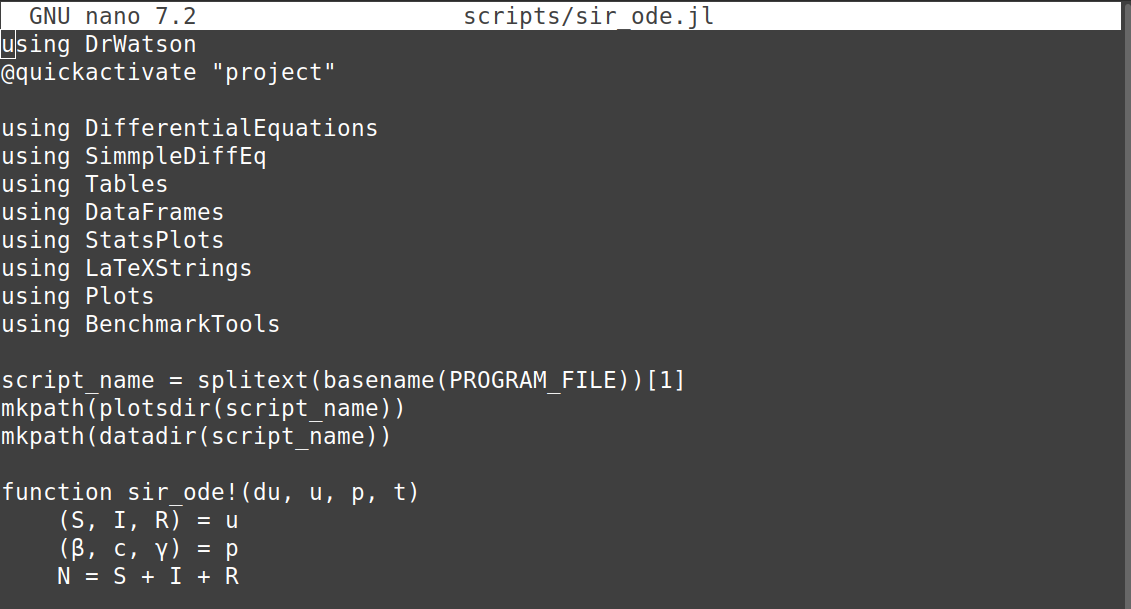
\includegraphics[width=0.7\textwidth,height=\textheight]{image/pic1.png}

}

\caption{\label{fig-001}Код из лабораторного руководства}

\end{figure}%

Я преобразую код в литературный стиль(рис.2)

\begin{figure}

\centering{

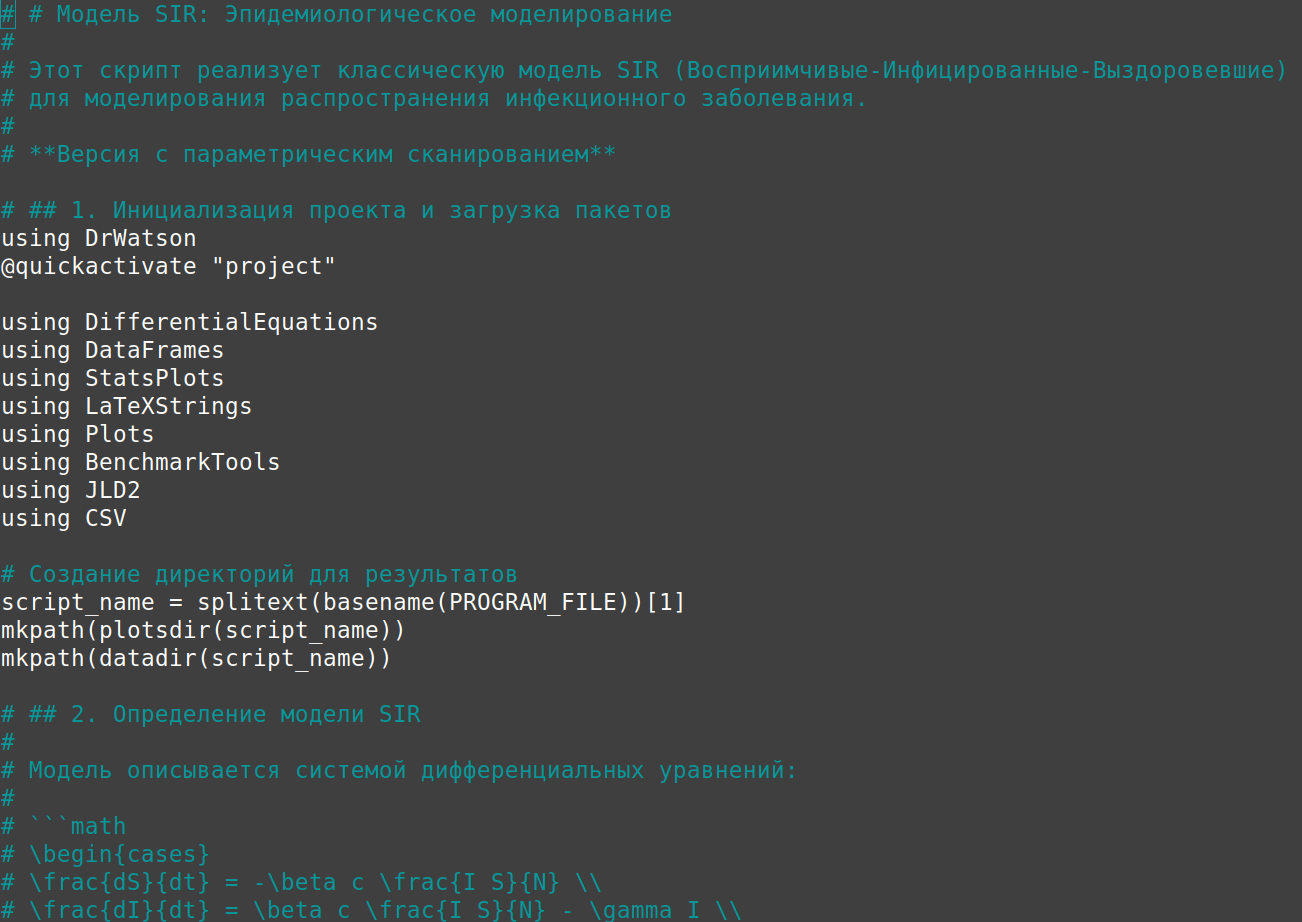
\includegraphics[width=0.7\textwidth,height=\textheight]{image/pic22.png}

}

\caption{\label{fig-002}Код в литературном стиле}

\end{figure}%

После этого я запускаю код, чтобы проверить, работает ли он без ошибок,
и это так(рис.3)

\begin{figure}

\centering{

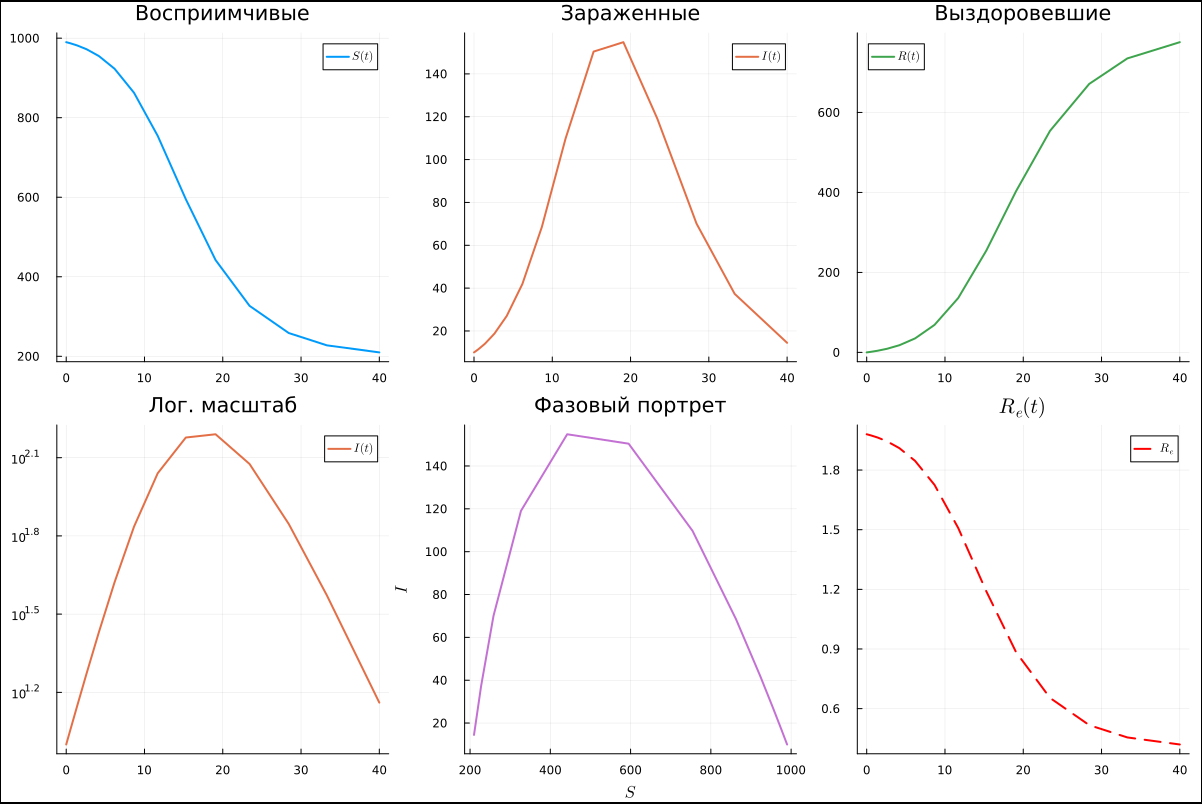
\includegraphics[width=0.7\textwidth,height=\textheight]{image/pic4.png}

}

\caption{\label{fig-003}запуск кода}

\end{figure}%

Затем я создаю файл jupyter notebook, используя файл tangle, который мы
создали ранее. Я запускаю код из файла jupyter notebook, чтобы
убедиться, что он работает без ошибок(рис.4)

\begin{figure}

\centering{

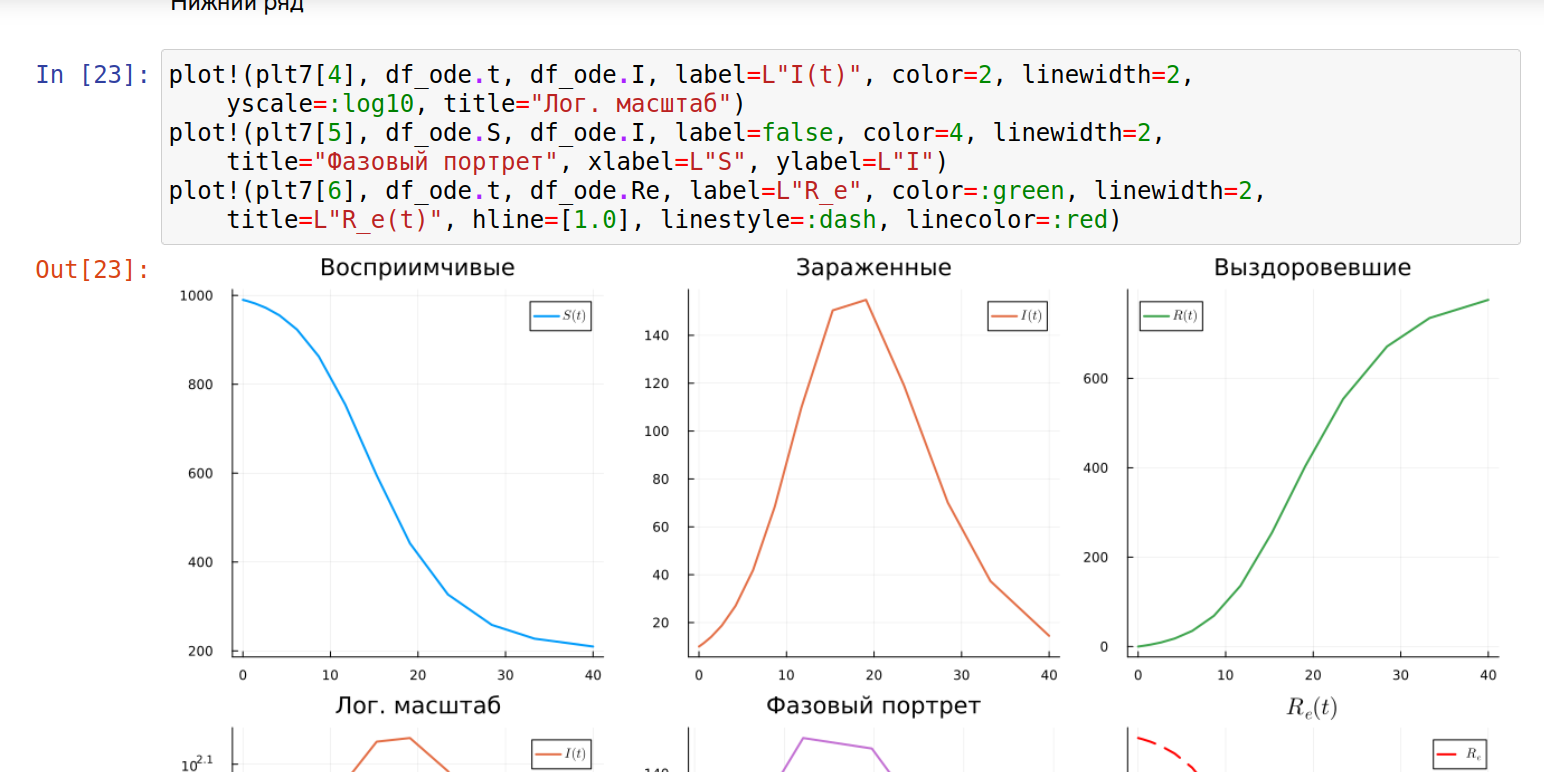
\includegraphics[width=0.7\textwidth,height=\textheight]{image/pic6.png}

}

\caption{\label{fig-004}запуск кода из jupyter notebook}

\end{figure}%

Я добавляю в код расчет для набора параметров в литературном стиле,
чтобы поэкспериментировать с ним.(рис.5)

\begin{figure}

\centering{

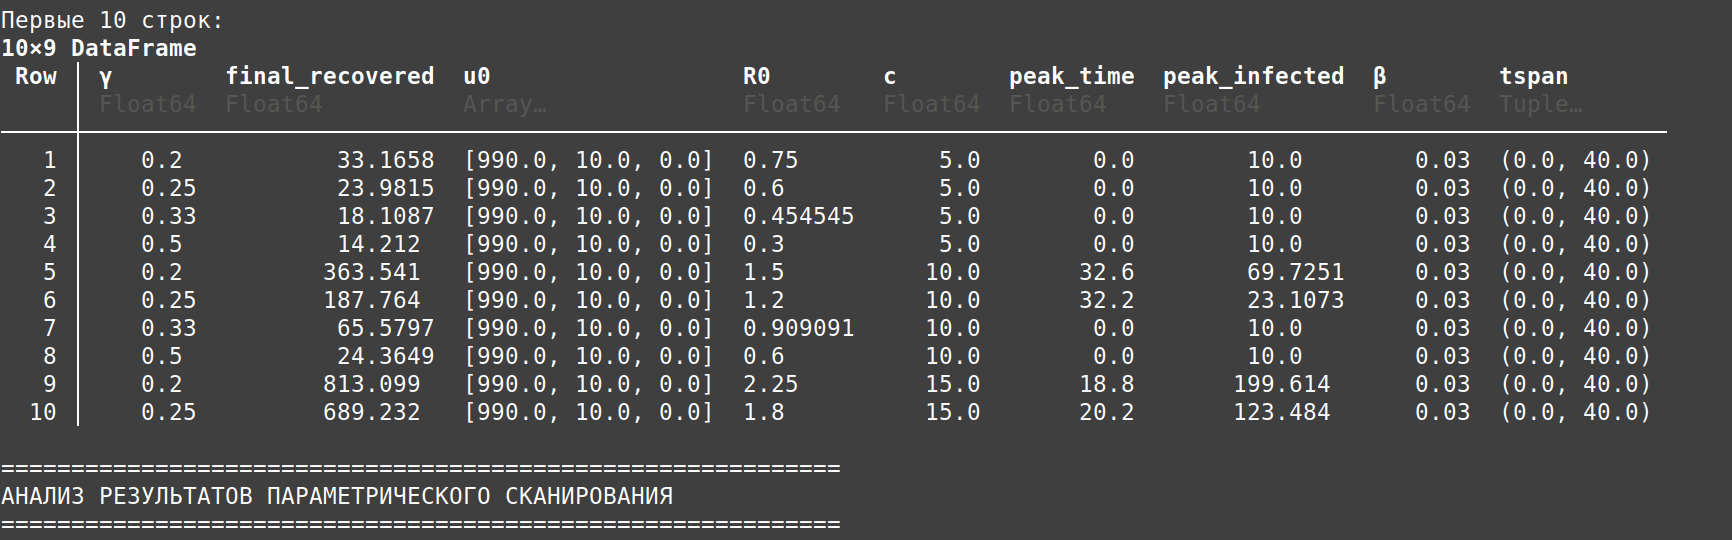
\includegraphics[width=0.7\textwidth,height=\textheight]{image/pic21.png}

}

\caption{\label{fig-005}добавление кода}

\end{figure}%

После этого я запускаю код, чтобы проверить, работает ли он без ошибок,
и это так.В данных видно что при R₀ \textless{} 1 количество зараженных
не растет (остается 10 человек) а при R₀ \textgreater{} 1 начинается
вспышка, чем больше контактов (c), тем сильнее эпидемия и чем быстрее
выздоровление (γ), тем слабее эпидемия.(рис.6)

\begin{figure}

\centering{

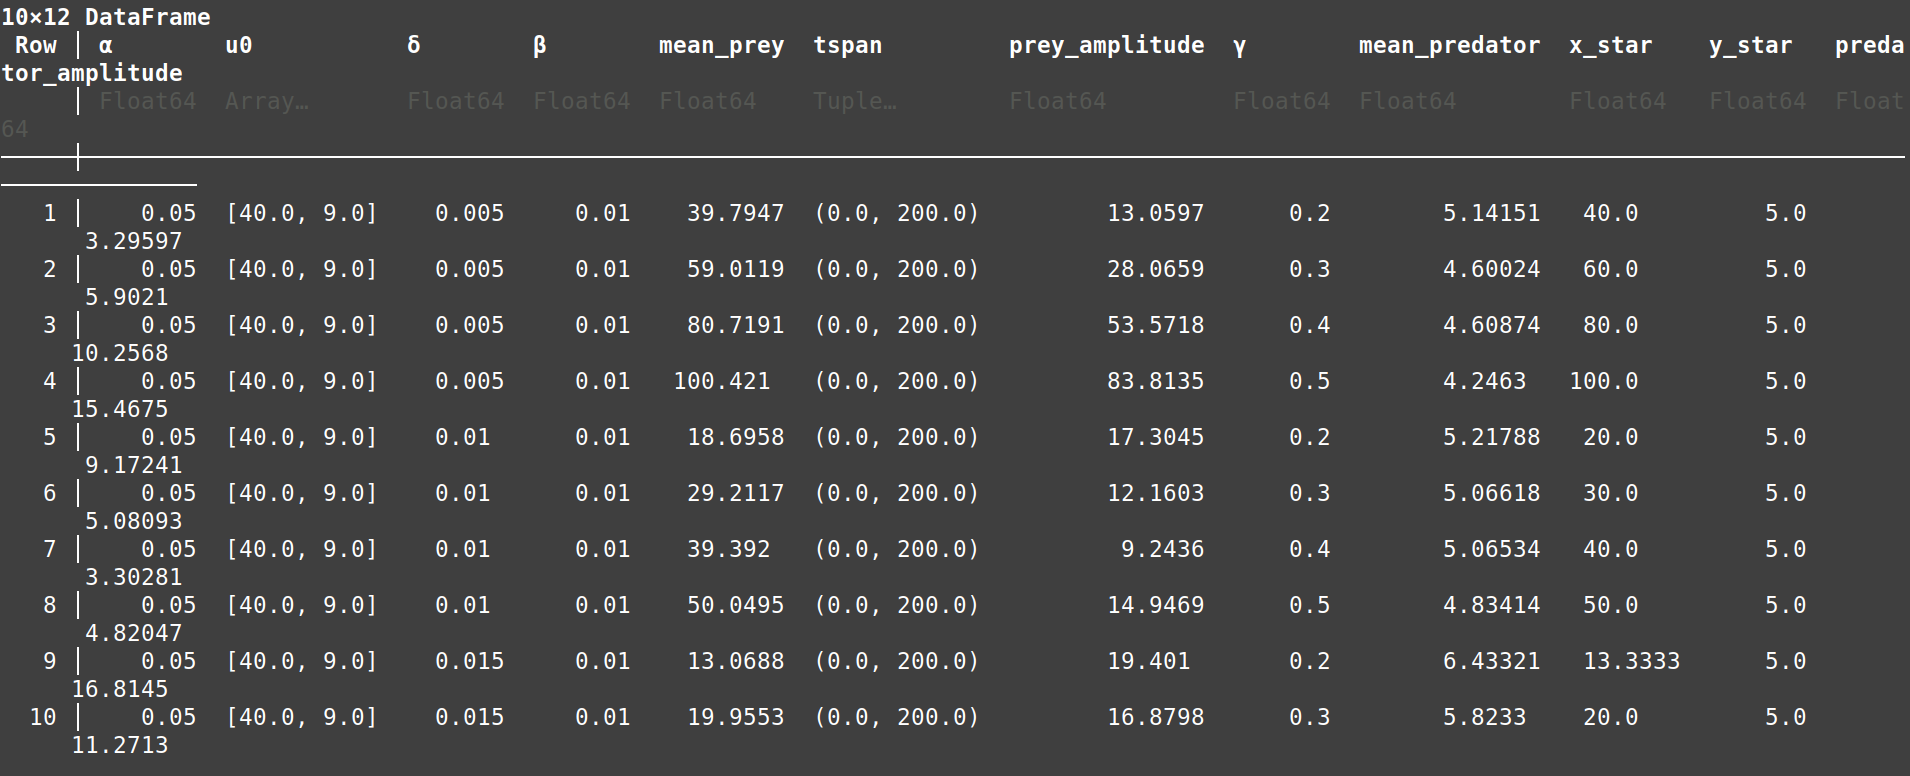
\includegraphics[width=0.7\textwidth,height=\textheight]{image/pic17.png}

}

\caption{\label{fig-006}запуск кода}

\end{figure}%

Затем я создаю файл jupyter notebook, используя файл tangle, который мы
создали ранее. Я запускаю код из файла jupyter notebook, чтобы
убедиться, что он работает без ошибок(рис.7)

\begin{figure}

\centering{

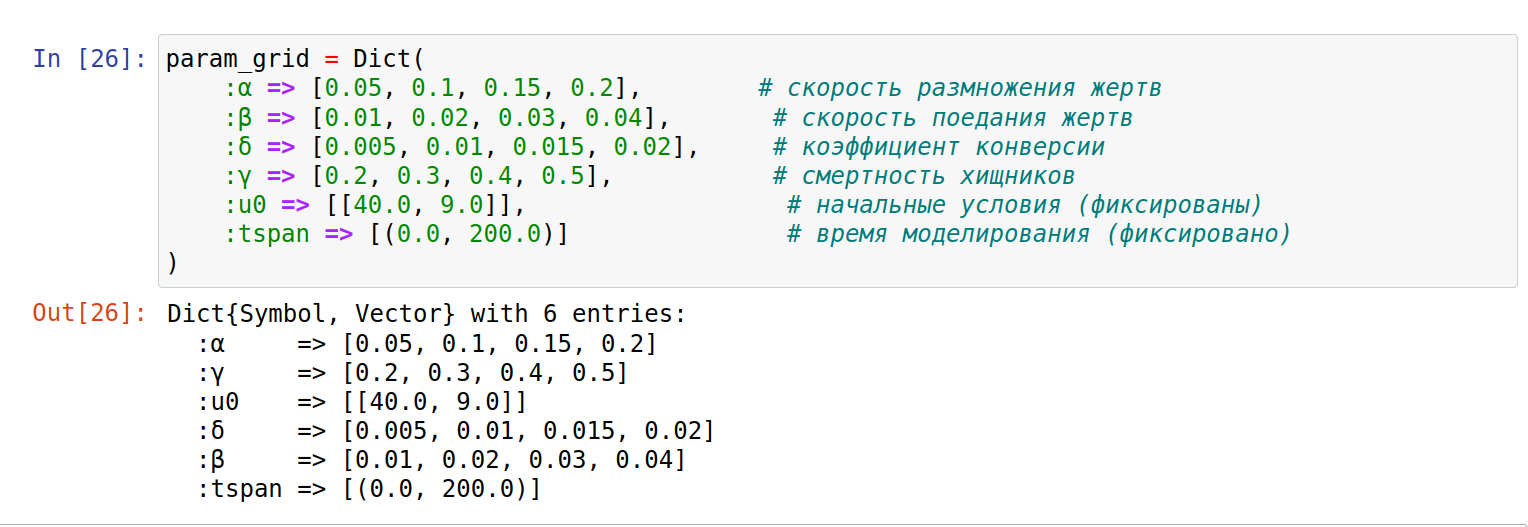
\includegraphics[width=0.7\textwidth,height=\textheight]{image/pic18.png}

}

\caption{\label{fig-007}запуск кода из jupyter notebook}

\end{figure}%

\textbf{\emph{Ниже приведен код, результаты расчетов и графики для кода
в файле sir\_ode1.jl.qmd}}

\chapter{Модель SIR: Эпидемиологическое
моделирование}\label{ux43cux43eux434ux435ux43bux44c-sir-ux44dux43fux438ux434ux435ux43cux438ux43eux43bux43eux433ux438ux447ux435ux441ux43aux43eux435-ux43cux43eux434ux435ux43bux438ux440ux43eux432ux430ux43dux438ux435}

Этот скрипт реализует классическую модель SIR
(Восприимчивые-Инфицированные-Выздоровевшие) для моделирования
распространения инфекционного заболевания.

\textbf{Версия с параметрическим сканированием}

\section{1. Инициализация проекта и загрузка
пакетов}\label{ux438ux43dux438ux446ux438ux430ux43bux438ux437ux430ux446ux438ux44f-ux43fux440ux43eux435ux43aux442ux430-ux438-ux437ux430ux433ux440ux443ux437ux43aux430-ux43fux430ux43aux435ux442ux43eux432}

\begin{Shaded}
\begin{Highlighting}[]
\ImportTok{using} \BuiltInTok{DrWatson}
\PreprocessorTok{@quickactivate} \StringTok{"project"}

\ImportTok{using} \BuiltInTok{DifferentialEquations}
\ImportTok{using} \BuiltInTok{DataFrames}
\ImportTok{using} \BuiltInTok{StatsPlots}
\ImportTok{using} \BuiltInTok{LaTeXStrings}
\ImportTok{using} \BuiltInTok{Plots}
\FunctionTok{gr}\NormalTok{(fmt}\OperatorTok{=:}\NormalTok{png)}
\ImportTok{using} \BuiltInTok{BenchmarkTools}
\ImportTok{using} \BuiltInTok{JLD2}
\ImportTok{using} \BuiltInTok{CSV}
\end{Highlighting}
\end{Shaded}

\begin{verbatim}
┌ Warning: DrWatson could not find find a project file by recursively checking given `dir` and its parents. Returning `nothing` instead.
│ (given dir: /home/nelianjovu)
└ @ DrWatson ~/.julia/packages/DrWatson/2QF5p/src/project_setup.jl:84
\end{verbatim}

Создание директорий для результатов

\begin{Shaded}
\begin{Highlighting}[]
\NormalTok{script\_name }\OperatorTok{=} \FunctionTok{splitext}\NormalTok{(}\FunctionTok{basename}\NormalTok{(}\ConstantTok{PROGRAM\_FILE}\NormalTok{))[}\FloatTok{1}\NormalTok{]}
\FunctionTok{mkpath}\NormalTok{(}\FunctionTok{plotsdir}\NormalTok{(script\_name))}
\FunctionTok{mkpath}\NormalTok{(}\FunctionTok{datadir}\NormalTok{(script\_name))}
\end{Highlighting}
\end{Shaded}

\begin{verbatim}
"/home/nelianjovu/work/study/2026-1/2026-1==study--simulationmod/2026-1--study--simulationmod/labs/lab02/project/data"
\end{verbatim}

\section{2. Определение модели
SIR}\label{ux43eux43fux440ux435ux434ux435ux43bux435ux43dux438ux435-ux43cux43eux434ux435ux43bux438-sir}

Модель описывается системой дифференциальных уравнений:

\begin{Shaded}
\begin{Highlighting}[]
\NormalTok{\textbackslash{}begin\{cases\}}
\NormalTok{\textbackslash{}frac\{dS\}\{dt\} = {-}\textbackslash{}beta c \textbackslash{}frac\{I S\}\{N\} \textbackslash{}\textbackslash{}}
\NormalTok{\textbackslash{}frac\{dI\}\{dt\} = \textbackslash{}beta c \textbackslash{}frac\{I S\}\{N\} {-} \textbackslash{}gamma I \textbackslash{}\textbackslash{}}
\NormalTok{\textbackslash{}frac\{dR\}\{dt\} = \textbackslash{}gamma I}
\NormalTok{\textbackslash{}end\{cases\}}
\end{Highlighting}
\end{Shaded}

где: - \textbf{S} - восприимчивые - \textbf{I} - инфицированные -
\textbf{R} - выздоровевшие - \textbf{β} - вероятность заражения при
контакте - \textbf{c} - среднее число контактов - \textbf{γ} - скорость
выздоровления - \textbf{N = S + I + R} - общая популяция

\begin{Shaded}
\begin{Highlighting}[]
\KeywordTok{function} \FunctionTok{sir\_model!}\NormalTok{(du, u, p, t)}
\NormalTok{    S, I, R }\OperatorTok{=}\NormalTok{ u}
\NormalTok{    β, c, γ }\OperatorTok{=}\NormalTok{ p}
\NormalTok{    N }\OperatorTok{=}\NormalTok{ S }\OperatorTok{+}\NormalTok{ I }\OperatorTok{+}\NormalTok{ R}
    \PreprocessorTok{@inbounds} \ControlFlowTok{begin}
\NormalTok{        du[}\FloatTok{1}\NormalTok{] }\OperatorTok{=} \OperatorTok{{-}}\NormalTok{β }\OperatorTok{*}\NormalTok{ c }\OperatorTok{*}\NormalTok{ I }\OperatorTok{*}\NormalTok{ S }\OperatorTok{/}\NormalTok{ N}
\NormalTok{        du[}\FloatTok{2}\NormalTok{] }\OperatorTok{=}\NormalTok{ β }\OperatorTok{*}\NormalTok{ c }\OperatorTok{*}\NormalTok{ I }\OperatorTok{*}\NormalTok{ S }\OperatorTok{/}\NormalTok{ N }\OperatorTok{{-}}\NormalTok{ γ }\OperatorTok{*}\NormalTok{ I}
\NormalTok{        du[}\FloatTok{3}\NormalTok{] }\OperatorTok{=}\NormalTok{ γ }\OperatorTok{*}\NormalTok{ I}
    \ControlFlowTok{end}
    \ConstantTok{nothing}
\KeywordTok{end}
\end{Highlighting}
\end{Shaded}

\begin{verbatim}
sir_model! (generic function with 1 method)
\end{verbatim}

\section{3. Базовые параметры
модели}\label{ux431ux430ux437ux43eux432ux44bux435-ux43fux430ux440ux430ux43cux435ux442ux440ux44b-ux43cux43eux434ux435ux43bux438}

Для типичной респираторной инфекции: - \textbf{β = 0.05} (5\%
вероятность заражения при контакте) - \textbf{c = 10} (10 контактов в
день) - \textbf{γ = 0.25} (выздоровление за 4 дня в среднем) -
\textbf{Начальные условия}: S₀ = 990, I₀ = 10, R₀ = 0 - \textbf{Время
моделирования}: 40 дней

\begin{Shaded}
\begin{Highlighting}[]
\NormalTok{δt }\OperatorTok{=} \FloatTok{0.1}
\NormalTok{tmax }\OperatorTok{=} \FloatTok{40.0}
\NormalTok{tspan }\OperatorTok{=}\NormalTok{ (}\FloatTok{0.0}\NormalTok{, tmax)}
\NormalTok{u0 }\OperatorTok{=}\NormalTok{ [}\FloatTok{990.0}\NormalTok{, }\FloatTok{10.0}\NormalTok{, }\FloatTok{0.0}\NormalTok{]}
\NormalTok{base\_params }\OperatorTok{=}\NormalTok{ [}\FloatTok{0.05}\NormalTok{, }\FloatTok{10.0}\NormalTok{, }\FloatTok{0.25}\NormalTok{]}
\end{Highlighting}
\end{Shaded}

\begin{verbatim}
3-element Vector{Float64}:
  0.05
 10.0
  0.25
\end{verbatim}

\subsection{Базовое репродуктивное
число}\label{ux431ux430ux437ux43eux432ux43eux435-ux440ux435ux43fux440ux43eux434ux443ux43aux442ux438ux432ux43dux43eux435-ux447ux438ux441ux43bux43e}

\begin{Shaded}
\begin{Highlighting}[]
\NormalTok{R\_0 = \textbackslash{}frac\{c \textbackslash{}cdot \textbackslash{}beta\}\{\textbackslash{}gamma\}}
\end{Highlighting}
\end{Shaded}

При R₀ \textgreater{} 1 эпидемия растёт, при R₀ \textless{} 1 -
затухает.

\begin{Shaded}
\begin{Highlighting}[]
\NormalTok{R0\_base }\OperatorTok{=}\NormalTok{ (base\_params[}\FloatTok{2}\NormalTok{] }\OperatorTok{*}\NormalTok{ base\_params[}\FloatTok{1}\NormalTok{]) }\OperatorTok{/}\NormalTok{ base\_params[}\FloatTok{3}\NormalTok{]}

\FunctionTok{println}\NormalTok{(}\StringTok{"="}\OperatorTok{\^{}}\FloatTok{60}\NormalTok{)}
\FunctionTok{println}\NormalTok{(}\StringTok{"МОДЕЛЬ SIR: Базовые параметры"}\NormalTok{)}
\FunctionTok{println}\NormalTok{(}\StringTok{"="}\OperatorTok{\^{}}\FloatTok{60}\NormalTok{)}
\FunctionTok{println}\NormalTok{(}\StringTok{"β (вероятность заражения) = "}\NormalTok{, base\_params[}\FloatTok{1}\NormalTok{])}
\FunctionTok{println}\NormalTok{(}\StringTok{"c (среднее число контактов) = "}\NormalTok{, base\_params[}\FloatTok{2}\NormalTok{])}
\FunctionTok{println}\NormalTok{(}\StringTok{"γ (скорость выздоровления) = "}\NormalTok{, base\_params[}\FloatTok{3}\NormalTok{])}
\FunctionTok{println}\NormalTok{(}\StringTok{"R₀ = c·β/γ = "}\NormalTok{, }\FunctionTok{round}\NormalTok{(R0\_base, digits}\OperatorTok{=}\FloatTok{3}\NormalTok{))}
\FunctionTok{println}\NormalTok{(}\StringTok{"Средняя продолжительность болезни = "}\NormalTok{, }\FunctionTok{round}\NormalTok{(}\FloatTok{1}\OperatorTok{/}\NormalTok{base\_params[}\FloatTok{3}\NormalTok{], digits}\OperatorTok{=}\FloatTok{2}\NormalTok{), }\StringTok{" дней"}\NormalTok{)}
\FunctionTok{println}\NormalTok{(}\StringTok{"Начальные условия: S₀ = "}\NormalTok{, u0[}\FloatTok{1}\NormalTok{], }\StringTok{", I₀ = "}\NormalTok{, u0[}\FloatTok{2}\NormalTok{], }\StringTok{", R₀ = "}\NormalTok{, u0[}\FloatTok{3}\NormalTok{])}
\end{Highlighting}
\end{Shaded}

\begin{verbatim}
============================================================
МОДЕЛЬ SIR: Базовые параметры
============================================================
β (вероятность заражения) = 0.05
c (среднее число контактов) = 10.0
γ (скорость выздоровления) = 0.25
R₀ = c·β/γ = 2.0
Средняя продолжительность болезни = 4.0 дней
Начальные условия: S₀ = 990.0, I₀ = 10.0, R₀ = 0.0
\end{verbatim}

\section{4. Численное решение (базовый
эксперимент)}\label{ux447ux438ux441ux43bux435ux43dux43dux43eux435-ux440ux435ux448ux435ux43dux438ux435-ux431ux430ux437ux43eux432ux44bux439-ux44dux43aux441ux43fux435ux440ux438ux43cux435ux43dux442}

\begin{Shaded}
\begin{Highlighting}[]
\NormalTok{prob\_base }\OperatorTok{=} \FunctionTok{ODEProblem}\NormalTok{(sir\_model!, u0, tspan, base\_params)}
\NormalTok{sol\_base }\OperatorTok{=} \FunctionTok{solve}\NormalTok{(prob\_base, dt }\OperatorTok{=}\NormalTok{ δt)}
\end{Highlighting}
\end{Shaded}

\begin{verbatim}
retcode: Success
Interpolation: 3rd order Hermite
t: 15-element Vector{Float64}:
  0.0
  0.1
  0.5331242537191838
  1.3919008491040001
  2.6102120755226386
  4.1811820758323055
  6.180123810566044
  8.664951930903612
 11.691425331813486
 15.279370667110317
 19.082963490744028
 23.423425193442526
 28.42949373098617
 33.298779173639595
 40.0
u: 15-element Vector{Vector{Float64}}:
 [990.0, 10.0, 0.0]
 [989.4990153200853, 10.247898072276145, 0.25308660763853114]
 [987.1852964117763, 11.391111426852985, 1.4235921613706282]
 [981.8312125227972, 14.026022042698546, 4.142765434504279]
 [972.1392310589528, 18.757815561654184, 9.102953379393007]
 [954.9905500491583, 27.007702518267585, 18.001747432574028]
 [923.0706717929863, 41.9297677983272, 34.9995604086864]
 [862.6705810342164, 68.49345419063418, 68.8359647751493]
 [754.3022993851442, 109.74186185409286, 135.95583876076284]
 [595.1014268847732, 150.41363264480714, 254.4849404704195]
 [442.01411791012964, 154.80694988491865, 403.17893220495154]
 [326.8951167493957, 119.06860394684863, 554.0362793037555]
 [258.50852421889647, 70.11052194753061, 671.3809538335727]
 [227.5833833708572, 37.32857063157993, 735.0880459975626]
 [209.84121402014358, 14.473644966455783, 775.6851410134004]
\end{verbatim}

Подготовка данных для анализа

\begin{Shaded}
\begin{Highlighting}[]
\NormalTok{df\_base }\OperatorTok{=} \FunctionTok{DataFrame}\NormalTok{(Tables.}\FunctionTok{table}\NormalTok{(sol\_base}\OperatorTok{\textquotesingle{}}\NormalTok{))}
\FunctionTok{rename!}\NormalTok{(df\_base, [}\StringTok{"S"}\NormalTok{, }\StringTok{"I"}\NormalTok{, }\StringTok{"R"}\NormalTok{])}
\NormalTok{df\_base[!, }\OperatorTok{:}\NormalTok{t] }\OperatorTok{=}\NormalTok{ sol\_base.t}
\NormalTok{df\_base[!, }\OperatorTok{:}\NormalTok{N] }\OperatorTok{=}\NormalTok{ df\_base.S }\OperatorTok{+}\NormalTok{ df\_base.I }\OperatorTok{+}\NormalTok{ df\_base.R}
\end{Highlighting}
\end{Shaded}

\begin{verbatim}
15-element Vector{Float64}:
 1000.0
 1000.0
  999.9999999999999
 1000.0
 1000.0
  999.9999999999999
 1000.0
  999.9999999999999
 1000.0
  999.9999999999999
  999.9999999999998
  999.9999999999998
  999.9999999999998
  999.9999999999998
  999.9999999999998
\end{verbatim}

\section{5. Визуализация базового
эксперимента}\label{ux432ux438ux437ux443ux430ux43bux438ux437ux430ux446ux438ux44f-ux431ux430ux437ux43eux432ux43eux433ux43e-ux44dux43aux441ux43fux435ux440ux438ux43cux435ux43dux442ux430}

\subsection{5.1 Динамика всех групп
населения}\label{ux434ux438ux43dux430ux43cux438ux43aux430-ux432ux441ux435ux445-ux433ux440ux443ux43fux43f-ux43dux430ux441ux435ux43bux435ux43dux438ux44f}

\begin{Shaded}
\begin{Highlighting}[]
\NormalTok{plt1 }\OperatorTok{=} \FunctionTok{plot}\NormalTok{(df\_base.t, [df\_base.S df\_base.I df\_base.R],}
\NormalTok{    label}\OperatorTok{=}\NormalTok{[L}\StringTok{"S(t)"}\NormalTok{ L}\StringTok{"I(t)"}\NormalTok{ L}\StringTok{"R(t)"}\NormalTok{],}
\NormalTok{    xlabel}\OperatorTok{=}\StringTok{"Время, дни"}\NormalTok{,}
\NormalTok{    ylabel}\OperatorTok{=}\StringTok{"Количество людей"}\NormalTok{,}
\NormalTok{    title}\OperatorTok{=}\StringTok{"Модель SIR: Базовая динамика"}\NormalTok{,}
\NormalTok{    linewidth}\OperatorTok{=}\FloatTok{2}\NormalTok{,}
\NormalTok{    legend}\OperatorTok{=:}\NormalTok{right,}
\NormalTok{    grid}\OperatorTok{=}\ConstantTok{true}\NormalTok{,}
\NormalTok{    size}\OperatorTok{=}\NormalTok{(}\FloatTok{800}\NormalTok{, }\FloatTok{500}\NormalTok{))}

\FunctionTok{annotate!}\NormalTok{(plt1,}
    \FunctionTok{maximum}\NormalTok{(df\_base.t) }\OperatorTok{*} \FloatTok{0.7}\NormalTok{,}
    \FunctionTok{maximum}\NormalTok{(df\_base.N) }\OperatorTok{*} \FloatTok{0.8}\NormalTok{,}
    \FunctionTok{text}\NormalTok{(}\StringTok{"Базовые параметры:}\SpecialCharTok{\textbackslash{}n}\StringTok{β = }\SpecialCharTok{$}\NormalTok{(base\_params[}\FloatTok{1}\NormalTok{])}\SpecialCharTok{\textbackslash{}n}\StringTok{c = }\SpecialCharTok{$}\NormalTok{(base\_params[}\FloatTok{2}\NormalTok{])}\SpecialCharTok{\textbackslash{}n}\StringTok{γ = }\SpecialCharTok{$}\NormalTok{(base\_params[}\FloatTok{3}\NormalTok{])}\SpecialCharTok{\textbackslash{}n}\StringTok{R₀ = }\SpecialCharTok{$}\NormalTok{(}\FunctionTok{round}\NormalTok{(R0\_base, digits}\OperatorTok{=}\FloatTok{2}\NormalTok{))}\StringTok{"}\NormalTok{,}
    \FloatTok{8}\NormalTok{, }\OperatorTok{:}\NormalTok{left))}
\end{Highlighting}
\end{Shaded}

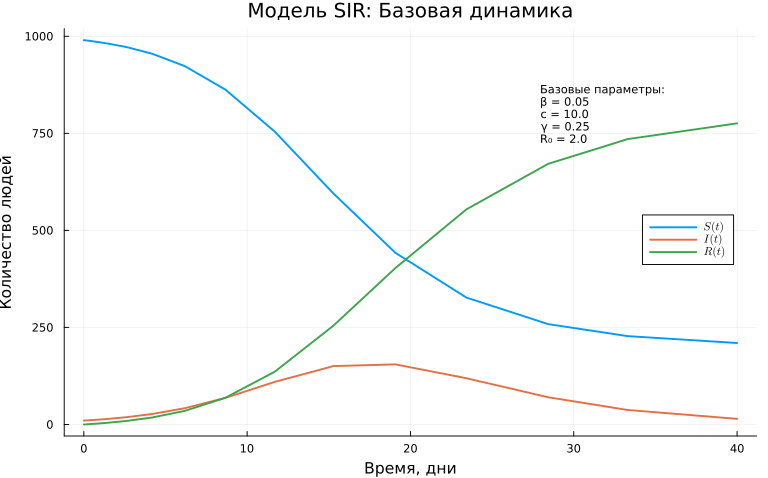
\includegraphics{simmod-lab02-report (Нелиа Нджову)_files/figure-pdf/cell-10-output-1.png}

Поиск пика для базового эксперимента

\begin{Shaded}
\begin{Highlighting}[]
\NormalTok{peak\_idx }\OperatorTok{=} \FunctionTok{argmax}\NormalTok{(df\_base.I)}
\NormalTok{peak\_time\_base }\OperatorTok{=}\NormalTok{ df\_base.t[peak\_idx]}
\NormalTok{peak\_value\_base }\OperatorTok{=}\NormalTok{ df\_base.I[peak\_idx]}
\end{Highlighting}
\end{Shaded}

\begin{verbatim}
154.80694988491865
\end{verbatim}

\subsection{5.2 Динамика инфицированных (с выделением
пика)}\label{ux434ux438ux43dux430ux43cux438ux43aux430-ux438ux43dux444ux438ux446ux438ux440ux43eux432ux430ux43dux43dux44bux445-ux441-ux432ux44bux434ux435ux43bux435ux43dux438ux435ux43c-ux43fux438ux43aux430}

\begin{Shaded}
\begin{Highlighting}[]
\NormalTok{plt2 }\OperatorTok{=} \FunctionTok{plot}\NormalTok{(df\_base.t, df\_base.I,}
\NormalTok{    label}\OperatorTok{=}\NormalTok{L}\StringTok{"I(t)"}\NormalTok{,}
\NormalTok{    xlabel}\OperatorTok{=}\StringTok{"Время, дни"}\NormalTok{,}
\NormalTok{    ylabel}\OperatorTok{=}\StringTok{"Количество инфицированных"}\NormalTok{,}
\NormalTok{    title}\OperatorTok{=}\StringTok{"Динамика числа зараженных"}\NormalTok{,}
\NormalTok{    color}\OperatorTok{=:}\NormalTok{red,}
\NormalTok{    linewidth}\OperatorTok{=}\FloatTok{2}\NormalTok{,}
\NormalTok{    fill}\OperatorTok{=}\NormalTok{(}\FloatTok{0}\NormalTok{, }\FloatTok{0.3}\NormalTok{, }\OperatorTok{:}\NormalTok{red),}
\NormalTok{    grid}\OperatorTok{=}\ConstantTok{true}\NormalTok{,}
\NormalTok{    size}\OperatorTok{=}\NormalTok{(}\FloatTok{800}\NormalTok{, }\FloatTok{400}\NormalTok{))}

\FunctionTok{vline!}\NormalTok{(plt2, [peak\_time\_base], color}\OperatorTok{=:}\NormalTok{black, linestyle}\OperatorTok{=:}\NormalTok{dash, label}\OperatorTok{=}\ConstantTok{false}\NormalTok{)}
\FunctionTok{annotate!}\NormalTok{(plt2, peak\_time\_base, peak\_value\_base }\OperatorTok{*} \FloatTok{1.05}\NormalTok{,}
    \FunctionTok{text}\NormalTok{(}\StringTok{"Пик: }\SpecialCharTok{$}\NormalTok{(}\FunctionTok{round}\NormalTok{(peak\_value\_base, digits}\OperatorTok{=}\FloatTok{1}\NormalTok{))}\SpecialCharTok{\textbackslash{}n}\StringTok{на }\SpecialCharTok{$}\NormalTok{(}\FunctionTok{round}\NormalTok{(peak\_time\_base, digits}\OperatorTok{=}\FloatTok{1}\NormalTok{))}\StringTok{ день"}\NormalTok{, }\FloatTok{8}\NormalTok{, }\OperatorTok{:}\NormalTok{top))}
\end{Highlighting}
\end{Shaded}

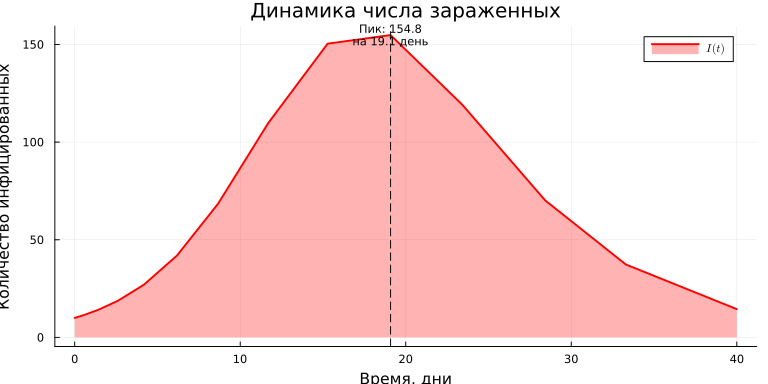
\includegraphics{simmod-lab02-report (Нелиа Нджову)_files/figure-pdf/cell-12-output-1.png}

\subsection{5.3 Логарифмический
масштаб}\label{ux43bux43eux433ux430ux440ux438ux444ux43cux438ux447ux435ux441ux43aux438ux439-ux43cux430ux441ux448ux442ux430ux431}

\begin{Shaded}
\begin{Highlighting}[]
\NormalTok{plt3 }\OperatorTok{=} \FunctionTok{plot}\NormalTok{(df\_base.t, df\_base.I,}
\NormalTok{    label}\OperatorTok{=}\NormalTok{L}\StringTok{"I(t)"}\NormalTok{,}
\NormalTok{    xlabel}\OperatorTok{=}\StringTok{"Время, дни"}\NormalTok{,}
\NormalTok{    ylabel}\OperatorTok{=}\StringTok{"log(Инфицированные)"}\NormalTok{,}
\NormalTok{    title}\OperatorTok{=}\StringTok{"Экспоненциальный рост (лог. шкала)"}\NormalTok{,}
\NormalTok{    yscale}\OperatorTok{=:}\NormalTok{log10,}
\NormalTok{    color}\OperatorTok{=:}\NormalTok{red,}
\NormalTok{    linewidth}\OperatorTok{=}\FloatTok{2}\NormalTok{,}
\NormalTok{    grid}\OperatorTok{=}\ConstantTok{true}\NormalTok{,}
\NormalTok{    size}\OperatorTok{=}\NormalTok{(}\FloatTok{800}\NormalTok{, }\FloatTok{400}\NormalTok{))}
\end{Highlighting}
\end{Shaded}

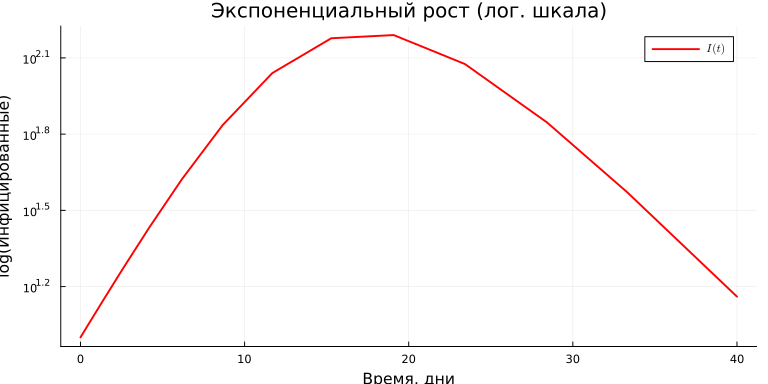
\includegraphics{simmod-lab02-report (Нелиа Нджову)_files/figure-pdf/cell-13-output-1.png}

\subsection{5.4 Доли населения в
процентах}\label{ux434ux43eux43bux438-ux43dux430ux441ux435ux43bux435ux43dux438ux44f-ux432-ux43fux440ux43eux446ux435ux43dux442ux430ux445}

\begin{Shaded}
\begin{Highlighting}[]
\NormalTok{plt4 }\OperatorTok{=} \FunctionTok{plot}\NormalTok{(df\_base.t,}
\NormalTok{    [df\_base.S df\_base.I df\_base.R] }\OperatorTok{./}\NormalTok{ df\_base.N }\OperatorTok{.*} \FloatTok{100}\NormalTok{,}
\NormalTok{    label}\OperatorTok{=}\NormalTok{[L}\StringTok{"S(t)/N"}\NormalTok{ L}\StringTok{"I(t)/N"}\NormalTok{ L}\StringTok{"R(t)/N"}\NormalTok{],}
\NormalTok{    xlabel}\OperatorTok{=}\StringTok{"Время, дни"}\NormalTok{,}
\NormalTok{    ylabel}\OperatorTok{=}\StringTok{"Доля популяции, \%"}\NormalTok{,}
\NormalTok{    title}\OperatorTok{=}\StringTok{"Динамика эпидемии (в процентах)"}\NormalTok{,}
\NormalTok{    linewidth}\OperatorTok{=}\FloatTok{2}\NormalTok{,}
\NormalTok{    legend}\OperatorTok{=:}\NormalTok{right,}
\NormalTok{    grid}\OperatorTok{=}\ConstantTok{true}\NormalTok{,}
\NormalTok{    size}\OperatorTok{=}\NormalTok{(}\FloatTok{800}\NormalTok{, }\FloatTok{500}\NormalTok{))}

\ControlFlowTok{if}\NormalTok{ R0\_base }\OperatorTok{\textgreater{}} \FloatTok{1}
\NormalTok{    herd\_immunity }\OperatorTok{=}\NormalTok{ (}\FloatTok{1} \OperatorTok{{-}} \FloatTok{1}\OperatorTok{/}\NormalTok{R0\_base) }\OperatorTok{*} \FloatTok{100}
    \FunctionTok{hline!}\NormalTok{(plt4, [herd\_immunity],}
\NormalTok{        color}\OperatorTok{=:}\NormalTok{purple,}
\NormalTok{        linestyle}\OperatorTok{=:}\NormalTok{dash,}
\NormalTok{        label}\OperatorTok{=}\StringTok{"Коллективный иммунитет (}\SpecialCharTok{$}\NormalTok{(}\FunctionTok{round}\NormalTok{(herd\_immunity, digits}\OperatorTok{=}\FloatTok{1}\NormalTok{))}\StringTok{\%)"}\NormalTok{,}
\NormalTok{        linewidth}\OperatorTok{=}\FloatTok{1.5}\NormalTok{)}
\ControlFlowTok{end}
\end{Highlighting}
\end{Shaded}

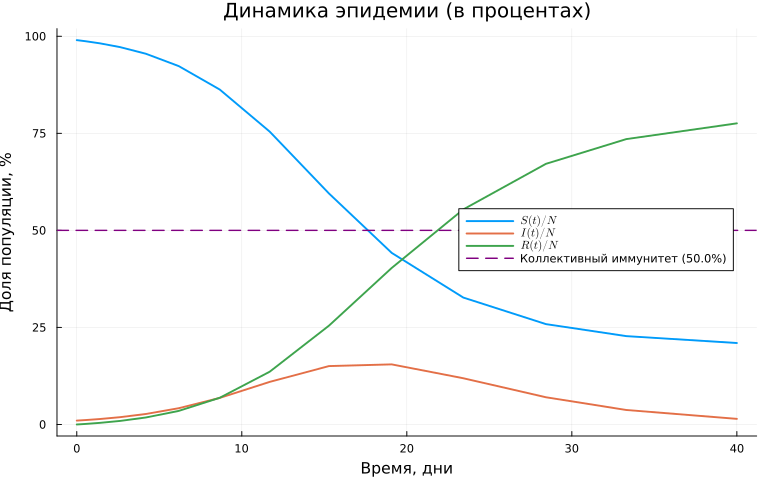
\includegraphics{simmod-lab02-report (Нелиа Нджову)_files/figure-pdf/cell-14-output-1.png}

\subsection{5.5 Фазовый
портрет}\label{ux444ux430ux437ux43eux432ux44bux439-ux43fux43eux440ux442ux440ux435ux442}

\begin{Shaded}
\begin{Highlighting}[]
\NormalTok{plt5 }\OperatorTok{=} \FunctionTok{plot}\NormalTok{(df\_base.S, df\_base.I,}
\NormalTok{    label}\OperatorTok{=}\StringTok{"Фазовая траектория"}\NormalTok{,}
\NormalTok{    xlabel}\OperatorTok{=}\NormalTok{L}\StringTok{"S(t)"}\NormalTok{,}
\NormalTok{    ylabel}\OperatorTok{=}\NormalTok{L}\StringTok{"I(t)"}\NormalTok{,}
\NormalTok{    title}\OperatorTok{=}\StringTok{"Фазовый портрет SIR модели"}\NormalTok{,}
\NormalTok{    color}\OperatorTok{=:}\NormalTok{blue,}
\NormalTok{    linewidth}\OperatorTok{=}\FloatTok{2}\NormalTok{,}
\NormalTok{    grid}\OperatorTok{=}\ConstantTok{true}\NormalTok{,}
\NormalTok{    size}\OperatorTok{=}\NormalTok{(}\FloatTok{800}\NormalTok{, }\FloatTok{500}\NormalTok{))}

\ControlFlowTok{for}\NormalTok{ i }\KeywordTok{in} \FloatTok{1}\OperatorTok{:}\FloatTok{50}\OperatorTok{:}\FunctionTok{length}\NormalTok{(df\_base.S)}\OperatorTok{{-}}\FloatTok{1}
    \FunctionTok{plot!}\NormalTok{(plt5,}
\NormalTok{        [df\_base.S[i], df\_base.S[i}\OperatorTok{+}\FloatTok{1}\NormalTok{]],}
\NormalTok{        [df\_base.I[i], df\_base.I[i}\OperatorTok{+}\FloatTok{1}\NormalTok{]],}
\NormalTok{        arrow}\OperatorTok{=:}\NormalTok{closed, color}\OperatorTok{=:}\NormalTok{blue, alpha}\OperatorTok{=}\FloatTok{0.5}\NormalTok{, label}\OperatorTok{=}\ConstantTok{false}\NormalTok{)}
\ControlFlowTok{end}
\end{Highlighting}
\end{Shaded}

\subsection{5.6 Эффективное репродуктивное
число}\label{ux44dux444ux444ux435ux43aux442ux438ux432ux43dux43eux435-ux440ux435ux43fux440ux43eux434ux443ux43aux442ux438ux432ux43dux43eux435-ux447ux438ux441ux43bux43e}

\begin{Shaded}
\begin{Highlighting}[]
\NormalTok{df\_base[!, }\OperatorTok{:}\NormalTok{Re] }\OperatorTok{=}\NormalTok{ R0\_base }\OperatorTok{.*}\NormalTok{ df\_base.S }\OperatorTok{./}\NormalTok{ df\_base.N}

\NormalTok{plt6 }\OperatorTok{=} \FunctionTok{plot}\NormalTok{(df\_base.t, df\_base.Re,}
\NormalTok{    label}\OperatorTok{=}\NormalTok{L}\StringTok{"R\_e(t)"}\NormalTok{,}
\NormalTok{    xlabel}\OperatorTok{=}\StringTok{"Время, дни"}\NormalTok{,}
\NormalTok{    ylabel}\OperatorTok{=}\NormalTok{L}\StringTok{"R\_e"}\NormalTok{,}
\NormalTok{    title}\OperatorTok{=}\StringTok{"Эффективное репродуктивное число"}\NormalTok{,}
\NormalTok{    color}\OperatorTok{=:}\NormalTok{green,}
\NormalTok{    linewidth}\OperatorTok{=}\FloatTok{2}\NormalTok{,}
\NormalTok{    grid}\OperatorTok{=}\ConstantTok{true}\NormalTok{,}
\NormalTok{    size}\OperatorTok{=}\NormalTok{(}\FloatTok{800}\NormalTok{, }\FloatTok{400}\NormalTok{))}

\FunctionTok{hline!}\NormalTok{(plt6, [}\FloatTok{1.0}\NormalTok{], color}\OperatorTok{=:}\NormalTok{red, linestyle}\OperatorTok{=:}\NormalTok{dash, label}\OperatorTok{=}\StringTok{"Rₑ = 1"}\NormalTok{, linewidth}\OperatorTok{=}\FloatTok{1.5}\NormalTok{)}
\end{Highlighting}
\end{Shaded}

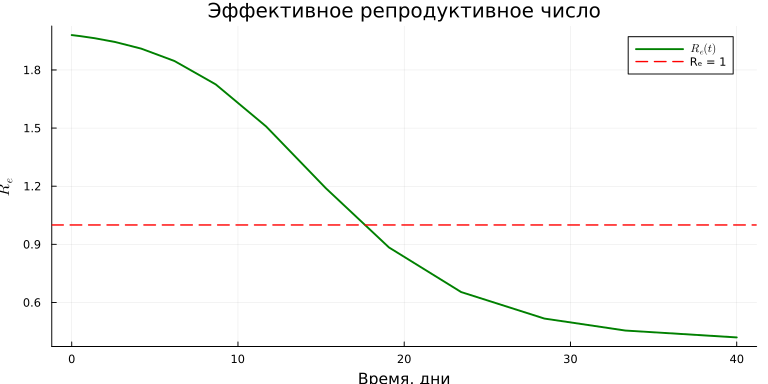
\includegraphics{simmod-lab02-report (Нелиа Нджову)_files/figure-pdf/cell-16-output-1.png}

\section{6. Анализ базового
эксперимента}\label{ux430ux43dux430ux43bux438ux437-ux431ux430ux437ux43eux432ux43eux433ux43e-ux44dux43aux441ux43fux435ux440ux438ux43cux435ux43dux442ux430}

\begin{Shaded}
\begin{Highlighting}[]
\FunctionTok{println}\NormalTok{(}\StringTok{"}\SpecialCharTok{\textbackslash{}n}\StringTok{"} \OperatorTok{*} \StringTok{"="}\OperatorTok{\^{}}\FloatTok{60}\NormalTok{)}
\FunctionTok{println}\NormalTok{(}\StringTok{"РЕЗУЛЬТАТЫ БАЗОВОГО ЭКСПЕРИМЕНТА"}\NormalTok{)}
\FunctionTok{println}\NormalTok{(}\StringTok{"="}\OperatorTok{\^{}}\FloatTok{60}\NormalTok{)}
\FunctionTok{println}\NormalTok{(}\StringTok{"Пик эпидемии: I\_max = }\SpecialCharTok{$}\NormalTok{(}\FunctionTok{round}\NormalTok{(peak\_value\_base, digits}\OperatorTok{=}\FloatTok{1}\NormalTok{))}\StringTok{ на }\SpecialCharTok{$}\NormalTok{(}\FunctionTok{round}\NormalTok{(peak\_time\_base, digits}\OperatorTok{=}\FloatTok{1}\NormalTok{))}\StringTok{ день"}\NormalTok{)}
\FunctionTok{println}\NormalTok{(}\StringTok{"Итоговое число переболевших: R(∞) = }\SpecialCharTok{$}\NormalTok{(}\FunctionTok{round}\NormalTok{(df\_base.R[}\KeywordTok{end}\NormalTok{], digits}\OperatorTok{=}\FloatTok{1}\NormalTok{))}\StringTok{"}\NormalTok{)}
\FunctionTok{println}\NormalTok{(}\StringTok{"Доля переболевших: }\SpecialCharTok{$}\NormalTok{(}\FunctionTok{round}\NormalTok{(df\_base.R[}\KeywordTok{end}\NormalTok{]}\OperatorTok{/}\NormalTok{df\_base.N[}\FloatTok{1}\NormalTok{]}\OperatorTok{*}\FloatTok{100}\NormalTok{, digits}\OperatorTok{=}\FloatTok{1}\NormalTok{))}\StringTok{\%"}\NormalTok{)}
\end{Highlighting}
\end{Shaded}

\begin{verbatim}

============================================================
РЕЗУЛЬТАТЫ БАЗОВОГО ЭКСПЕРИМЕНТА
============================================================
Пик эпидемии: I_max = 154.8 на 19.1 день
Итоговое число переболевших: R(∞) = 775.7
Доля переболевших: 77.6%
\end{verbatim}

============================================================ 7.
ПАРАМЕТРИЧЕСКОЕ СКАНИРОВАНИЕ
============================================================

\section{7.1 Зачем нужно параметрическое
сканирование?}\label{ux437ux430ux447ux435ux43c-ux43dux443ux436ux43dux43e-ux43fux430ux440ux430ux43cux435ux442ux440ux438ux447ux435ux441ux43aux43eux435-ux441ux43aux430ux43dux438ux440ux43eux432ux430ux43dux438ux435}

До сих пор мы рассматривали только один набор параметров. Но как
изменится динамика эпидемии, если: - \textbf{β} (вероятность заражения)
будет выше или ниже? - \textbf{c} (количество контактов) изменится? -
\textbf{γ} (скорость выздоровления) будет другой?

Чтобы ответить на эти вопросы, проведём \textbf{параметрическое
сканирование} - запустим модель с разными комбинациями параметров и
сравним результаты.

\begin{Shaded}
\begin{Highlighting}[]
\FunctionTok{println}\NormalTok{(}\StringTok{"}\SpecialCharTok{\textbackslash{}n}\StringTok{"} \OperatorTok{*} \StringTok{"="}\OperatorTok{\^{}}\FloatTok{60}\NormalTok{)}
\FunctionTok{println}\NormalTok{(}\StringTok{"ПАРАМЕТРИЧЕСКОЕ СКАНИРОВАНИЕ"}\NormalTok{)}
\FunctionTok{println}\NormalTok{(}\StringTok{"="}\OperatorTok{\^{}}\FloatTok{60}\NormalTok{)}
\end{Highlighting}
\end{Shaded}

\begin{verbatim}

============================================================
ПАРАМЕТРИЧЕСКОЕ СКАНИРОВАНИЕ
============================================================
\end{verbatim}

\section{7.2 Функция для запуска одного
эксперимента}\label{ux444ux443ux43dux43aux446ux438ux44f-ux434ux43bux44f-ux437ux430ux43fux443ux441ux43aux430-ux43eux434ux43dux43eux433ux43e-ux44dux43aux441ux43fux435ux440ux438ux43cux435ux43dux442ux430}

Эта функция принимает набор параметров и возвращает результаты. Она
будет вызываться для каждой комбинации параметров.

\begin{Shaded}
\begin{Highlighting}[]
\KeywordTok{function} \FunctionTok{run\_sir\_experiment}\NormalTok{(params}\OperatorTok{::}\DataTypeTok{Dict}\NormalTok{)}
\NormalTok{    β }\OperatorTok{=}\NormalTok{ params[}\OperatorTok{:}\NormalTok{β] }\CommentTok{\# Извлекаем параметры}
\NormalTok{    c }\OperatorTok{=}\NormalTok{ params[}\OperatorTok{:}\NormalTok{c]}
\NormalTok{    γ }\OperatorTok{=}\NormalTok{ params[}\OperatorTok{:}\NormalTok{γ]}
\NormalTok{    u0 }\OperatorTok{=}\NormalTok{ params[}\OperatorTok{:}\NormalTok{u0]}
\NormalTok{    tspan }\OperatorTok{=}\NormalTok{ params[}\OperatorTok{:}\NormalTok{tspan]}

\NormalTok{    p }\OperatorTok{=}\NormalTok{ [β, c, γ]}

\NormalTok{    prob }\OperatorTok{=} \FunctionTok{ODEProblem}\NormalTok{(sir\_model!, u0, tspan, p)}\CommentTok{\# Создаём и решаем задачу}
\NormalTok{    sol }\OperatorTok{=} \FunctionTok{solve}\NormalTok{(prob, }\FunctionTok{Tsit5}\NormalTok{(), saveat}\OperatorTok{=}\FloatTok{0.1}\NormalTok{)}

\NormalTok{    df\_temp }\OperatorTok{=} \FunctionTok{DataFrame}\NormalTok{(t}\OperatorTok{=}\NormalTok{sol.t)}\CommentTok{\# Анализируем результаты}
\NormalTok{    df\_temp.S }\OperatorTok{=}\NormalTok{ [u[}\FloatTok{1}\NormalTok{] for u }\KeywordTok{in}\NormalTok{ sol.u]}
\NormalTok{    df\_temp.I }\OperatorTok{=}\NormalTok{ [u[}\FloatTok{2}\NormalTok{] for u }\KeywordTok{in}\NormalTok{ sol.u]}
\NormalTok{    df\_temp.R }\OperatorTok{=}\NormalTok{ [u[}\FloatTok{3}\NormalTok{] for u }\KeywordTok{in}\NormalTok{ sol.u]}

\NormalTok{    peak\_idx }\OperatorTok{=} \FunctionTok{argmax}\NormalTok{(df\_temp.I)}
\NormalTok{    R0\_val }\OperatorTok{=}\NormalTok{ (c }\OperatorTok{*}\NormalTok{ β) }\OperatorTok{/}\NormalTok{ γ}

    \ControlFlowTok{return} \FunctionTok{Dict}\NormalTok{(}
        \StringTok{"solution"} \OperatorTok{=\textgreater{}}\NormalTok{ sol,}
        \StringTok{"peak\_time"} \OperatorTok{=\textgreater{}}\NormalTok{ df\_temp.t[peak\_idx],}
        \StringTok{"peak\_infected"} \OperatorTok{=\textgreater{}}\NormalTok{ df\_temp.I[peak\_idx],}
        \StringTok{"final\_recovered"} \OperatorTok{=\textgreater{}}\NormalTok{ df\_temp.R[}\KeywordTok{end}\NormalTok{],}
        \StringTok{"R0"} \OperatorTok{=\textgreater{}}\NormalTok{ R0\_val,}
        \StringTok{"df"} \OperatorTok{=\textgreater{}}\NormalTok{ df\_temp}
\NormalTok{    )}
\KeywordTok{end}
\end{Highlighting}
\end{Shaded}

\begin{verbatim}
run_sir_experiment (generic function with 1 method)
\end{verbatim}

\section{7.3 Сетка
параметров}\label{ux441ux435ux442ux43aux430-ux43fux430ux440ux430ux43cux435ux442ux440ux43eux432}

Создадим словарь с наборами значений для каждого параметра. Мы будем
варьировать 3 ключевых параметра: - \textbf{β} (вероятность заражения) -
4 значения - \textbf{c} (количество контактов) - 4 значения - \textbf{γ}
(скорость выздоровления) - 4 значения

Всего комбинаций: 4 × 4 × 4 = \textbf{64 эксперимента}

\begin{Shaded}
\begin{Highlighting}[]
\NormalTok{param\_grid }\OperatorTok{=} \FunctionTok{Dict}\NormalTok{(}
    \OperatorTok{:}\NormalTok{β }\OperatorTok{=\textgreater{}}\NormalTok{ [}\FloatTok{0.03}\NormalTok{, }\FloatTok{0.05}\NormalTok{, }\FloatTok{0.07}\NormalTok{, }\FloatTok{0.10}\NormalTok{],     }\CommentTok{\# вероятность заражения от 3\% до 10\%}
    \OperatorTok{:}\NormalTok{c }\OperatorTok{=\textgreater{}}\NormalTok{ [}\FloatTok{5.0}\NormalTok{, }\FloatTok{10.0}\NormalTok{, }\FloatTok{15.0}\NormalTok{, }\FloatTok{20.0}\NormalTok{],       }\CommentTok{\# количество контактов в день}
    \OperatorTok{:}\NormalTok{γ }\OperatorTok{=\textgreater{}}\NormalTok{ [}\FloatTok{0.2}\NormalTok{, }\FloatTok{0.25}\NormalTok{, }\FloatTok{0.33}\NormalTok{, }\FloatTok{0.5}\NormalTok{],        }\CommentTok{\# скорость выздоровления (1/γ = 5,4,3,2 дня)}
    \OperatorTok{:}\NormalTok{u0 }\OperatorTok{=\textgreater{}}\NormalTok{ [[}\FloatTok{990.0}\NormalTok{, }\FloatTok{10.0}\NormalTok{, }\FloatTok{0.0}\NormalTok{]],          }\CommentTok{\# начальные условия (фиксированы)}
    \OperatorTok{:}\NormalTok{tspan }\OperatorTok{=\textgreater{}}\NormalTok{ [(}\FloatTok{0.0}\NormalTok{, }\FloatTok{40.0}\NormalTok{)]               }\CommentTok{\# время моделирования (фиксировано)}
\NormalTok{)}
\end{Highlighting}
\end{Shaded}

\begin{verbatim}
Dict{Symbol, Vector} with 5 entries:
  :γ     => [0.2, 0.25, 0.33, 0.5]
  :u0    => [[990.0, 10.0, 0.0]]
  :c     => [5.0, 10.0, 15.0, 20.0]
  :β     => [0.03, 0.05, 0.07, 0.1]
  :tspan => [(0.0, 40.0)]
\end{verbatim}

Создаём все возможные комбинации параметров вручную

\begin{Shaded}
\begin{Highlighting}[]
\FunctionTok{println}\NormalTok{(}\StringTok{"}\SpecialCharTok{\textbackslash{}n}\StringTok{Создание комбинаций параметров..."}\NormalTok{)}

\NormalTok{all\_params }\OperatorTok{=}\NormalTok{ []}
\ControlFlowTok{for}\NormalTok{ β }\KeywordTok{in}\NormalTok{ param\_grid[}\OperatorTok{:}\NormalTok{β]}
    \ControlFlowTok{for}\NormalTok{ c }\KeywordTok{in}\NormalTok{ param\_grid[}\OperatorTok{:}\NormalTok{c]}
        \ControlFlowTok{for}\NormalTok{ γ }\KeywordTok{in}\NormalTok{ param\_grid[}\OperatorTok{:}\NormalTok{γ]}
            \FunctionTok{push!}\NormalTok{(all\_params, }\FunctionTok{Dict}\NormalTok{(}
                \OperatorTok{:}\NormalTok{β }\OperatorTok{=\textgreater{}}\NormalTok{ β,}
                \OperatorTok{:}\NormalTok{c }\OperatorTok{=\textgreater{}}\NormalTok{ c,}
                \OperatorTok{:}\NormalTok{γ }\OperatorTok{=\textgreater{}}\NormalTok{ γ,}
                \OperatorTok{:}\NormalTok{u0 }\OperatorTok{=\textgreater{}}\NormalTok{ param\_grid[}\OperatorTok{:}\NormalTok{u0][}\FloatTok{1}\NormalTok{],}
                \OperatorTok{:}\NormalTok{tspan }\OperatorTok{=\textgreater{}}\NormalTok{ param\_grid[}\OperatorTok{:}\NormalTok{tspan][}\FloatTok{1}\NormalTok{]}
\NormalTok{            ))}
        \ControlFlowTok{end}
    \ControlFlowTok{end}
\ControlFlowTok{end}

\FunctionTok{println}\NormalTok{(}\StringTok{"Всего комбинаций параметров: "}\NormalTok{, }\FunctionTok{length}\NormalTok{(all\_params))}
\FunctionTok{println}\NormalTok{(}\StringTok{"}\SpecialCharTok{\textbackslash{}n}\StringTok{Исследуемые значения:"}\NormalTok{)}
\FunctionTok{println}\NormalTok{(}\StringTok{"  β: "}\NormalTok{, param\_grid[}\OperatorTok{:}\NormalTok{β])}
\FunctionTok{println}\NormalTok{(}\StringTok{"  c: "}\NormalTok{, param\_grid[}\OperatorTok{:}\NormalTok{c])}
\FunctionTok{println}\NormalTok{(}\StringTok{"  γ: "}\NormalTok{, param\_grid[}\OperatorTok{:}\NormalTok{γ])}
\end{Highlighting}
\end{Shaded}

\begin{verbatim}

Создание комбинаций параметров...
Всего комбинаций параметров: 64

Исследуемые значения:
  β: [0.03, 0.05, 0.07, 0.1]
  c: [5.0, 10.0, 15.0, 20.0]
  γ: [0.2, 0.25, 0.33, 0.5]
\end{verbatim}

\section{7.4 Запуск всех экспериментов с
кэшированием}\label{ux437ux430ux43fux443ux441ux43a-ux432ux441ux435ux445-ux44dux43aux441ux43fux435ux440ux438ux43cux435ux43dux442ux43eux432-ux441-ux43aux44dux448ux438ux440ux43eux432ux430ux43dux438ux435ux43c}

Используем \texttt{produce\_or\_load} для автоматического сохранения
результатов. Это позволяет не пересчитывать эксперименты при повторных
запусках.

\begin{Shaded}
\begin{Highlighting}[]
\NormalTok{all\_results }\OperatorTok{=}\NormalTok{ []}

\ControlFlowTok{for}\NormalTok{ (i, params) }\KeywordTok{in} \FunctionTok{enumerate}\NormalTok{(all\_params)}
    \FunctionTok{println}\NormalTok{(}\StringTok{"}\SpecialCharTok{\textbackslash{}n}\StringTok{Прогресс: }\SpecialCharTok{$}\NormalTok{i}\StringTok{/}\SpecialCharTok{$}\NormalTok{(}\FunctionTok{length}\NormalTok{(all\_params))}\StringTok{"}\NormalTok{)}
    \FunctionTok{println}\NormalTok{(}\StringTok{"  β = }\SpecialCharTok{$}\NormalTok{(params[}\OperatorTok{:}\NormalTok{β])}\StringTok{, c = }\SpecialCharTok{$}\NormalTok{(params[}\OperatorTok{:}\NormalTok{c])}\StringTok{, γ = }\SpecialCharTok{$}\NormalTok{(params[}\OperatorTok{:}\NormalTok{γ])}\StringTok{"}\NormalTok{)}

\NormalTok{    data, path }\OperatorTok{=} \FunctionTok{produce\_or\_load}\NormalTok{(}
        \FunctionTok{datadir}\NormalTok{(script\_name, }\StringTok{"parametric\_scan"}\NormalTok{),}
\NormalTok{        params,}
\NormalTok{        run\_sir\_experiment,}
\NormalTok{        prefix }\OperatorTok{=} \StringTok{"sir\_scan"}\NormalTok{,}
\NormalTok{        tag }\OperatorTok{=} \ConstantTok{false}\NormalTok{,}
\NormalTok{        verbose }\OperatorTok{=} \ConstantTok{false}
\NormalTok{    )}

\NormalTok{    result\_summary }\OperatorTok{=} \FunctionTok{merge}\NormalTok{(params, }\FunctionTok{Dict}\NormalTok{(}
        \OperatorTok{:}\NormalTok{peak\_time }\OperatorTok{=\textgreater{}}\NormalTok{ data[}\StringTok{"peak\_time"}\NormalTok{],}
        \OperatorTok{:}\NormalTok{peak\_infected }\OperatorTok{=\textgreater{}}\NormalTok{ data[}\StringTok{"peak\_infected"}\NormalTok{],}
        \OperatorTok{:}\NormalTok{final\_recovered }\OperatorTok{=\textgreater{}}\NormalTok{ data[}\StringTok{"final\_recovered"}\NormalTok{],}
        \OperatorTok{:}\NormalTok{R0 }\OperatorTok{=\textgreater{}}\NormalTok{ data[}\StringTok{"R0"}\NormalTok{]}
\NormalTok{    ))}

    \FunctionTok{push!}\NormalTok{(all\_results, result\_summary)}
\ControlFlowTok{end}
\end{Highlighting}
\end{Shaded}

\begin{verbatim}

Прогресс: 1/64
  β = 0.03, c = 5.0, γ = 0.2

Прогресс: 2/64
  β = 0.03, c = 5.0, γ = 0.25

Прогресс: 3/64
  β = 0.03, c = 5.0, γ = 0.33

Прогресс: 4/64
  β = 0.03, c = 5.0, γ = 0.5

Прогресс: 5/64
  β = 0.03, c = 10.0, γ = 0.2

Прогресс: 6/64
  β = 0.03, c = 10.0, γ = 0.25

Прогресс: 7/64
  β = 0.03, c = 10.0, γ = 0.33

Прогресс: 8/64
  β = 0.03, c = 10.0, γ = 0.5

Прогресс: 9/64
  β = 0.03, c = 15.0, γ = 0.2

Прогресс: 10/64
  β = 0.03, c = 15.0, γ = 0.25

Прогресс: 11/64
  β = 0.03, c = 15.0, γ = 0.33

Прогресс: 12/64
  β = 0.03, c = 15.0, γ = 0.5

Прогресс: 13/64
  β = 0.03, c = 20.0, γ = 0.2

Прогресс: 14/64
  β = 0.03, c = 20.0, γ = 0.25

Прогресс: 15/64
  β = 0.03, c = 20.0, γ = 0.33

Прогресс: 16/64
  β = 0.03, c = 20.0, γ = 0.5

Прогресс: 17/64
  β = 0.05, c = 5.0, γ = 0.2

Прогресс: 18/64
  β = 0.05, c = 5.0, γ = 0.25

Прогресс: 19/64
  β = 0.05, c = 5.0, γ = 0.33

Прогресс: 20/64
  β = 0.05, c = 5.0, γ = 0.5

Прогресс: 21/64
  β = 0.05, c = 10.0, γ = 0.2

Прогресс: 22/64
  β = 0.05, c = 10.0, γ = 0.25

Прогресс: 23/64
  β = 0.05, c = 10.0, γ = 0.33

Прогресс: 24/64
  β = 0.05, c = 10.0, γ = 0.5

Прогресс: 25/64
  β = 0.05, c = 15.0, γ = 0.2

Прогресс: 26/64
  β = 0.05, c = 15.0, γ = 0.25

Прогресс: 27/64
  β = 0.05, c = 15.0, γ = 0.33

Прогресс: 28/64
  β = 0.05, c = 15.0, γ = 0.5

Прогресс: 29/64
  β = 0.05, c = 20.0, γ = 0.2

Прогресс: 30/64
  β = 0.05, c = 20.0, γ = 0.25

Прогресс: 31/64
  β = 0.05, c = 20.0, γ = 0.33

Прогресс: 32/64
  β = 0.05, c = 20.0, γ = 0.5

Прогресс: 33/64
  β = 0.07, c = 5.0, γ = 0.2

Прогресс: 34/64
  β = 0.07, c = 5.0, γ = 0.25

Прогресс: 35/64
  β = 0.07, c = 5.0, γ = 0.33

Прогресс: 36/64
  β = 0.07, c = 5.0, γ = 0.5

Прогресс: 37/64
  β = 0.07, c = 10.0, γ = 0.2

Прогресс: 38/64
  β = 0.07, c = 10.0, γ = 0.25

Прогресс: 39/64
  β = 0.07, c = 10.0, γ = 0.33

Прогресс: 40/64
  β = 0.07, c = 10.0, γ = 0.5

Прогресс: 41/64
  β = 0.07, c = 15.0, γ = 0.2

Прогресс: 42/64
  β = 0.07, c = 15.0, γ = 0.25

Прогресс: 43/64
  β = 0.07, c = 15.0, γ = 0.33

Прогресс: 44/64
  β = 0.07, c = 15.0, γ = 0.5

Прогресс: 45/64
  β = 0.07, c = 20.0, γ = 0.2

Прогресс: 46/64
  β = 0.07, c = 20.0, γ = 0.25

Прогресс: 47/64
  β = 0.07, c = 20.0, γ = 0.33

Прогресс: 48/64
  β = 0.07, c = 20.0, γ = 0.5

Прогресс: 49/64
  β = 0.1, c = 5.0, γ = 0.2

Прогресс: 50/64
  β = 0.1, c = 5.0, γ = 0.25

Прогресс: 51/64
  β = 0.1, c = 5.0, γ = 0.33

Прогресс: 52/64
  β = 0.1, c = 5.0, γ = 0.5

Прогресс: 53/64
  β = 0.1, c = 10.0, γ = 0.2

Прогресс: 54/64
  β = 0.1, c = 10.0, γ = 0.25

Прогресс: 55/64
  β = 0.1, c = 10.0, γ = 0.33

Прогресс: 56/64
  β = 0.1, c = 10.0, γ = 0.5

Прогресс: 57/64
  β = 0.1, c = 15.0, γ = 0.2

Прогресс: 58/64
  β = 0.1, c = 15.0, γ = 0.25

Прогресс: 59/64
  β = 0.1, c = 15.0, γ = 0.33

Прогресс: 60/64
  β = 0.1, c = 15.0, γ = 0.5

Прогресс: 61/64
  β = 0.1, c = 20.0, γ = 0.2

Прогресс: 62/64
  β = 0.1, c = 20.0, γ = 0.25

Прогресс: 63/64
  β = 0.1, c = 20.0, γ = 0.33

Прогресс: 64/64
  β = 0.1, c = 20.0, γ = 0.5
\end{verbatim}

\section{7.5 Сводная таблица
результатов}\label{ux441ux432ux43eux434ux43dux430ux44f-ux442ux430ux431ux43bux438ux446ux430-ux440ux435ux437ux443ux43bux44cux442ux430ux442ux43eux432}

Преобразуем массив результатов в DataFrame для удобного анализа.

\begin{Shaded}
\begin{Highlighting}[]
\NormalTok{results\_df }\OperatorTok{=} \FunctionTok{DataFrame}\NormalTok{(all\_results)}
\FunctionTok{println}\NormalTok{(}\StringTok{"}\SpecialCharTok{\textbackslash{}n}\StringTok{"} \OperatorTok{*} \StringTok{"="}\OperatorTok{\^{}}\FloatTok{60}\NormalTok{)}
\FunctionTok{println}\NormalTok{(}\StringTok{"СВОДНАЯ ТАБЛИЦА РЕЗУЛЬТАТОВ"}\NormalTok{)}
\FunctionTok{println}\NormalTok{(}\StringTok{"="}\OperatorTok{\^{}}\FloatTok{60}\NormalTok{)}
\FunctionTok{println}\NormalTok{(}\StringTok{"Первые 10 строк:"}\NormalTok{)}
\FunctionTok{println}\NormalTok{(}\FunctionTok{first}\NormalTok{(results\_df, }\FloatTok{10}\NormalTok{))}
\end{Highlighting}
\end{Shaded}

\begin{verbatim}

============================================================
СВОДНАЯ ТАБЛИЦА РЕЗУЛЬТАТОВ
============================================================
Первые 10 строк:
10×9 DataFrame
 Row │ γ        final_recovered  u0                  R0        c        peak_time  peak_infected  β        tspan       
     │ Float64  Float64          Array…              Float64   Float64  Float64    Float64        Float64  Tuple…      
─────┼─────────────────────────────────────────────────────────────────────────────────────────────────────────────────
   1 │    0.2           33.1658  [990.0, 10.0, 0.0]  0.75          5.0        0.0        10.0        0.03  (0.0, 40.0)
   2 │    0.25          23.9815  [990.0, 10.0, 0.0]  0.6           5.0        0.0        10.0        0.03  (0.0, 40.0)
   3 │    0.33          18.1087  [990.0, 10.0, 0.0]  0.454545      5.0        0.0        10.0        0.03  (0.0, 40.0)
   4 │    0.5           14.212   [990.0, 10.0, 0.0]  0.3           5.0        0.0        10.0        0.03  (0.0, 40.0)
   5 │    0.2          363.541   [990.0, 10.0, 0.0]  1.5          10.0       32.6        69.7251     0.03  (0.0, 40.0)
   6 │    0.25         187.764   [990.0, 10.0, 0.0]  1.2          10.0       32.2        23.1073     0.03  (0.0, 40.0)
   7 │    0.33          65.5797  [990.0, 10.0, 0.0]  0.909091     10.0        0.0        10.0        0.03  (0.0, 40.0)
   8 │    0.5           24.3649  [990.0, 10.0, 0.0]  0.6          10.0        0.0        10.0        0.03  (0.0, 40.0)
   9 │    0.2          813.099   [990.0, 10.0, 0.0]  2.25         15.0       18.8       199.614      0.03  (0.0, 40.0)
  10 │    0.25         689.232   [990.0, 10.0, 0.0]  1.8          15.0       20.2       123.484      0.03  (0.0, 40.0)
\end{verbatim}

============================================================ 8.
ВИЗУАЛИЗАЦИЯ ПАРАМЕТРИЧЕСКОГО СКАНИРОВАНИЯ
============================================================

\section{8.1 Зависимость пика инфекции от
R₀}\label{ux437ux430ux432ux438ux441ux438ux43cux43eux441ux442ux44c-ux43fux438ux43aux430-ux438ux43dux444ux435ux43aux446ux438ux438-ux43eux442-rux2080}

Исследуем, как базовое репродуктивное число влияет на высоту пика
эпидемии.

\begin{Shaded}
\begin{Highlighting}[]
\NormalTok{p\_peak\_vs\_R0 }\OperatorTok{=} \FunctionTok{scatter}\NormalTok{(results\_df.R0, results\_df.peak\_infected,}
\NormalTok{    xlabel}\OperatorTok{=}\StringTok{"Базовое репродуктивное число R₀"}\NormalTok{,}
\NormalTok{    ylabel}\OperatorTok{=}\StringTok{"Пиковое число инфицированных"}\NormalTok{,}
\NormalTok{    title}\OperatorTok{=}\StringTok{"Зависимость пика эпидемии от R₀"}\NormalTok{,}
\NormalTok{    color}\OperatorTok{=:}\NormalTok{red,}
\NormalTok{    markersize}\OperatorTok{=}\FloatTok{4}\NormalTok{,}
\NormalTok{    alpha}\OperatorTok{=}\FloatTok{0.7}\NormalTok{,}
\NormalTok{    grid}\OperatorTok{=}\ConstantTok{true}\NormalTok{,}
\NormalTok{    label}\OperatorTok{=}\StringTok{"Эксперименты"}\NormalTok{)}

\FunctionTok{savefig}\NormalTok{(p\_peak\_vs\_R0, }\FunctionTok{plotsdir}\NormalTok{(script\_name, }\StringTok{"param\_peak\_vs\_R0.png"}\NormalTok{))}
\end{Highlighting}
\end{Shaded}

\begin{verbatim}
"/home/nelianjovu/work/study/2026-1/2026-1==study--simulationmod/2026-1--study--simulationmod/labs/lab02/project/plots/param_peak_vs_R0.png"
\end{verbatim}

\section{8.2 Зависимость итогового числа переболевших от
R₀}\label{ux437ux430ux432ux438ux441ux438ux43cux43eux441ux442ux44c-ux438ux442ux43eux433ux43eux432ux43eux433ux43e-ux447ux438ux441ux43bux430-ux43fux435ux440ux435ux431ux43eux43bux435ux432ux448ux438ux445-ux43eux442-rux2080}

\begin{Shaded}
\begin{Highlighting}[]
\NormalTok{p\_final\_vs\_R0 }\OperatorTok{=} \FunctionTok{scatter}\NormalTok{(results\_df.R0, results\_df.final\_recovered,}
\NormalTok{    xlabel}\OperatorTok{=}\StringTok{"Базовое репродуктивное число R₀"}\NormalTok{,}
\NormalTok{    ylabel}\OperatorTok{=}\StringTok{"Итоговое число переболевших"}\NormalTok{,}
\NormalTok{    title}\OperatorTok{=}\StringTok{"Зависимость итогового числа переболевших от R₀"}\NormalTok{,}
\NormalTok{    color}\OperatorTok{=:}\NormalTok{blue,}
\NormalTok{    markersize}\OperatorTok{=}\FloatTok{4}\NormalTok{,}
\NormalTok{    alpha}\OperatorTok{=}\FloatTok{0.7}\NormalTok{,}
\NormalTok{    grid}\OperatorTok{=}\ConstantTok{true}\NormalTok{,}
\NormalTok{    label}\OperatorTok{=}\StringTok{"Эксперименты"}\NormalTok{)}

\FunctionTok{savefig}\NormalTok{(p\_final\_vs\_R0, }\FunctionTok{plotsdir}\NormalTok{(script\_name, }\StringTok{"param\_final\_vs\_R0.png"}\NormalTok{))}
\end{Highlighting}
\end{Shaded}

\begin{verbatim}
"/home/nelianjovu/work/study/2026-1/2026-1==study--simulationmod/2026-1--study--simulationmod/labs/lab02/project/plots/param_final_vs_R0.png"
\end{verbatim}

\section{8.3 Зависимость времени пика от
R₀}\label{ux437ux430ux432ux438ux441ux438ux43cux43eux441ux442ux44c-ux432ux440ux435ux43cux435ux43dux438-ux43fux438ux43aux430-ux43eux442-rux2080}

\begin{Shaded}
\begin{Highlighting}[]
\NormalTok{p\_time\_vs\_R0 }\OperatorTok{=} \FunctionTok{scatter}\NormalTok{(results\_df.R0, results\_df.peak\_time,}
\NormalTok{    xlabel}\OperatorTok{=}\StringTok{"Базовое репродуктивное число R₀"}\NormalTok{,}
\NormalTok{    ylabel}\OperatorTok{=}\StringTok{"Время достижения пика, дни"}\NormalTok{,}
\NormalTok{    title}\OperatorTok{=}\StringTok{"Зависимость времени пика от R₀"}\NormalTok{,}
\NormalTok{    color}\OperatorTok{=:}\NormalTok{purple,}
\NormalTok{    markersize}\OperatorTok{=}\FloatTok{4}\NormalTok{,}
\NormalTok{    alpha}\OperatorTok{=}\FloatTok{0.7}\NormalTok{,}
\NormalTok{    grid}\OperatorTok{=}\ConstantTok{true}\NormalTok{,}
\NormalTok{    label}\OperatorTok{=}\StringTok{"Эксперименты"}\NormalTok{)}

\FunctionTok{savefig}\NormalTok{(p\_time\_vs\_R0, }\FunctionTok{plotsdir}\NormalTok{(script\_name, }\StringTok{"param\_time\_vs\_R0.png"}\NormalTok{))}
\end{Highlighting}
\end{Shaded}

\begin{verbatim}
"/home/nelianjovu/work/study/2026-1/2026-1==study--simulationmod/2026-1--study--simulationmod/labs/lab02/project/plots/param_time_vs_R0.png"
\end{verbatim}

\section{8.4 Влияние количества
контактов}\label{ux432ux43bux438ux44fux43dux438ux435-ux43aux43eux43bux438ux447ux435ux441ux442ux432ux430-ux43aux43eux43dux442ux430ux43aux442ux43eux432}

Исследуем, как количество контактов влияет на динамику эпидемии.

\begin{Shaded}
\begin{Highlighting}[]
\NormalTok{p\_contacts }\OperatorTok{=} \FunctionTok{scatter}\NormalTok{(results\_df.c, results\_df.peak\_infected,}
\NormalTok{    xlabel}\OperatorTok{=}\StringTok{"Количество контактов c"}\NormalTok{,}
\NormalTok{    ylabel}\OperatorTok{=}\StringTok{"Пик инфекции"}\NormalTok{,}
\NormalTok{    title}\OperatorTok{=}\StringTok{"Влияние количества контактов на пик эпидемии"}\NormalTok{,}
\NormalTok{    color}\OperatorTok{=:}\NormalTok{green,}
\NormalTok{    markersize}\OperatorTok{=}\FloatTok{4}\NormalTok{,}
\NormalTok{    alpha}\OperatorTok{=}\FloatTok{0.7}\NormalTok{,}
\NormalTok{    grid}\OperatorTok{=}\ConstantTok{true}\NormalTok{,}
\NormalTok{    label}\OperatorTok{=}\StringTok{"Эксперименты"}\NormalTok{)}

\FunctionTok{savefig}\NormalTok{(p\_contacts, }\FunctionTok{plotsdir}\NormalTok{(script\_name, }\StringTok{"param\_contacts\_effect.png"}\NormalTok{))}
\end{Highlighting}
\end{Shaded}

\begin{verbatim}
"/home/nelianjovu/work/study/2026-1/2026-1==study--simulationmod/2026-1--study--simulationmod/labs/lab02/project/plots/param_contacts_effect.png"
\end{verbatim}

\section{8.5 Сравнение с теорией коллективного
иммунитета}\label{ux441ux440ux430ux432ux43dux435ux43dux438ux435-ux441-ux442ux435ux43eux440ux438ux435ux439-ux43aux43eux43bux43bux435ux43aux442ux438ux432ux43dux43eux433ux43e-ux438ux43cux43cux443ux43dux438ux442ux435ux442ux430}

Теория предсказывает, что доля переболевших должна быть равна 1 - 1/R₀.
Проверим, насколько наши численные результаты соответствуют теории.

\begin{Shaded}
\begin{Highlighting}[]
\NormalTok{results\_df[!, }\OperatorTok{:}\NormalTok{herd\_immunity\_theory] }\OperatorTok{=}\NormalTok{ (}\FloatTok{1} \OperatorTok{.{-}} \FloatTok{1} \OperatorTok{./}\NormalTok{ results\_df.R0) }\OperatorTok{.*} \FloatTok{100}
\NormalTok{results\_df[!, }\OperatorTok{:}\NormalTok{actual\_recovered\_pct] }\OperatorTok{=}\NormalTok{ results\_df.final\_recovered }\OperatorTok{./} \FloatTok{1000} \OperatorTok{.*} \FloatTok{100}

\NormalTok{p\_theory }\OperatorTok{=} \FunctionTok{scatter}\NormalTok{(results\_df.R0, results\_df.actual\_recovered\_pct,}
\NormalTok{    xlabel}\OperatorTok{=}\StringTok{"R₀"}\NormalTok{,}
\NormalTok{    ylabel}\OperatorTok{=}\StringTok{"Доля переболевших, \%"}\NormalTok{,}
\NormalTok{    title}\OperatorTok{=}\StringTok{"Сравнение с теорией коллективного иммунитета"}\NormalTok{,}
\NormalTok{    color}\OperatorTok{=:}\NormalTok{blue,}
\NormalTok{    markersize}\OperatorTok{=}\FloatTok{4}\NormalTok{,}
\NormalTok{    label}\OperatorTok{=}\StringTok{"Моделирование"}\NormalTok{)}
\end{Highlighting}
\end{Shaded}


\includegraphics{simmod-lab02-report (Нелиа Нджову)_files/figure-pdf/cell-28-output-1.png}

Теоретическая кривая

\begin{Shaded}
\begin{Highlighting}[]
\NormalTok{R0\_range }\OperatorTok{=} \FunctionTok{range}\NormalTok{(}\FunctionTok{minimum}\NormalTok{(results\_df.R0), }\FunctionTok{maximum}\NormalTok{(results\_df.R0), length}\OperatorTok{=}\FloatTok{100}\NormalTok{)}
\NormalTok{theoretical }\OperatorTok{=}\NormalTok{ (}\FloatTok{1} \OperatorTok{.{-}} \FloatTok{1} \OperatorTok{./}\NormalTok{ R0\_range) }\OperatorTok{.*} \FloatTok{100}
\FunctionTok{plot!}\NormalTok{(p\_theory, R0\_range, theoretical,}
\NormalTok{    color}\OperatorTok{=:}\NormalTok{red,}
\NormalTok{    linewidth}\OperatorTok{=}\FloatTok{2}\NormalTok{,}
\NormalTok{    linestyle}\OperatorTok{=:}\NormalTok{dash,}
\NormalTok{    label}\OperatorTok{=}\StringTok{"Теория: 1 {-} 1/R₀"}\NormalTok{)}

\FunctionTok{savefig}\NormalTok{(p\_theory, }\FunctionTok{plotsdir}\NormalTok{(script\_name, }\StringTok{"param\_theory\_comparison.png"}\NormalTok{))}
\end{Highlighting}
\end{Shaded}

\begin{verbatim}
"/home/nelianjovu/work/study/2026-1/2026-1==study--simulationmod/2026-1--study--simulationmod/labs/lab02/project/plots/param_theory_comparison.png"
\end{verbatim}

============================================================ 9. АНАЛИЗ
РЕЗУЛЬТАТОВ ПАРАМЕТРИЧЕСКОГО СКАНИРОВАНИЯ
============================================================

\begin{Shaded}
\begin{Highlighting}[]
\FunctionTok{println}\NormalTok{(}\StringTok{"}\SpecialCharTok{\textbackslash{}n}\StringTok{"} \OperatorTok{*} \StringTok{"="}\OperatorTok{\^{}}\FloatTok{60}\NormalTok{)}
\FunctionTok{println}\NormalTok{(}\StringTok{"АНАЛИЗ РЕЗУЛЬТАТОВ ПАРАМЕТРИЧЕСКОГО СКАНИРОВАНИЯ"}\NormalTok{)}
\FunctionTok{println}\NormalTok{(}\StringTok{"="}\OperatorTok{\^{}}\FloatTok{60}\NormalTok{)}

\FunctionTok{println}\NormalTok{(}\StringTok{"}\SpecialCharTok{\textbackslash{}n}\StringTok{Статистика по всем экспериментам:"}\NormalTok{)}
\FunctionTok{println}\NormalTok{(}\StringTok{"  Пик инфекции: от }\SpecialCharTok{$}\NormalTok{(}\FunctionTok{round}\NormalTok{(}\FunctionTok{minimum}\NormalTok{(results\_df.peak\_infected), digits}\OperatorTok{=}\FloatTok{1}\NormalTok{))}\StringTok{ "} \OperatorTok{*}
        \StringTok{"до }\SpecialCharTok{$}\NormalTok{(}\FunctionTok{round}\NormalTok{(}\FunctionTok{maximum}\NormalTok{(results\_df.peak\_infected), digits}\OperatorTok{=}\FloatTok{1}\NormalTok{))}\StringTok{"}\NormalTok{)}
\FunctionTok{println}\NormalTok{(}\StringTok{"  Время пика: от }\SpecialCharTok{$}\NormalTok{(}\FunctionTok{round}\NormalTok{(}\FunctionTok{minimum}\NormalTok{(results\_df.peak\_time), digits}\OperatorTok{=}\FloatTok{1}\NormalTok{))}\StringTok{ "} \OperatorTok{*}
        \StringTok{"до }\SpecialCharTok{$}\NormalTok{(}\FunctionTok{round}\NormalTok{(}\FunctionTok{maximum}\NormalTok{(results\_df.peak\_time), digits}\OperatorTok{=}\FloatTok{1}\NormalTok{))}\StringTok{ дней"}\NormalTok{)}
\FunctionTok{println}\NormalTok{(}\StringTok{"  R₀: от }\SpecialCharTok{$}\NormalTok{(}\FunctionTok{round}\NormalTok{(}\FunctionTok{minimum}\NormalTok{(results\_df.R0), digits}\OperatorTok{=}\FloatTok{2}\NormalTok{))}\StringTok{ "} \OperatorTok{*}
        \StringTok{"до }\SpecialCharTok{$}\NormalTok{(}\FunctionTok{round}\NormalTok{(}\FunctionTok{maximum}\NormalTok{(results\_df.R0), digits}\OperatorTok{=}\FloatTok{2}\NormalTok{))}\StringTok{"}\NormalTok{)}
\end{Highlighting}
\end{Shaded}

\begin{verbatim}

============================================================
АНАЛИЗ РЕЗУЛЬТАТОВ ПАРАМЕТРИЧЕСКОГО СКАНИРОВАНИЯ
============================================================

Статистика по всем экспериментам:
  Пик инфекции: от 10.0 до 670.8
  Время пика: от 0.0 до 40.0 дней
  R₀: от 0.3 до 10.0
\end{verbatim}

Находим наихудший сценарий (максимальный пик)

\begin{Shaded}
\begin{Highlighting}[]
\NormalTok{worst }\OperatorTok{=} \FunctionTok{argmax}\NormalTok{(results\_df.peak\_infected)}
\FunctionTok{println}\NormalTok{(}\StringTok{"}\SpecialCharTok{\textbackslash{}n}\StringTok{⚠️ НАИХУДШИЙ СЦЕНАРИЙ (максимальный пик):"}\NormalTok{)}
\FunctionTok{println}\NormalTok{(}\StringTok{"  β = }\SpecialCharTok{$}\NormalTok{(results\_df.β[worst])}\StringTok{, c = }\SpecialCharTok{$}\NormalTok{(results\_df.c[worst])}\StringTok{, γ = }\SpecialCharTok{$}\NormalTok{(results\_df.γ[worst])}\StringTok{"}\NormalTok{)}
\FunctionTok{println}\NormalTok{(}\StringTok{"  R₀ = }\SpecialCharTok{$}\NormalTok{(}\FunctionTok{round}\NormalTok{(results\_df.R0[worst], digits}\OperatorTok{=}\FloatTok{2}\NormalTok{))}\StringTok{"}\NormalTok{)}
\FunctionTok{println}\NormalTok{(}\StringTok{"  Пик инфекции: }\SpecialCharTok{$}\NormalTok{(}\FunctionTok{round}\NormalTok{(results\_df.peak\_infected[worst], digits}\OperatorTok{=}\FloatTok{1}\NormalTok{))}\StringTok{ человек"}\NormalTok{)}
\FunctionTok{println}\NormalTok{(}\StringTok{"  Итоговое число переболевших: }\SpecialCharTok{$}\NormalTok{(}\FunctionTok{round}\NormalTok{(results\_df.final\_recovered[worst], digits}\OperatorTok{=}\FloatTok{1}\NormalTok{))}\StringTok{"}\NormalTok{)}
\end{Highlighting}
\end{Shaded}

\begin{verbatim}

⚠️ НАИХУДШИЙ СЦЕНАРИЙ (максимальный пик):
  β = 0.1, c = 20.0, γ = 0.2
  R₀ = 10.0
  Пик инфекции: 670.8 человек
  Итоговое число переболевших: 999.4
\end{verbatim}

Находим наилучший сценарий (минимальный пик)

\begin{Shaded}
\begin{Highlighting}[]
\NormalTok{best }\OperatorTok{=} \FunctionTok{argmin}\NormalTok{(results\_df.peak\_infected)}
\FunctionTok{println}\NormalTok{(}\StringTok{"}\SpecialCharTok{\textbackslash{}n}\StringTok{✅ НАИЛУЧШИЙ СЦЕНАРИЙ (минимальный пик):"}\NormalTok{)}
\FunctionTok{println}\NormalTok{(}\StringTok{"  β = }\SpecialCharTok{$}\NormalTok{(results\_df.β[best])}\StringTok{, c = }\SpecialCharTok{$}\NormalTok{(results\_df.c[best])}\StringTok{, γ = }\SpecialCharTok{$}\NormalTok{(results\_df.γ[best])}\StringTok{"}\NormalTok{)}
\FunctionTok{println}\NormalTok{(}\StringTok{"  R₀ = }\SpecialCharTok{$}\NormalTok{(}\FunctionTok{round}\NormalTok{(results\_df.R0[best], digits}\OperatorTok{=}\FloatTok{2}\NormalTok{))}\StringTok{"}\NormalTok{)}
\FunctionTok{println}\NormalTok{(}\StringTok{"  Пик инфекции: }\SpecialCharTok{$}\NormalTok{(}\FunctionTok{round}\NormalTok{(results\_df.peak\_infected[best], digits}\OperatorTok{=}\FloatTok{1}\NormalTok{))}\StringTok{ человек"}\NormalTok{)}
\FunctionTok{println}\NormalTok{(}\StringTok{"  Итоговое число переболевших: }\SpecialCharTok{$}\NormalTok{(}\FunctionTok{round}\NormalTok{(results\_df.final\_recovered[best], digits}\OperatorTok{=}\FloatTok{1}\NormalTok{))}\StringTok{"}\NormalTok{)}
\end{Highlighting}
\end{Shaded}

\begin{verbatim}

✅ НАИЛУЧШИЙ СЦЕНАРИЙ (минимальный пик):
  β = 0.03, c = 5.0, γ = 0.2
  R₀ = 0.75
  Пик инфекции: 10.0 человек
  Итоговое число переболевших: 33.2
\end{verbatim}

============================================================ 10.
СОХРАНЕНИЕ РЕЗУЛЬТАТОВ
============================================================

\begin{Shaded}
\begin{Highlighting}[]
\FunctionTok{println}\NormalTok{(}\StringTok{"}\SpecialCharTok{\textbackslash{}n}\StringTok{"} \OperatorTok{*} \StringTok{"="}\OperatorTok{\^{}}\FloatTok{60}\NormalTok{)}
\FunctionTok{println}\NormalTok{(}\StringTok{"СОХРАНЕНИЕ РЕЗУЛЬТАТОВ"}\NormalTok{)}
\FunctionTok{println}\NormalTok{(}\StringTok{"="}\OperatorTok{\^{}}\FloatTok{60}\NormalTok{)}
\end{Highlighting}
\end{Shaded}

\begin{verbatim}

============================================================
СОХРАНЕНИЕ РЕЗУЛЬТАТОВ
============================================================
\end{verbatim}

Сохранение графиков базового эксперимента

\begin{Shaded}
\begin{Highlighting}[]
\FunctionTok{savefig}\NormalTok{(plt1, }\FunctionTok{plotsdir}\NormalTok{(script\_name, }\StringTok{"sir\_dynamics.png"}\NormalTok{))}
\FunctionTok{savefig}\NormalTok{(plt2, }\FunctionTok{plotsdir}\NormalTok{(script\_name, }\StringTok{"sir\_infected.png"}\NormalTok{))}
\FunctionTok{savefig}\NormalTok{(plt3, }\FunctionTok{plotsdir}\NormalTok{(script\_name, }\StringTok{"sir\_log\_scale.png"}\NormalTok{))}
\FunctionTok{savefig}\NormalTok{(plt4, }\FunctionTok{plotsdir}\NormalTok{(script\_name, }\StringTok{"sir\_percentages.png"}\NormalTok{))}
\FunctionTok{savefig}\NormalTok{(plt5, }\FunctionTok{plotsdir}\NormalTok{(script\_name, }\StringTok{"sir\_phase\_portrait.png"}\NormalTok{))}
\FunctionTok{savefig}\NormalTok{(plt6, }\FunctionTok{plotsdir}\NormalTok{(script\_name, }\StringTok{"sir\_effective\_R.png"}\NormalTok{))}

\FunctionTok{println}\NormalTok{(}\StringTok{"  📊 Графики базового эксперимента сохранены в: plots/}\SpecialCharTok{$}\NormalTok{(script\_name)}\StringTok{/"}\NormalTok{)}
\end{Highlighting}
\end{Shaded}

\begin{verbatim}
  📊 Графики базового эксперимента сохранены в: plots//
\end{verbatim}

Сохранение данных базового эксперимента

\begin{Shaded}
\begin{Highlighting}[]
\PreprocessorTok{@save} \FunctionTok{datadir}\NormalTok{(script\_name, }\StringTok{"sir\_results.jld2"}\NormalTok{) df\_base base\_params R0\_base peak\_time\_base peak\_value\_base}
\FunctionTok{println}\NormalTok{(}\StringTok{"  📁 Данные базового эксперимента сохранены в: data/}\SpecialCharTok{$}\NormalTok{(script\_name)}\StringTok{/sir\_results.jld2"}\NormalTok{)}
\end{Highlighting}
\end{Shaded}

\begin{verbatim}
  📁 Данные базового эксперимента сохранены в: data//sir_results.jld2
\end{verbatim}

Сохранение результатов параметрического сканирования

\begin{Shaded}
\begin{Highlighting}[]
\NormalTok{CSV.}\FunctionTok{write}\NormalTok{(}\FunctionTok{datadir}\NormalTok{(script\_name, }\StringTok{"parameter\_scan\_results.csv"}\NormalTok{), results\_df)}
\FunctionTok{println}\NormalTok{(}\StringTok{"  📋 Таблица результатов сканирования: data/}\SpecialCharTok{$}\NormalTok{(script\_name)}\StringTok{/parameter\_scan\_results.csv"}\NormalTok{)}
\end{Highlighting}
\end{Shaded}

\begin{verbatim}
  📋 Таблица результатов сканирования: data//parameter_scan_results.csv
\end{verbatim}

Сохранение всех данных параметрического сканирования

\begin{Shaded}
\begin{Highlighting}[]
\NormalTok{data\_to\_save }\OperatorTok{=} \FunctionTok{Dict}\NormalTok{(}
    \StringTok{"all\_params"} \OperatorTok{=\textgreater{}}\NormalTok{ all\_params,}
    \StringTok{"all\_results"} \OperatorTok{=\textgreater{}}\NormalTok{ all\_results,}
    \StringTok{"results\_df"} \OperatorTok{=\textgreater{}}\NormalTok{ results\_df,}
    \StringTok{"param\_grid"} \OperatorTok{=\textgreater{}}\NormalTok{ param\_grid}
\NormalTok{)}
\FunctionTok{save}\NormalTok{(}\FunctionTok{datadir}\NormalTok{(script\_name, }\StringTok{"sir\_parameter\_scan\_complete.jld2"}\NormalTok{), data\_to\_save)}
\FunctionTok{println}\NormalTok{(}\StringTok{"  📁 Полные данные сканирования: data/}\SpecialCharTok{$}\NormalTok{(script\_name)}\StringTok{/sir\_parameter\_scan\_complete.jld2"}\NormalTok{)}
\end{Highlighting}
\end{Shaded}

\begin{verbatim}
  📁 Полные данные сканирования: data//sir_parameter_scan_complete.jld2
\end{verbatim}

============================================================ 11.
ЗАВЕРШЕНИЕ РАБОТЫ
============================================================

\begin{Shaded}
\begin{Highlighting}[]
\FunctionTok{println}\NormalTok{(}\StringTok{"}\SpecialCharTok{\textbackslash{}n}\StringTok{"} \OperatorTok{*} \StringTok{"="}\OperatorTok{\^{}}\FloatTok{60}\NormalTok{)}
\FunctionTok{println}\NormalTok{(}\StringTok{"✅ МОДЕЛИРОВАНИЕ ЗАВЕРШЕНО УСПЕШНО!"}\NormalTok{)}
\FunctionTok{println}\NormalTok{(}\StringTok{"="}\OperatorTok{\^{}}\FloatTok{60}\NormalTok{)}
\FunctionTok{println}\NormalTok{(}\StringTok{"}\SpecialCharTok{\textbackslash{}n}\StringTok{Всего выполнено экспериментов: }\SpecialCharTok{$}\NormalTok{(}\FunctionTok{length}\NormalTok{(all\_params) }\OperatorTok{+} \FloatTok{1}\NormalTok{)}\StringTok{"}\NormalTok{)}
\FunctionTok{println}\NormalTok{(}\StringTok{"  {-} Базовый эксперимент: 1"}\NormalTok{)}
\FunctionTok{println}\NormalTok{(}\StringTok{"  {-} Параметрическое сканирование: }\SpecialCharTok{$}\NormalTok{(}\FunctionTok{length}\NormalTok{(all\_params))}\StringTok{"}\NormalTok{)}
\FunctionTok{println}\NormalTok{(}\StringTok{"}\SpecialCharTok{\textbackslash{}n}\StringTok{Результаты сохранены в:"}\NormalTok{)}
\FunctionTok{println}\NormalTok{(}\StringTok{"  📊 plots/}\SpecialCharTok{$}\NormalTok{(script\_name)}\StringTok{/ {-} все графики"}\NormalTok{)}
\FunctionTok{println}\NormalTok{(}\StringTok{"  📁 data/}\SpecialCharTok{$}\NormalTok{(script\_name)}\StringTok{/ {-} все данные"}\NormalTok{)}
\end{Highlighting}
\end{Shaded}

\begin{verbatim}

============================================================
✅ МОДЕЛИРОВАНИЕ ЗАВЕРШЕНО УСПЕШНО!
============================================================

Всего выполнено экспериментов: 65
  - Базовый эксперимент: 1
  - Параметрическое сканирование: 64

Результаты сохранены в:
  📊 plots// - все графики
  📁 data// - все данные
\end{verbatim}

\textbf{2. Изучить модель Лотки-Вольтерры с помощью julia}

Я создаю файл lv\_ode.jl и копирую и вставляю код из руководства по
лабораторной работе во вновь созданный файл(рис.8).

\begin{figure}

\centering{

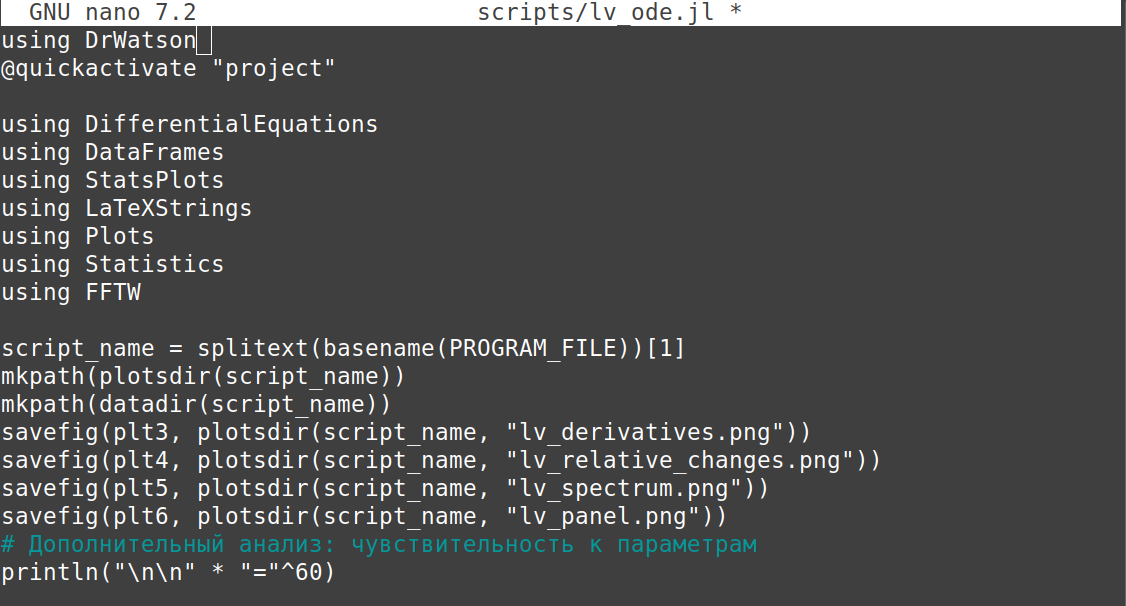
\includegraphics[width=0.7\textwidth,height=\textheight]{image/pic9.png}

}

\caption{\label{fig-008}Код из лабораторного руководства}

\end{figure}%

Я преобразую код в литературный стиль(рис.9)

\begin{figure}

\centering{

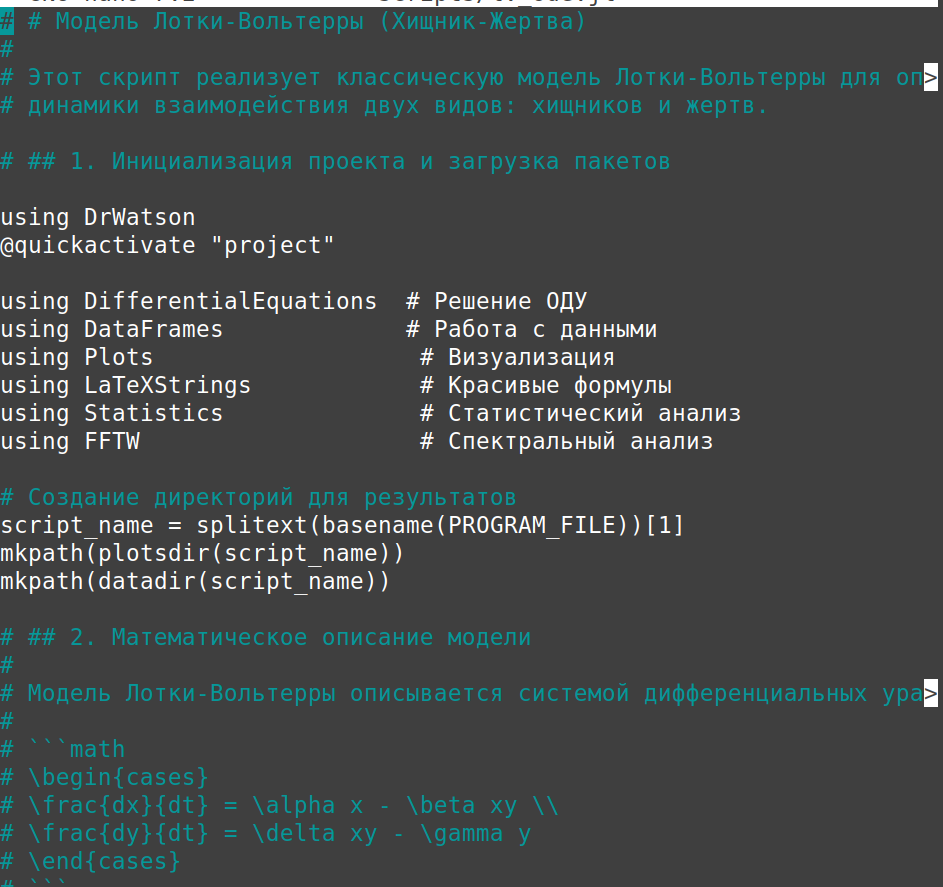
\includegraphics[width=0.7\textwidth,height=\textheight]{image/pic13.png}

}

\caption{\label{fig-009}Код в литературном стиле}

\end{figure}%

После этого я запускаю код, чтобы проверить, работает ли он без ошибок,
и это так(рис.10)

\begin{figure}

\centering{

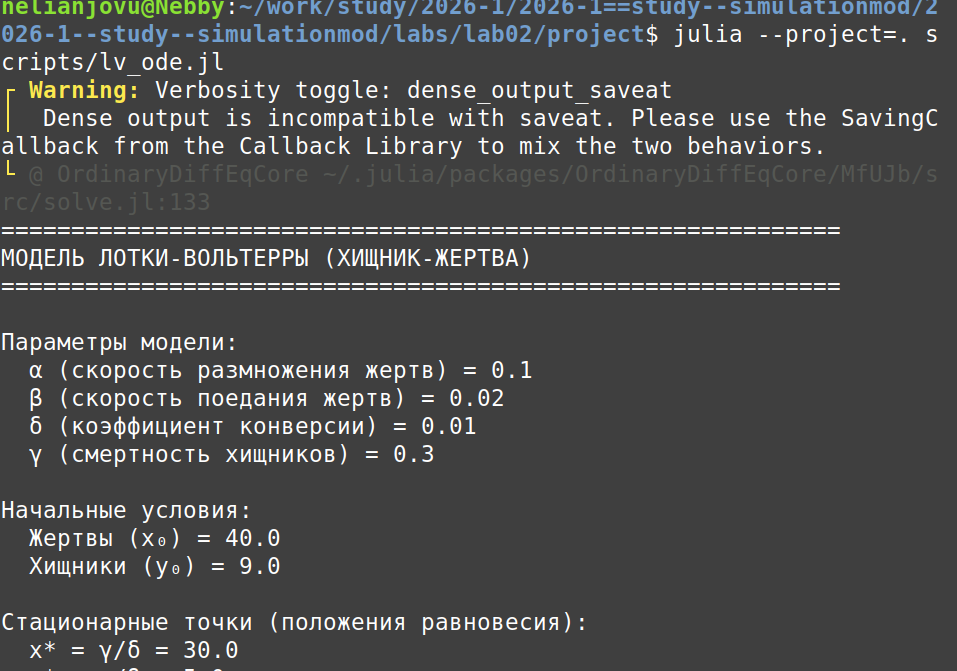
\includegraphics[width=0.7\textwidth,height=\textheight]{image/pic14.png}

}

\caption{\label{fig-010}запуск кода}

\end{figure}%

Затем я создаю файл jupyter notebook, используя файл tangle, который мы
создали ранее. Я запускаю код из файла jupyter notebook, чтобы
убедиться, что он работает без ошибок(рис.11)

\begin{figure}

\centering{

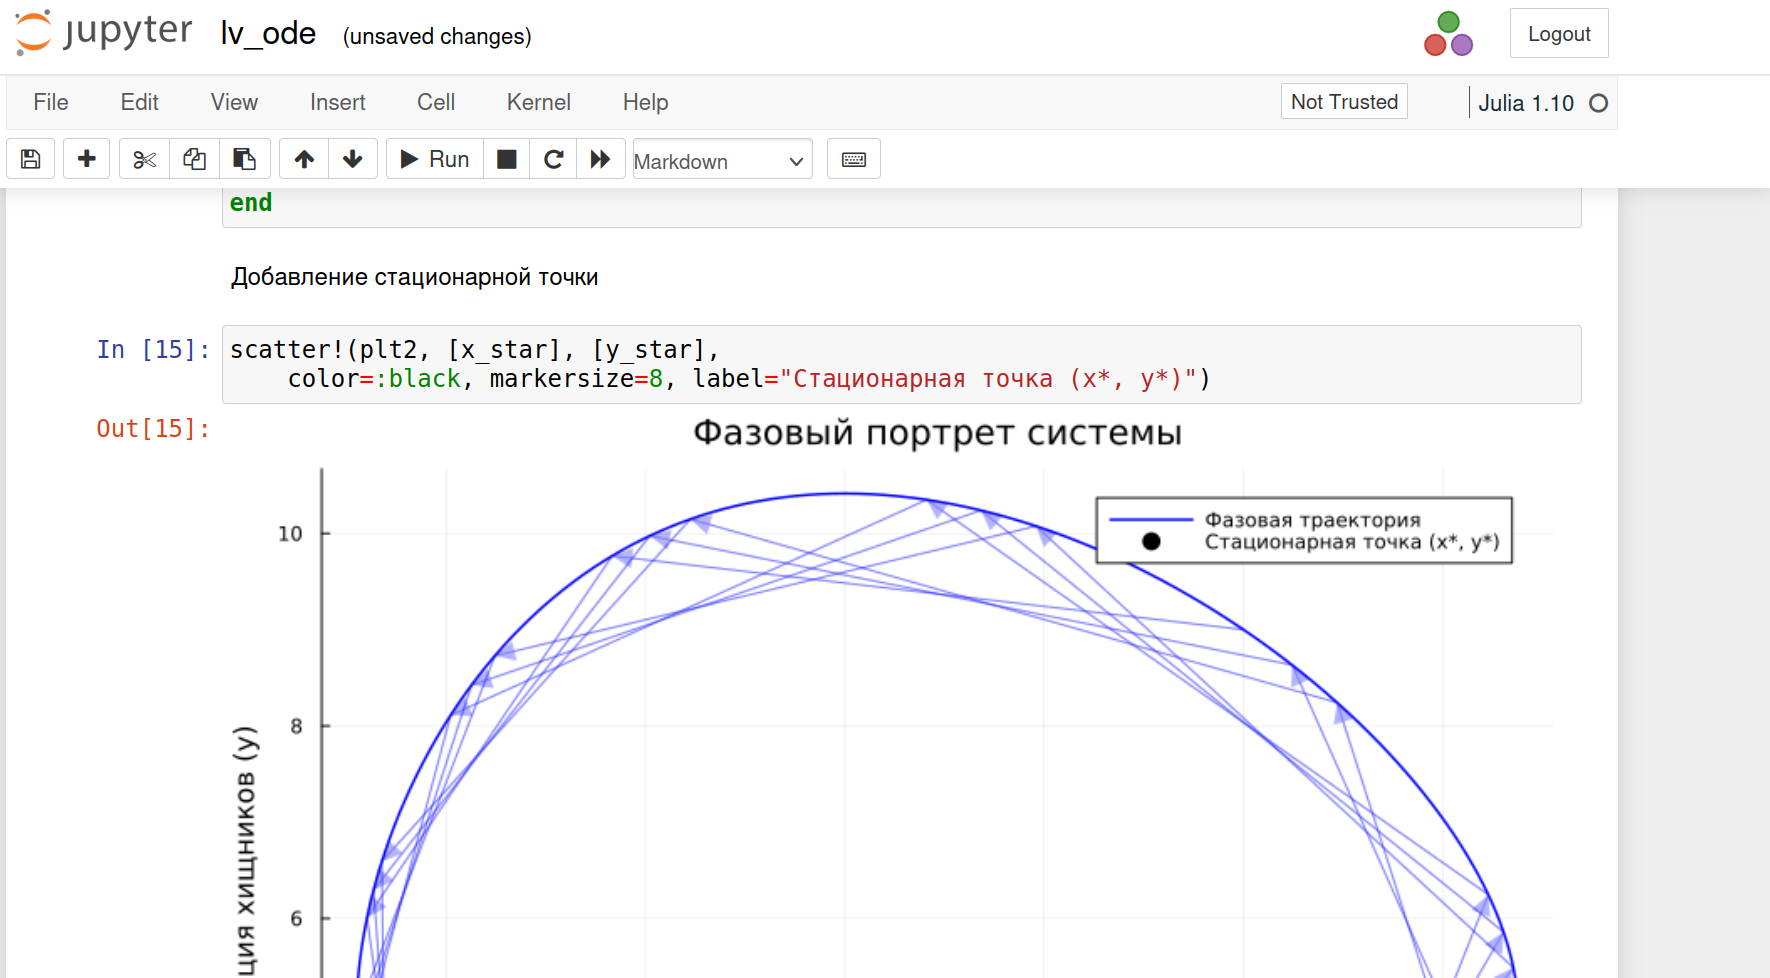
\includegraphics[width=0.7\textwidth,height=\textheight]{image/pic15.png}

}

\caption{\label{fig-011}запуск кода из jupyter notebook}

\end{figure}%

Я добавляю в код расчет для набора параметров в литературном стиле,
чтобы поэкспериментировать с ним(рис.12)

\begin{figure}

\centering{

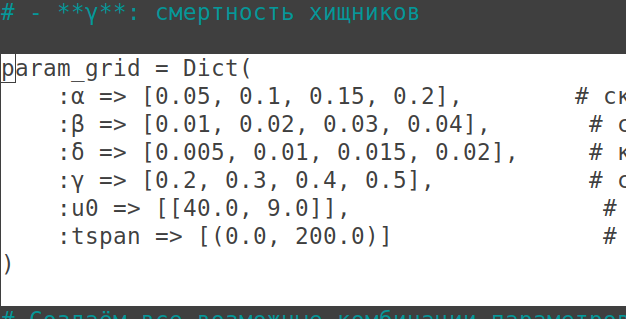
\includegraphics[width=0.7\textwidth,height=\textheight]{image/pic25.png}

}

\caption{\label{fig-012}добавление кода}

\end{figure}%

После этого я запускаю код, чтобы проверить, работает ли он без ошибок,
и это так. Наблюдения: Когда γ (смертность хищников) высокая,
равновесная численность жертв (x\emph{) увеличивается. Когда δ
(коэффициент конверсии) низкий, колебания становятся больше. Когда α
(рождаемость жертв) низкая, система все еще может иметь большие
колебания, если другие параметры позволяют. Когда β (поедание жертв)
высокий, равновесная численность хищников (y}) уменьшается.

Затем я создаю файл jupyter notebook, используя файл tangle, который мы
создали ранее. Я запускаю код из файла jupyter notebook, чтобы
убедиться, что он работает без ошибок. (рис.13)

\begin{figure}

\centering{

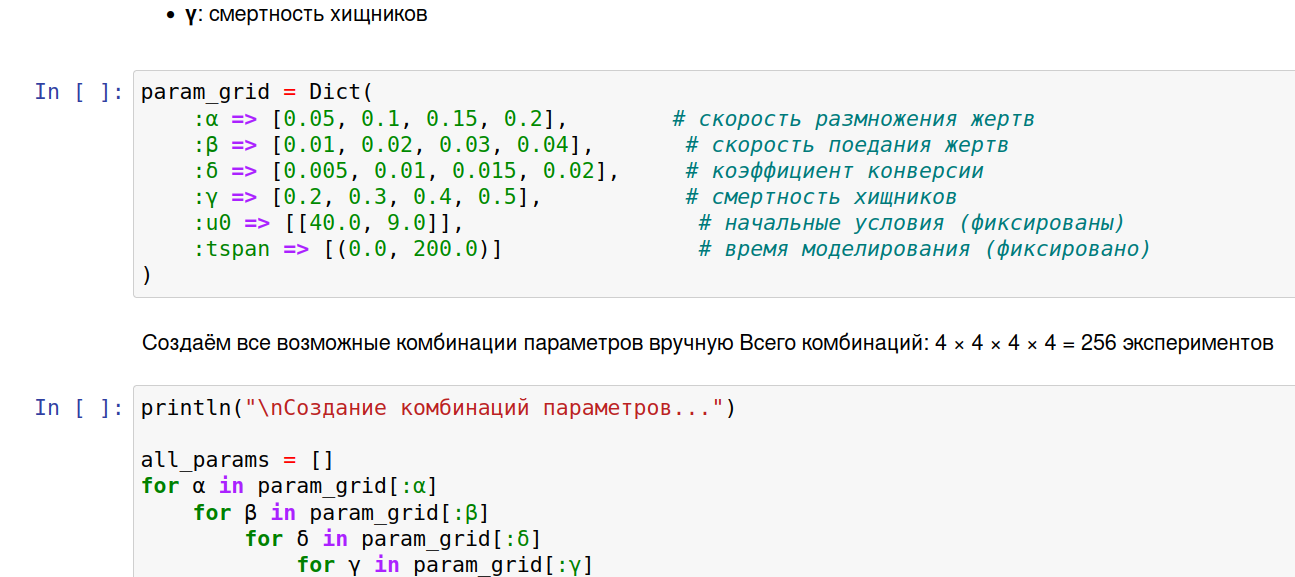
\includegraphics[width=0.7\textwidth,height=\textheight]{image/pic26.png}

}

\caption{\label{fig-013}запуск кода из jupyter notebook}

\end{figure}%

\textbf{\emph{Ниже приведен код, результаты расчетов и графики для кода
в файле lv\_ode.jl.qmd}}

\chapter{Модель Лотки-Вольтерры
(Хищник-Жертва)}\label{ux43cux43eux434ux435ux43bux44c-ux43bux43eux442ux43aux438-ux432ux43eux43bux44cux442ux435ux440ux440ux44b-ux445ux438ux449ux43dux438ux43a-ux436ux435ux440ux442ux432ux430}

Этот скрипт реализует классическую модель Лотки-Вольтерры для описания
динамики взаимодействия двух видов: хищников и жертв.

\textbf{Версия с параметрическим сканированием}

\section{1. Инициализация проекта и загрузка
пакетов}\label{ux438ux43dux438ux446ux438ux430ux43bux438ux437ux430ux446ux438ux44f-ux43fux440ux43eux435ux43aux442ux430-ux438-ux437ux430ux433ux440ux443ux437ux43aux430-ux43fux430ux43aux435ux442ux43eux432-1}

\begin{Shaded}
\begin{Highlighting}[]
\ImportTok{using} \BuiltInTok{DrWatson}
\PreprocessorTok{@quickactivate} \StringTok{"project"}

\ImportTok{using} \BuiltInTok{DifferentialEquations}  \CommentTok{\# Решение ОДУ}
\ImportTok{using} \BuiltInTok{DataFrames}             \CommentTok{\# Работа с данными}
\ImportTok{using} \BuiltInTok{Plots}                   \CommentTok{\# Визуализация}
\ImportTok{using} \BuiltInTok{LaTeXStrings}            \CommentTok{\# Красивые формулы}
\ImportTok{using} \BuiltInTok{Statistics}              \CommentTok{\# Статистический анализ}
\ImportTok{using} \BuiltInTok{FFTW}                    \CommentTok{\# Спектральный анализ}
\ImportTok{using} \BuiltInTok{JLD2}                    \CommentTok{\# Для сохранения данных}
\ImportTok{using} \BuiltInTok{CSV}                     \CommentTok{\# Для сохранения в CSV}
\end{Highlighting}
\end{Shaded}

\begin{verbatim}
┌ Warning: DrWatson could not find find a project file by recursively checking given `dir` and its parents. Returning `nothing` instead.
│ (given dir: /home/nelianjovu)
└ @ DrWatson ~/.julia/packages/DrWatson/2QF5p/src/project_setup.jl:84
\end{verbatim}

Создание директорий для результатов

\begin{Shaded}
\begin{Highlighting}[]
\NormalTok{script\_name }\OperatorTok{=} \FunctionTok{splitext}\NormalTok{(}\FunctionTok{basename}\NormalTok{(}\ConstantTok{PROGRAM\_FILE}\NormalTok{))[}\FloatTok{1}\NormalTok{]}
\FunctionTok{mkpath}\NormalTok{(}\FunctionTok{plotsdir}\NormalTok{(script\_name))}
\FunctionTok{mkpath}\NormalTok{(}\FunctionTok{datadir}\NormalTok{(script\_name))}
\end{Highlighting}
\end{Shaded}

\begin{verbatim}
"/home/nelianjovu/work/study/2026-1/2026-1==study--simulationmod/2026-1--study--simulationmod/labs/lab02/project/data"
\end{verbatim}

\section{2. Математическое описание
модели}\label{ux43cux430ux442ux435ux43cux430ux442ux438ux447ux435ux441ux43aux43eux435-ux43eux43fux438ux441ux430ux43dux438ux435-ux43cux43eux434ux435ux43bux438}

Модель Лотки-Вольтерры описывается системой дифференциальных уравнений:

\begin{Shaded}
\begin{Highlighting}[]
\NormalTok{\textbackslash{}begin\{cases\}}
\NormalTok{\textbackslash{}frac\{dx\}\{dt\} = \textbackslash{}alpha x {-} \textbackslash{}beta xy \textbackslash{}\textbackslash{}}
\NormalTok{\textbackslash{}frac\{dy\}\{dt\} = \textbackslash{}delta xy {-} \textbackslash{}gamma y}
\NormalTok{\textbackslash{}end\{cases\}}
\end{Highlighting}
\end{Shaded}

где: - \textbf{x} - популяция жертв (например, зайцы) - \textbf{y} -
популяция хищников (например, лисы) - \textbf{α} - естественный прирост
жертв (в отсутствие хищников) - \textbf{β} - коэффициент поедания жертв
хищниками - \textbf{δ} - коэффициент прироста хищников за счет поедания
жертв - \textbf{γ} - естественная смертность хищников (в отсутствие
жертв)

\begin{Shaded}
\begin{Highlighting}[]
\KeywordTok{function} \FunctionTok{lotka\_volterra!}\NormalTok{(du, u, p, t)}
\NormalTok{    x, y }\OperatorTok{=}\NormalTok{ u}
\NormalTok{    α, β, δ, γ }\OperatorTok{=}\NormalTok{ p}

    \PreprocessorTok{@inbounds} \ControlFlowTok{begin}
\NormalTok{        du[}\FloatTok{1}\NormalTok{] }\OperatorTok{=}\NormalTok{ α}\OperatorTok{*}\NormalTok{x }\OperatorTok{{-}}\NormalTok{ β}\OperatorTok{*}\NormalTok{x}\OperatorTok{*}\NormalTok{y  }\CommentTok{\# изменение популяции жертв}
\NormalTok{        du[}\FloatTok{2}\NormalTok{] }\OperatorTok{=}\NormalTok{ δ}\OperatorTok{*}\NormalTok{x}\OperatorTok{*}\NormalTok{y }\OperatorTok{{-}}\NormalTok{ γ}\OperatorTok{*}\NormalTok{y   }\CommentTok{\# изменение популяции хищников}
    \ControlFlowTok{end}
    \ConstantTok{nothing}
\KeywordTok{end}
\end{Highlighting}
\end{Shaded}

\begin{verbatim}
lotka_volterra! (generic function with 1 method)
\end{verbatim}

\section{3. Базовые параметры модели (один
эксперимент)}\label{ux431ux430ux437ux43eux432ux44bux435-ux43fux430ux440ux430ux43cux435ux442ux440ux44b-ux43cux43eux434ux435ux43bux438-ux43eux434ux438ux43d-ux44dux43aux441ux43fux435ux440ux438ux43cux435ux43dux442}

Используем классические параметры из литературы: - \textbf{α = 0.1} -
скорость размножения жертв - \textbf{β = 0.02} - скорость поедания жертв
- \textbf{δ = 0.01} - коэффициент конверсии пищи в потомство - \textbf{γ
= 0.3} - смертность хищников

Начальные условия: - \textbf{x₀ = 40} - начальная популяция жертв -
\textbf{y₀ = 9} - начальная популяция хищников

Время моделирования: \textbf{200 единиц}

\begin{Shaded}
\begin{Highlighting}[]
\NormalTok{p\_lv }\OperatorTok{=}\NormalTok{ [}\FloatTok{0.1}\NormalTok{, }\FloatTok{0.02}\NormalTok{, }\FloatTok{0.01}\NormalTok{, }\FloatTok{0.3}\NormalTok{]}
\NormalTok{u0\_lv }\OperatorTok{=}\NormalTok{ [}\FloatTok{40.0}\NormalTok{, }\FloatTok{9.0}\NormalTok{]}
\NormalTok{tspan\_lv }\OperatorTok{=}\NormalTok{ (}\FloatTok{0.0}\NormalTok{, }\FloatTok{200.0}\NormalTok{)}
\NormalTok{dt\_lv }\OperatorTok{=} \FloatTok{0.01}
\end{Highlighting}
\end{Shaded}

\begin{verbatim}
0.01
\end{verbatim}

\section{4. Численное решение системы (базовый
эксперимент)}\label{ux447ux438ux441ux43bux435ux43dux43dux43eux435-ux440ux435ux448ux435ux43dux438ux435-ux441ux438ux441ux442ux435ux43cux44b-ux431ux430ux437ux43eux432ux44bux439-ux44dux43aux441ux43fux435ux440ux438ux43cux435ux43dux442}

\begin{Shaded}
\begin{Highlighting}[]
\NormalTok{prob\_lv }\OperatorTok{=} \FunctionTok{ODEProblem}\NormalTok{(lotka\_volterra!, u0\_lv, tspan\_lv, p\_lv)}
\NormalTok{sol\_lv }\OperatorTok{=} \FunctionTok{solve}\NormalTok{(prob\_lv,}
\NormalTok{    dt }\OperatorTok{=}\NormalTok{ dt\_lv,}
    \FunctionTok{Tsit5}\NormalTok{(),}
\NormalTok{    reltol}\OperatorTok{=}\FloatTok{1e{-}8}\NormalTok{,}
\NormalTok{    abstol}\OperatorTok{=}\FloatTok{1e{-}10}\NormalTok{,}
\NormalTok{    saveat}\OperatorTok{=}\FloatTok{0.1}\NormalTok{,}
\NormalTok{    dense}\OperatorTok{=}\ConstantTok{true}
\NormalTok{)}
\end{Highlighting}
\end{Shaded}

\begin{verbatim}
┌ Warning: Verbosity toggle: dense_output_saveat 
│  Dense output is incompatible with saveat. Please use the SavingCallback from the Callback Library to mix the two behaviors.
└ @ OrdinaryDiffEqCore ~/.julia/packages/OrdinaryDiffEqCore/MfUJb/src/solve.jl:133
\end{verbatim}

\begin{verbatim}
retcode: Success
Interpolation: specialized 4th order "free" interpolation
t: 2001-element Vector{Float64}:
   0.0
   0.1
   0.2
   0.3
   0.4
   0.5
   0.6
   0.7
   0.8
   0.9
   1.0
   1.1
   1.2
   ⋮
 198.9
 199.0
 199.1
 199.2
 199.3
 199.4
 199.5
 199.6
 199.7
 199.8
 199.9
 200.0
u: 2001-element Vector{Vector{Float64}}:
 [40.0, 9.0]
 [39.67773201890384, 9.088990237207637]
 [39.35113789503168, 9.175882726306998]
 [39.02053587808482, 9.260562174341326]
 [38.68624820281499, 9.342916311942016]
 [38.34860018759226, 9.422836265415746]
 [38.007919320045765, 9.500216918706203]
 [37.664534369328166, 9.57495725033006]
 [37.31877446654823, 9.646960666854818]
 [36.970968217678404, 9.716135308317776]
 [36.62144287329975, 9.78239432138995]
 [36.27052336512251, 9.845656154267314]
 [35.91853163311434, 9.905844751305578]
 ⋮
 [17.889675634214175, 5.712401894068308]
 [17.865436242318786, 5.643570483722319]
 [17.8436734538774, 5.5754402198920205]
 [17.82435314492936, 5.5080193185068556]
 [17.807442037033802, 5.441315154551656]
 [17.79290768632072, 5.375334300040312]
 [17.780718473179366, 5.310082577777455]
 [17.770843588540256, 5.24556508481179]
 [17.76325301314867, 5.1817862454809696]
 [17.75791751745931, 5.118749811721094]
 [17.754808657966603, 5.05645887359248]
 [17.75389874795975, 4.994915937053494]
\end{verbatim}

\section{5. Подготовка данных для
анализа}\label{ux43fux43eux434ux433ux43eux442ux43eux432ux43aux430-ux434ux430ux43dux43dux44bux445-ux434ux43bux44f-ux430ux43dux430ux43bux438ux437ux430}

\begin{Shaded}
\begin{Highlighting}[]
\NormalTok{df\_lv }\OperatorTok{=} \FunctionTok{DataFrame}\NormalTok{()}
\NormalTok{df\_lv[!, }\OperatorTok{:}\NormalTok{t] }\OperatorTok{=}\NormalTok{ sol\_lv.t}
\NormalTok{df\_lv[!, }\OperatorTok{:}\NormalTok{prey] }\OperatorTok{=}\NormalTok{ [u[}\FloatTok{1}\NormalTok{] for u }\KeywordTok{in}\NormalTok{ sol\_lv.u]}
\NormalTok{df\_lv[!, }\OperatorTok{:}\NormalTok{predator] }\OperatorTok{=}\NormalTok{ [u[}\FloatTok{2}\NormalTok{] for u }\KeywordTok{in}\NormalTok{ sol\_lv.u]}
\end{Highlighting}
\end{Shaded}

\begin{verbatim}
2001-element Vector{Float64}:
 9.0
 9.088990237207637
 9.175882726306998
 9.260562174341326
 9.342916311942016
 9.422836265415746
 9.500216918706203
 9.57495725033006
 9.646960666854818
 9.716135308317776
 9.78239432138995
 9.845656154267314
 9.905844751305578
 ⋮
 5.712401894068308
 5.643570483722319
 5.5754402198920205
 5.5080193185068556
 5.441315154551656
 5.375334300040312
 5.310082577777455
 5.24556508481179
 5.1817862454809696
 5.118749811721094
 5.05645887359248
 4.994915937053494
\end{verbatim}

Расчет производных для анализа скоростей изменения

\begin{Shaded}
\begin{Highlighting}[]
\NormalTok{df\_lv[!, }\OperatorTok{:}\NormalTok{dprey\_dt] }\OperatorTok{=}\NormalTok{ p\_lv[}\FloatTok{1}\NormalTok{] }\OperatorTok{.*}\NormalTok{ df\_lv.prey }\OperatorTok{.{-}}\NormalTok{ p\_lv[}\FloatTok{2}\NormalTok{] }\OperatorTok{.*}\NormalTok{ df\_lv.prey }\OperatorTok{.*}\NormalTok{ df\_lv.predator}
\NormalTok{df\_lv[!, }\OperatorTok{:}\NormalTok{dpredator\_dt] }\OperatorTok{=}\NormalTok{ p\_lv[}\FloatTok{3}\NormalTok{] }\OperatorTok{.*}\NormalTok{ df\_lv.prey }\OperatorTok{.*}\NormalTok{ df\_lv.predator }\OperatorTok{.{-}}\NormalTok{ p\_lv[}\FloatTok{4}\NormalTok{] }\OperatorTok{.*}\NormalTok{ df\_lv.predator}
\end{Highlighting}
\end{Shaded}

\begin{verbatim}
2001-element Vector{Float64}:
  0.9000000000000004
  0.8796081183812872
  0.8580494468233599
  0.8353523334488115
  0.8115489002365717
  0.7866749261310106
  0.7607697060793308
  0.7338758893000268
  0.706039294083721
  0.6773087043294623
  0.6477356516317538
  0.6173741696029542
  0.5862805551332175
  ⋮
 -0.6917903984489653
 -0.6848226585569628
 -0.6777687195139299
 -0.6706369809304631
 -0.6634355041663743
 -0.6561720201747868
 -0.6488539394852814
 -0.6414883588865548
 -0.6340820722589693
 -0.6266415740257927
 -0.6191730642026256
 -0.6116824631058659
\end{verbatim}

Расчет относительных изменений (в процентах)

\begin{Shaded}
\begin{Highlighting}[]
\NormalTok{df\_lv[!, }\OperatorTok{:}\NormalTok{prey\_pct\_change] }\OperatorTok{=}\NormalTok{ df\_lv.dprey\_dt }\OperatorTok{./}\NormalTok{ df\_lv.prey }\OperatorTok{.*} \FloatTok{100}
\NormalTok{df\_lv[!, }\OperatorTok{:}\NormalTok{predator\_pct\_change] }\OperatorTok{=}\NormalTok{ df\_lv.dpredator\_dt }\OperatorTok{./}\NormalTok{ df\_lv.predator }\OperatorTok{.*} \FloatTok{100}
\end{Highlighting}
\end{Shaded}

\begin{verbatim}
2001-element Vector{Float64}:
  10.000000000000004
   9.677732018903836
   9.351137895031682
   9.020535878084827
   8.686248202814987
   8.348600187592261
   8.007919320045769
   7.664534369328169
   7.318774466548226
   6.97096821767841
   6.621442873299746
   6.27052336512251
   5.918531633114344
   ⋮
 -12.110324365785825
 -12.134563757681214
 -12.1563265461226
 -12.175646855070637
 -12.192557962966195
 -12.207092313679277
 -12.219281526820632
 -12.229156411459744
 -12.236746986851331
 -12.24208248254069
 -12.245191342033394
 -12.246101252040251
\end{verbatim}

\section{6. Вывод информации о
модели}\label{ux432ux44bux432ux43eux434-ux438ux43dux444ux43eux440ux43cux430ux446ux438ux438-ux43e-ux43cux43eux434ux435ux43bux438}

\begin{Shaded}
\begin{Highlighting}[]
\FunctionTok{println}\NormalTok{(}\StringTok{"="}\OperatorTok{\^{}}\FloatTok{60}\NormalTok{)}
\FunctionTok{println}\NormalTok{(}\StringTok{"МОДЕЛЬ ЛОТКИ{-}ВОЛЬТЕРРЫ (ХИЩНИК{-}ЖЕРТВА)"}\NormalTok{)}
\FunctionTok{println}\NormalTok{(}\StringTok{"="}\OperatorTok{\^{}}\FloatTok{60}\NormalTok{)}
\FunctionTok{println}\NormalTok{(}\StringTok{"}\SpecialCharTok{\textbackslash{}n}\StringTok{Параметры модели:"}\NormalTok{)}
\FunctionTok{println}\NormalTok{(}\StringTok{"  α (скорость размножения жертв) = "}\NormalTok{, p\_lv[}\FloatTok{1}\NormalTok{])}
\FunctionTok{println}\NormalTok{(}\StringTok{"  β (скорость поедания жертв) = "}\NormalTok{, p\_lv[}\FloatTok{2}\NormalTok{])}
\FunctionTok{println}\NormalTok{(}\StringTok{"  δ (коэффициент конверсии) = "}\NormalTok{, p\_lv[}\FloatTok{3}\NormalTok{])}
\FunctionTok{println}\NormalTok{(}\StringTok{"  γ (смертность хищников) = "}\NormalTok{, p\_lv[}\FloatTok{4}\NormalTok{])}
\FunctionTok{println}\NormalTok{(}\StringTok{"}\SpecialCharTok{\textbackslash{}n}\StringTok{Начальные условия:"}\NormalTok{)}
\FunctionTok{println}\NormalTok{(}\StringTok{"  Жертвы (x₀) = "}\NormalTok{, u0\_lv[}\FloatTok{1}\NormalTok{])}
\FunctionTok{println}\NormalTok{(}\StringTok{"  Хищники (y₀) = "}\NormalTok{, u0\_lv[}\FloatTok{2}\NormalTok{])}
\end{Highlighting}
\end{Shaded}

\begin{verbatim}
============================================================
МОДЕЛЬ ЛОТКИ-ВОЛЬТЕРРЫ (ХИЩНИК-ЖЕРТВА)
============================================================

Параметры модели:
  α (скорость размножения жертв) = 0.1
  β (скорость поедания жертв) = 0.02
  δ (коэффициент конверсии) = 0.01
  γ (смертность хищников) = 0.3

Начальные условия:
  Жертвы (x₀) = 40.0
  Хищники (y₀) = 9.0
\end{verbatim}

\section{7. Стационарные точки (положения
равновесия)}\label{ux441ux442ux430ux446ux438ux43eux43dux430ux440ux43dux44bux435-ux442ux43eux447ux43aux438-ux43fux43eux43bux43eux436ux435ux43dux438ux44f-ux440ux430ux432ux43dux43eux432ux435ux441ux438ux44f}

\begin{Shaded}
\begin{Highlighting}[]
\NormalTok{x\^{}* = \textbackslash{}frac\{\textbackslash{}gamma\}\{\textbackslash{}delta\}, \textbackslash{}quad y\^{}* = \textbackslash{}frac\{\textbackslash{}alpha\}\{\textbackslash{}beta\}}
\end{Highlighting}
\end{Shaded}

\begin{Shaded}
\begin{Highlighting}[]
\NormalTok{x\_star }\OperatorTok{=}\NormalTok{ p\_lv[}\FloatTok{4}\NormalTok{] }\OperatorTok{/}\NormalTok{ p\_lv[}\FloatTok{3}\NormalTok{]}
\NormalTok{y\_star }\OperatorTok{=}\NormalTok{ p\_lv[}\FloatTok{1}\NormalTok{] }\OperatorTok{/}\NormalTok{ p\_lv[}\FloatTok{2}\NormalTok{]}

\FunctionTok{println}\NormalTok{(}\StringTok{"}\SpecialCharTok{\textbackslash{}n}\StringTok{Стационарные точки (положения равновесия):"}\NormalTok{)}
\FunctionTok{println}\NormalTok{(}\StringTok{"  x* = γ/δ = "}\NormalTok{, }\FunctionTok{round}\NormalTok{(x\_star, digits}\OperatorTok{=}\FloatTok{3}\NormalTok{))}
\FunctionTok{println}\NormalTok{(}\StringTok{"  y* = α/β = "}\NormalTok{, }\FunctionTok{round}\NormalTok{(y\_star, digits}\OperatorTok{=}\FloatTok{3}\NormalTok{))}
\end{Highlighting}
\end{Shaded}

\begin{verbatim}

Стационарные точки (положения равновесия):
  x* = γ/δ = 30.0
  y* = α/β = 5.0
\end{verbatim}

============================================================ 8.
ВИЗУАЛИЗАЦИЯ БАЗОВОГО ЭКСПЕРИМЕНТА
============================================================

\section{8.1 График 1: Динамика популяций во
времени}\label{ux433ux440ux430ux444ux438ux43a-1-ux434ux438ux43dux430ux43cux438ux43aux430-ux43fux43eux43fux443ux43bux44fux446ux438ux439-ux432ux43e-ux432ux440ux435ux43cux435ux43dux438}

Отображает изменение численности жертв и хищников с течением времени.

\begin{Shaded}
\begin{Highlighting}[]
\NormalTok{plt1 }\OperatorTok{=} \FunctionTok{plot}\NormalTok{(df\_lv.t, [df\_lv.prey df\_lv.predator],}
\NormalTok{    label}\OperatorTok{=}\NormalTok{[L}\StringTok{"Жертвы (x)"}\NormalTok{ L}\StringTok{"Хищники (y)"}\NormalTok{],}
\NormalTok{    xlabel}\OperatorTok{=}\StringTok{"Время"}\NormalTok{,}
\NormalTok{    ylabel}\OperatorTok{=}\StringTok{"Популяция"}\NormalTok{,}
\NormalTok{    title}\OperatorTok{=}\StringTok{"Модель Лотки{-}Вольтерры: Динамика популяций"}\NormalTok{,}
\NormalTok{    linewidth}\OperatorTok{=}\FloatTok{2}\NormalTok{,}
\NormalTok{    legend}\OperatorTok{=:}\NormalTok{topright,}
\NormalTok{    grid}\OperatorTok{=}\ConstantTok{true}\NormalTok{,}
\NormalTok{    size}\OperatorTok{=}\NormalTok{(}\FloatTok{900}\NormalTok{, }\FloatTok{500}\NormalTok{),}
\NormalTok{    color}\OperatorTok{=}\NormalTok{[}\OperatorTok{:}\NormalTok{green }\OperatorTok{:}\NormalTok{red])}
\end{Highlighting}
\end{Shaded}

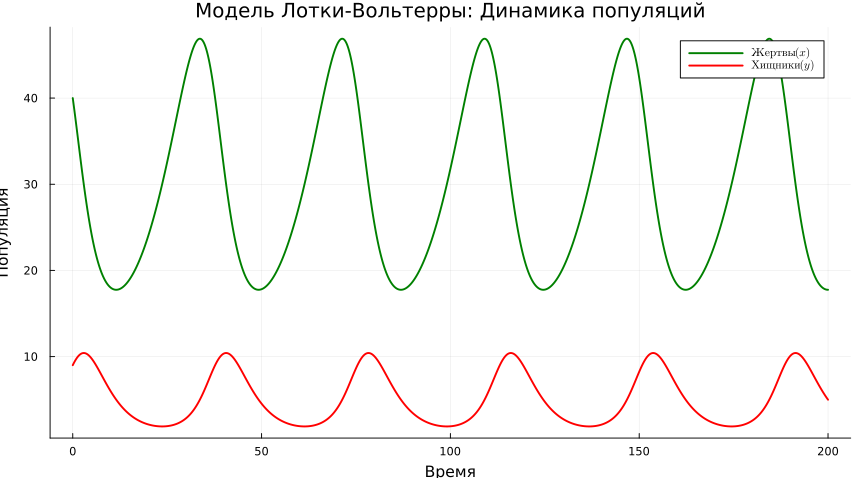
\includegraphics{simmod-lab02-report (Нелиа Нджову)_files/figure-pdf/cell-49-output-1.png}

Добавление стационарных уровней

\begin{Shaded}
\begin{Highlighting}[]
\FunctionTok{hline!}\NormalTok{(plt1, [x\_star], color}\OperatorTok{=:}\NormalTok{green, linestyle}\OperatorTok{=:}\NormalTok{dash, alpha}\OperatorTok{=}\FloatTok{0.5}\NormalTok{,}
\NormalTok{       label}\OperatorTok{=}\StringTok{"x* (равновесие жертв)"}\NormalTok{)}
\FunctionTok{hline!}\NormalTok{(plt1, [y\_star], color}\OperatorTok{=:}\NormalTok{red, linestyle}\OperatorTok{=:}\NormalTok{dash, alpha}\OperatorTok{=}\FloatTok{0.5}\NormalTok{,}
\NormalTok{       label}\OperatorTok{=}\StringTok{"y* (равновесие хищников)"}\NormalTok{)}
\end{Highlighting}
\end{Shaded}

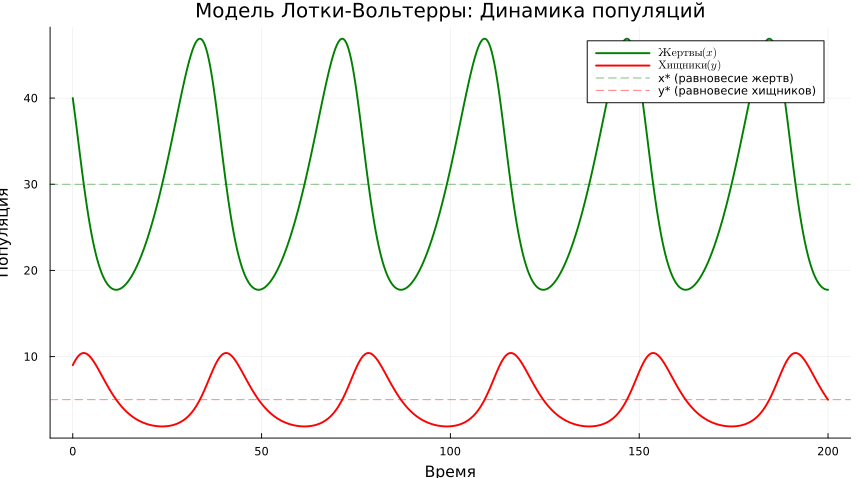
\includegraphics{simmod-lab02-report (Нелиа Нджову)_files/figure-pdf/cell-50-output-1.png}

\section{8.2 График 2: Фазовый портрет (хищники vs
жертвы)}\label{ux433ux440ux430ux444ux438ux43a-2-ux444ux430ux437ux43eux432ux44bux439-ux43fux43eux440ux442ux440ux435ux442-ux445ux438ux449ux43dux438ux43aux438-vs-ux436ux435ux440ux442ux432ux44b}

Показывает зависимость численности хищников от численности жертв.
Замкнутые траектории указывают на циклический характер системы.

\begin{Shaded}
\begin{Highlighting}[]
\NormalTok{plt2 }\OperatorTok{=} \FunctionTok{plot}\NormalTok{(df\_lv.prey, df\_lv.predator,}
\NormalTok{    label}\OperatorTok{=}\StringTok{"Фазовая траектория"}\NormalTok{,}
\NormalTok{    xlabel}\OperatorTok{=}\StringTok{"Популяция жертв (x)"}\NormalTok{,}
\NormalTok{    ylabel}\OperatorTok{=}\StringTok{"Популяция хищников (y)"}\NormalTok{,}
\NormalTok{    title}\OperatorTok{=}\StringTok{"Фазовый портрет системы"}\NormalTok{,}
\NormalTok{    color}\OperatorTok{=:}\NormalTok{blue,}
\NormalTok{    linewidth}\OperatorTok{=}\FloatTok{1.5}\NormalTok{,}
\NormalTok{    grid}\OperatorTok{=}\ConstantTok{true}\NormalTok{,}
\NormalTok{    size}\OperatorTok{=}\NormalTok{(}\FloatTok{800}\NormalTok{, }\FloatTok{600}\NormalTok{),}
\NormalTok{    legend}\OperatorTok{=:}\NormalTok{topright)}
\end{Highlighting}
\end{Shaded}

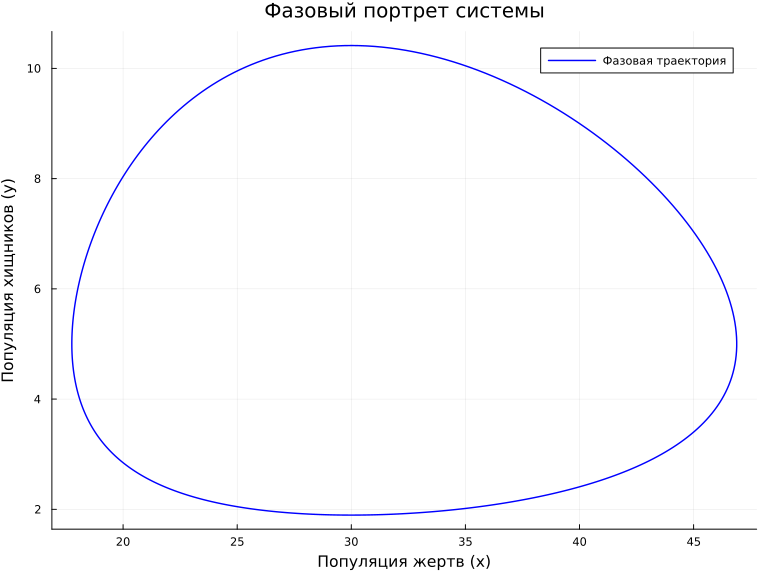
\includegraphics{simmod-lab02-report (Нелиа Нджову)_files/figure-pdf/cell-51-output-1.png}

Добавление стрелок направления на фазовом портрете

\begin{Shaded}
\begin{Highlighting}[]
\NormalTok{step }\OperatorTok{=} \FloatTok{50}
\ControlFlowTok{for}\NormalTok{ i }\KeywordTok{in} \FloatTok{1}\OperatorTok{:}\NormalTok{step}\OperatorTok{:}\FunctionTok{length}\NormalTok{(df\_lv.prey)}\OperatorTok{{-}}\NormalTok{step}
    \FunctionTok{plot!}\NormalTok{(plt2,}
\NormalTok{        [df\_lv.prey[i], df\_lv.prey[i}\OperatorTok{+}\NormalTok{step]],}
\NormalTok{        [df\_lv.predator[i], df\_lv.predator[i}\OperatorTok{+}\NormalTok{step]],}
\NormalTok{        arrow}\OperatorTok{=:}\NormalTok{closed, color}\OperatorTok{=:}\NormalTok{blue, alpha}\OperatorTok{=}\FloatTok{0.3}\NormalTok{, label}\OperatorTok{=}\ConstantTok{false}\NormalTok{)}
\ControlFlowTok{end}
\end{Highlighting}
\end{Shaded}

Добавление стационарной точки

\begin{Shaded}
\begin{Highlighting}[]
\FunctionTok{scatter!}\NormalTok{(plt2, [x\_star], [y\_star],}
\NormalTok{    color}\OperatorTok{=:}\NormalTok{black, markersize}\OperatorTok{=}\FloatTok{8}\NormalTok{, label}\OperatorTok{=}\StringTok{"Стационарная точка (x*, y*)"}\NormalTok{)}
\end{Highlighting}
\end{Shaded}

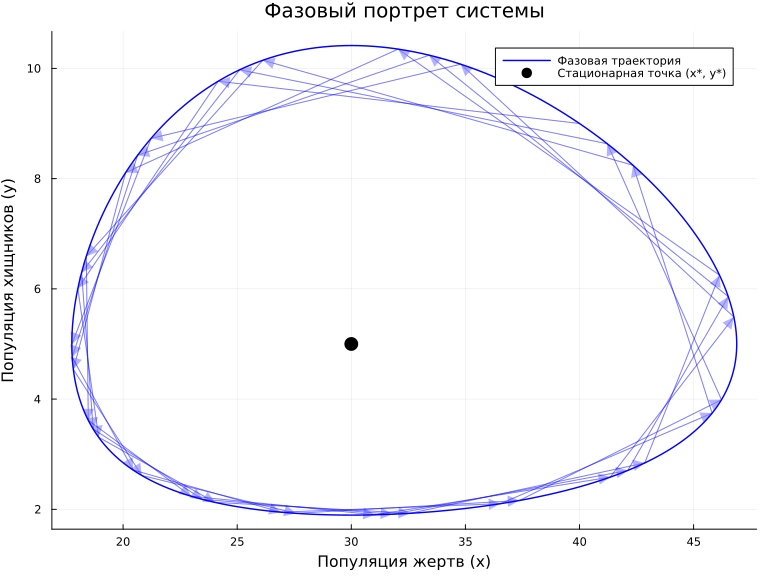
\includegraphics{simmod-lab02-report (Нелиа Нджову)_files/figure-pdf/cell-53-output-1.png}

Изоклины (линии нулевого роста)

\begin{Shaded}
\begin{Highlighting}[]
\NormalTok{x\_range }\OperatorTok{=} \FunctionTok{LinRange}\NormalTok{(}\FloatTok{0}\NormalTok{, }\FunctionTok{maximum}\NormalTok{(df\_lv.prey)}\OperatorTok{*}\FloatTok{1.1}\NormalTok{, }\FloatTok{100}\NormalTok{)}
\NormalTok{y\_nullcline }\OperatorTok{=}\NormalTok{ p\_lv[}\FloatTok{1}\NormalTok{] }\OperatorTok{./}\NormalTok{ (p\_lv[}\FloatTok{2}\NormalTok{] }\OperatorTok{.*}\NormalTok{ x\_range)  }\CommentTok{\# dy/dt = 0}
\FunctionTok{plot!}\NormalTok{(plt2, x\_range, y\_nullcline,}
\NormalTok{    color}\OperatorTok{=:}\NormalTok{red, linestyle}\OperatorTok{=:}\NormalTok{dash, linewidth}\OperatorTok{=}\FloatTok{1.5}\NormalTok{, label}\OperatorTok{=}\StringTok{"Изоклина хищников (dy/dt=0)"}\NormalTok{)}

\NormalTok{y\_range }\OperatorTok{=} \FunctionTok{LinRange}\NormalTok{(}\FloatTok{0}\NormalTok{, }\FunctionTok{maximum}\NormalTok{(df\_lv.predator)}\OperatorTok{*}\FloatTok{1.1}\NormalTok{, }\FloatTok{100}\NormalTok{)}
\NormalTok{x\_nullcline }\OperatorTok{=}\NormalTok{ p\_lv[}\FloatTok{4}\NormalTok{] }\OperatorTok{./}\NormalTok{ (p\_lv[}\FloatTok{3}\NormalTok{] }\OperatorTok{.*} \FunctionTok{ones}\NormalTok{(}\FunctionTok{length}\NormalTok{(y\_range)))  }\CommentTok{\# dx/dt = 0}
\FunctionTok{plot!}\NormalTok{(plt2, x\_nullcline, y\_range,}
\NormalTok{    color}\OperatorTok{=:}\NormalTok{green, linestyle}\OperatorTok{=:}\NormalTok{dash, linewidth}\OperatorTok{=}\FloatTok{1.5}\NormalTok{, label}\OperatorTok{=}\StringTok{"Изоклина жертв (dx/dt=0)"}\NormalTok{)}
\end{Highlighting}
\end{Shaded}

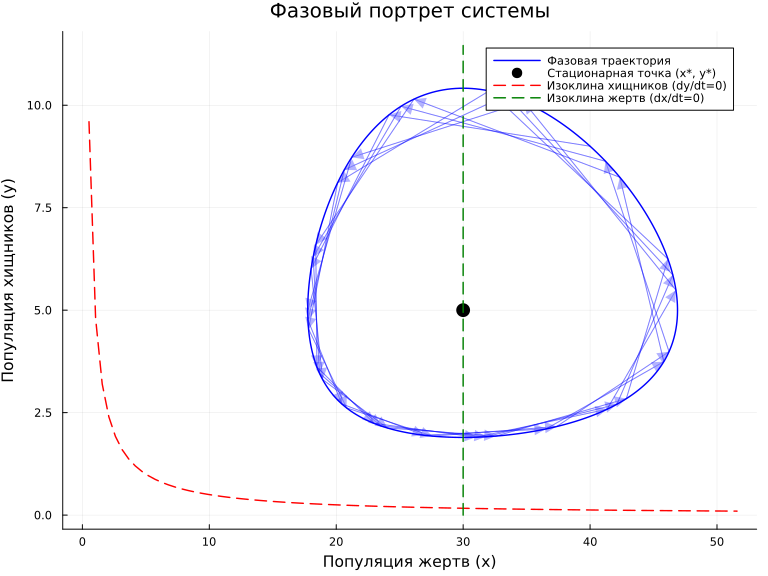
\includegraphics{simmod-lab02-report (Нелиа Нджову)_files/figure-pdf/cell-54-output-1.png}

\section{8.3 График 3: Производные (скорости
изменения)}\label{ux433ux440ux430ux444ux438ux43a-3-ux43fux440ux43eux438ux437ux432ux43eux434ux43dux44bux435-ux441ux43aux43eux440ux43eux441ux442ux438-ux438ux437ux43cux435ux43dux435ux43dux438ux44f}

\begin{Shaded}
\begin{Highlighting}[]
\NormalTok{plt3 }\OperatorTok{=} \FunctionTok{plot}\NormalTok{(df\_lv.t, [df\_lv.dprey\_dt df\_lv.dpredator\_dt],}
\NormalTok{    label}\OperatorTok{=}\NormalTok{[L}\StringTok{"dx/dt"}\NormalTok{ L}\StringTok{"dy/dt"}\NormalTok{],}
\NormalTok{    xlabel}\OperatorTok{=}\StringTok{"Время"}\NormalTok{,}
\NormalTok{    ylabel}\OperatorTok{=}\StringTok{"Скорость изменения"}\NormalTok{,}
\NormalTok{    title}\OperatorTok{=}\StringTok{"Производные популяций"}\NormalTok{,}
\NormalTok{    linewidth}\OperatorTok{=}\FloatTok{1.5}\NormalTok{,}
\NormalTok{    legend}\OperatorTok{=:}\NormalTok{topright,}
\NormalTok{    grid}\OperatorTok{=}\ConstantTok{true}\NormalTok{,}
\NormalTok{    size}\OperatorTok{=}\NormalTok{(}\FloatTok{900}\NormalTok{, }\FloatTok{400}\NormalTok{),}
\NormalTok{    color}\OperatorTok{=}\NormalTok{[}\OperatorTok{:}\NormalTok{green }\OperatorTok{:}\NormalTok{red])}

\FunctionTok{hline!}\NormalTok{(plt3, [}\FloatTok{0}\NormalTok{], color}\OperatorTok{=:}\NormalTok{black, linestyle}\OperatorTok{=:}\NormalTok{solid, alpha}\OperatorTok{=}\FloatTok{0.3}\NormalTok{, label}\OperatorTok{=}\ConstantTok{false}\NormalTok{)}
\end{Highlighting}
\end{Shaded}

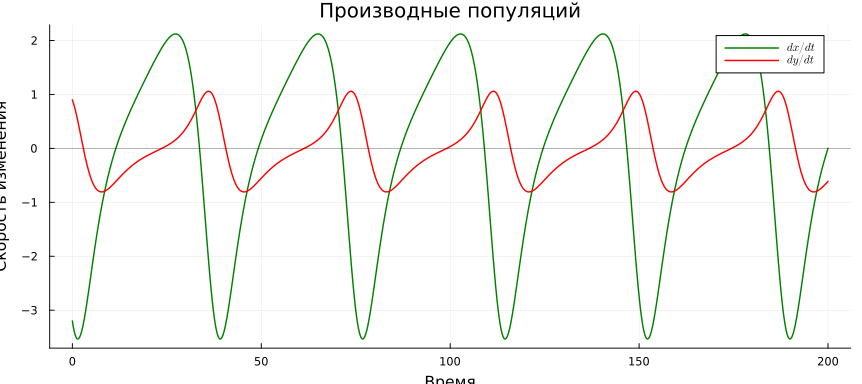
\includegraphics{simmod-lab02-report (Нелиа Нджову)_files/figure-pdf/cell-55-output-1.png}

\section{8.4 График 4: Относительные изменения (в
процентах)}\label{ux433ux440ux430ux444ux438ux43a-4-ux43eux442ux43dux43eux441ux438ux442ux435ux43bux44cux43dux44bux435-ux438ux437ux43cux435ux43dux435ux43dux438ux44f-ux432-ux43fux440ux43eux446ux435ux43dux442ux430ux445}

\begin{Shaded}
\begin{Highlighting}[]
\NormalTok{plt4 }\OperatorTok{=} \FunctionTok{plot}\NormalTok{(df\_lv.t, [df\_lv.prey\_pct\_change df\_lv.predator\_pct\_change],}
\NormalTok{    label}\OperatorTok{=}\NormalTok{[L}\StringTok{"dx/dt / x (\textbackslash{}\%)"}\NormalTok{ L}\StringTok{"dy/dt / y (\textbackslash{}\%)"}\NormalTok{],}
\NormalTok{    xlabel}\OperatorTok{=}\StringTok{"Время"}\NormalTok{,}
\NormalTok{    ylabel}\OperatorTok{=}\StringTok{"Относительное изменение, \%"}\NormalTok{,}
\NormalTok{    title}\OperatorTok{=}\StringTok{"Относительные темпы роста"}\NormalTok{,}
\NormalTok{    linewidth}\OperatorTok{=}\FloatTok{1.5}\NormalTok{,}
\NormalTok{    legend}\OperatorTok{=:}\NormalTok{topright,}
\NormalTok{    grid}\OperatorTok{=}\ConstantTok{true}\NormalTok{,}
\NormalTok{    size}\OperatorTok{=}\NormalTok{(}\FloatTok{900}\NormalTok{, }\FloatTok{400}\NormalTok{),}
\NormalTok{    color}\OperatorTok{=}\NormalTok{[}\OperatorTok{:}\NormalTok{green }\OperatorTok{:}\NormalTok{red])}
\end{Highlighting}
\end{Shaded}

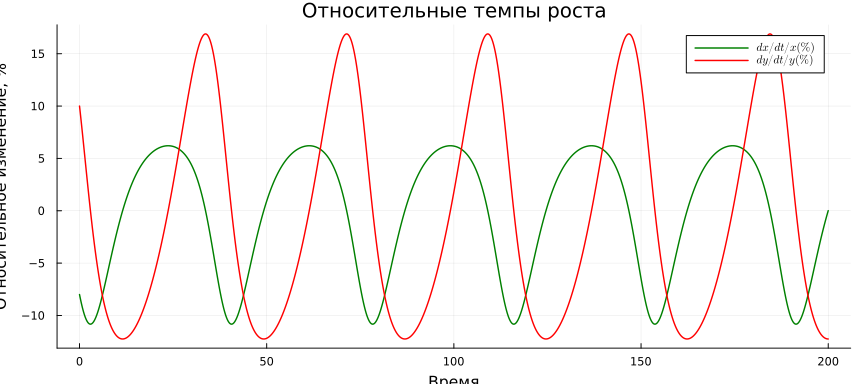
\includegraphics{simmod-lab02-report (Нелиа Нджову)_files/figure-pdf/cell-56-output-1.png}

\section{8.5 График 5: Спектральный анализ
(FFT)}\label{ux433ux440ux430ux444ux438ux43a-5-ux441ux43fux435ux43aux442ux440ux430ux43bux44cux43dux44bux439-ux430ux43dux430ux43bux438ux437-fft}

Функция для вычисления быстрого преобразования Фурье

\begin{Shaded}
\begin{Highlighting}[]
\KeywordTok{function} \FunctionTok{compute\_fft}\NormalTok{(signal, dt)}
\NormalTok{    n }\OperatorTok{=} \FunctionTok{length}\NormalTok{(signal)}
\NormalTok{    spectrum }\OperatorTok{=} \FunctionTok{abs}\NormalTok{.(}\FunctionTok{rfft}\NormalTok{(signal }\OperatorTok{.{-}} \FunctionTok{mean}\NormalTok{(signal)))}
\NormalTok{    freq }\OperatorTok{=} \FunctionTok{rfftfreq}\NormalTok{(n, }\FloatTok{1}\OperatorTok{/}\NormalTok{dt)}
    \ControlFlowTok{return}\NormalTok{ freq, spectrum}
\KeywordTok{end}
\end{Highlighting}
\end{Shaded}

\begin{verbatim}
compute_fft (generic function with 1 method)
\end{verbatim}

Вычисление периодов колебаний

\begin{Shaded}
\begin{Highlighting}[]
\NormalTok{freq\_prey, spectrum\_prey }\OperatorTok{=} \FunctionTok{compute\_fft}\NormalTok{(df\_lv.prey, dt\_lv)}
\NormalTok{freq\_predator, spectrum\_predator }\OperatorTok{=} \FunctionTok{compute\_fft}\NormalTok{(df\_lv.predator, dt\_lv)}

\NormalTok{plt5 }\OperatorTok{=} \FunctionTok{plot}\NormalTok{(freq\_prey, [spectrum\_prey spectrum\_predator],}
\NormalTok{    label}\OperatorTok{=}\NormalTok{[L}\StringTok{"Жертвы (x)"}\NormalTok{ L}\StringTok{"Хищники (y)"}\NormalTok{],}
\NormalTok{    xlabel}\OperatorTok{=}\StringTok{"Частота"}\NormalTok{,}
\NormalTok{    ylabel}\OperatorTok{=}\StringTok{"Амплитуда"}\NormalTok{,}
\NormalTok{    title}\OperatorTok{=}\StringTok{"Спектральный анализ (Фурье)"}\NormalTok{,}
\NormalTok{    linewidth}\OperatorTok{=}\FloatTok{1.5}\NormalTok{,}
\NormalTok{    xscale}\OperatorTok{=:}\NormalTok{log10,}
\NormalTok{    yscale}\OperatorTok{=:}\NormalTok{log10,}
\NormalTok{    legend}\OperatorTok{=:}\NormalTok{topright,}
\NormalTok{    grid}\OperatorTok{=}\ConstantTok{true}\NormalTok{,}
\NormalTok{    size}\OperatorTok{=}\NormalTok{(}\FloatTok{800}\NormalTok{, }\FloatTok{400}\NormalTok{),}
\NormalTok{    color}\OperatorTok{=}\NormalTok{[}\OperatorTok{:}\NormalTok{green }\OperatorTok{:}\NormalTok{red])}
\end{Highlighting}
\end{Shaded}

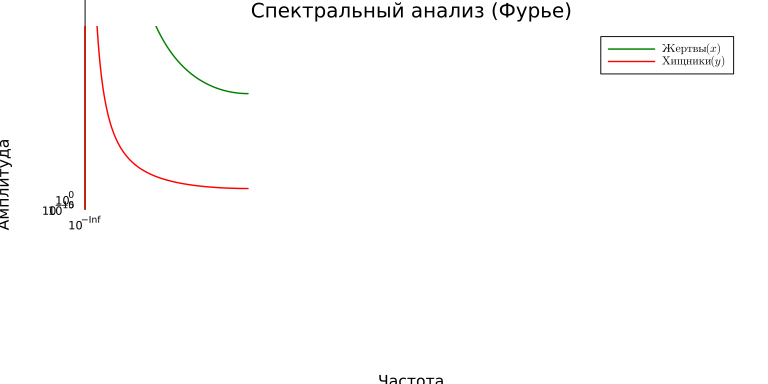
\includegraphics{simmod-lab02-report (Нелиа Нджову)_files/figure-pdf/cell-58-output-1.png}

\begin{verbatim}
┌ Warning: No strict ticks found
└ @ PlotUtils ~/.julia/packages/PlotUtils/HX80C/src/ticks.jl:194
┌ Warning: No strict ticks found
└ @ PlotUtils ~/.julia/packages/PlotUtils/HX80C/src/ticks.jl:194
┌ Warning: Invalid negative or zero value 0.0 found at series index 1 for log10 based xscale
└ @ Plots ~/.julia/packages/Plots/GIume/src/utils.jl:105
┌ Warning: Invalid negative or zero value 0.0 found at series index 1 for log10 based xscale
└ @ Plots ~/.julia/packages/Plots/GIume/src/utils.jl:105
\end{verbatim}

Нахождение доминирующих частот

\begin{Shaded}
\begin{Highlighting}[]
\ControlFlowTok{if} \FunctionTok{length}\NormalTok{(spectrum\_prey) }\OperatorTok{\textgreater{}} \FloatTok{0}
\NormalTok{    idx\_prey }\OperatorTok{=} \FunctionTok{argmax}\NormalTok{(spectrum\_prey[}\FloatTok{2}\OperatorTok{:}\KeywordTok{end}\NormalTok{]) }\OperatorTok{+} \FloatTok{1}  \CommentTok{\# пропускаем нулевую частоту}
\NormalTok{    dominant\_freq\_prey }\OperatorTok{=}\NormalTok{ freq\_prey[idx\_prey]}
\NormalTok{    period\_prey }\OperatorTok{=} \FloatTok{1}\OperatorTok{/}\NormalTok{dominant\_freq\_prey}

    \FunctionTok{println}\NormalTok{(}\StringTok{"}\SpecialCharTok{\textbackslash{}n}\StringTok{Спектральный анализ:"}\NormalTok{)}
    \FunctionTok{println}\NormalTok{(}\StringTok{"  Доминирующая частота колебаний жертв: "}\NormalTok{, }\FunctionTok{round}\NormalTok{(dominant\_freq\_prey, digits}\OperatorTok{=}\FloatTok{4}\NormalTok{))}
    \FunctionTok{println}\NormalTok{(}\StringTok{"  Период колебаний жертв: "}\NormalTok{, }\FunctionTok{round}\NormalTok{(period\_prey, digits}\OperatorTok{=}\FloatTok{2}\NormalTok{), }\StringTok{" ед. времени"}\NormalTok{)}
\ControlFlowTok{end}
\end{Highlighting}
\end{Shaded}

\begin{verbatim}

Спектральный анализ:
  Доминирующая частота колебаний жертв: 0.2499
  Период колебаний жертв: 4.0 ед. времени
\end{verbatim}

\section{8.6 График 6: Компактная панель всех
графиков}\label{ux433ux440ux430ux444ux438ux43a-6-ux43aux43eux43cux43fux430ux43aux442ux43dux430ux44f-ux43fux430ux43dux435ux43bux44c-ux432ux441ux435ux445-ux433ux440ux430ux444ux438ux43aux43eux432}

\begin{Shaded}
\begin{Highlighting}[]
\NormalTok{plt6 }\OperatorTok{=} \FunctionTok{plot}\NormalTok{(layout}\OperatorTok{=}\NormalTok{(}\FloatTok{3}\NormalTok{, }\FloatTok{2}\NormalTok{), size}\OperatorTok{=}\NormalTok{(}\FloatTok{1200}\NormalTok{, }\FloatTok{900}\NormalTok{))}

\FunctionTok{plot!}\NormalTok{(plt6[}\FloatTok{1}\NormalTok{], df\_lv.t, df\_lv.prey, label}\OperatorTok{=}\NormalTok{L}\StringTok{"x(t)"}\NormalTok{, color}\OperatorTok{=:}\NormalTok{green, linewidth}\OperatorTok{=}\FloatTok{2}\NormalTok{,}
\NormalTok{    title}\OperatorTok{=}\StringTok{"Популяция жертв"}\NormalTok{, grid}\OperatorTok{=}\ConstantTok{true}\NormalTok{)}
\FunctionTok{plot!}\NormalTok{(plt6[}\FloatTok{2}\NormalTok{], df\_lv.t, df\_lv.predator, label}\OperatorTok{=}\NormalTok{L}\StringTok{"y(t)"}\NormalTok{, color}\OperatorTok{=:}\NormalTok{red, linewidth}\OperatorTok{=}\FloatTok{2}\NormalTok{,}
\NormalTok{    title}\OperatorTok{=}\StringTok{"Популяция хищников"}\NormalTok{, grid}\OperatorTok{=}\ConstantTok{true}\NormalTok{)}
\FunctionTok{plot!}\NormalTok{(plt6[}\FloatTok{3}\NormalTok{], df\_lv.prey, df\_lv.predator, label}\OperatorTok{=}\ConstantTok{false}\NormalTok{, color}\OperatorTok{=:}\NormalTok{blue, linewidth}\OperatorTok{=}\FloatTok{1.5}\NormalTok{,}
\NormalTok{    title}\OperatorTok{=}\StringTok{"Фазовый портрет"}\NormalTok{, xlabel}\OperatorTok{=}\NormalTok{L}\StringTok{"x"}\NormalTok{, ylabel}\OperatorTok{=}\NormalTok{L}\StringTok{"y"}\NormalTok{, grid}\OperatorTok{=}\ConstantTok{true}\NormalTok{)}
\FunctionTok{scatter!}\NormalTok{(plt6[}\FloatTok{3}\NormalTok{], [x\_star], [y\_star], color}\OperatorTok{=:}\NormalTok{black, markersize}\OperatorTok{=}\FloatTok{5}\NormalTok{, label}\OperatorTok{=}\StringTok{"(x*, y*)"}\NormalTok{)}
\FunctionTok{plot!}\NormalTok{(plt6[}\FloatTok{4}\NormalTok{], df\_lv.t, [df\_lv.dprey\_dt df\_lv.dpredator\_dt],}
\NormalTok{    label}\OperatorTok{=}\NormalTok{[L}\StringTok{"dx/dt"}\NormalTok{ L}\StringTok{"dy/dt"}\NormalTok{], color}\OperatorTok{=}\NormalTok{[}\OperatorTok{:}\NormalTok{green }\OperatorTok{:}\NormalTok{red], linewidth}\OperatorTok{=}\FloatTok{1.5}\NormalTok{,}
\NormalTok{    title}\OperatorTok{=}\StringTok{"Скорости изменения"}\NormalTok{, grid}\OperatorTok{=}\ConstantTok{true}\NormalTok{, legend}\OperatorTok{=:}\NormalTok{topright)}
\FunctionTok{plot!}\NormalTok{(plt6[}\FloatTok{5}\NormalTok{], freq\_prey, spectrum\_prey, label}\OperatorTok{=}\NormalTok{L}\StringTok{"x"}\NormalTok{, color}\OperatorTok{=:}\NormalTok{green, linewidth}\OperatorTok{=}\FloatTok{1.5}\NormalTok{,}
\NormalTok{    title}\OperatorTok{=}\StringTok{"Спектр жертв"}\NormalTok{, xscale}\OperatorTok{=:}\NormalTok{log10, yscale}\OperatorTok{=:}\NormalTok{log10, grid}\OperatorTok{=}\ConstantTok{true}\NormalTok{)}
\FunctionTok{plot!}\NormalTok{(plt6[}\FloatTok{6}\NormalTok{], df\_lv.t, [df\_lv.prey\_pct\_change df\_lv.predator\_pct\_change],}
\NormalTok{    label}\OperatorTok{=}\NormalTok{[L}\StringTok{"dx/x"}\NormalTok{ L}\StringTok{"dy/y"}\NormalTok{], color}\OperatorTok{=}\NormalTok{[}\OperatorTok{:}\NormalTok{green }\OperatorTok{:}\NormalTok{red], linewidth}\OperatorTok{=}\FloatTok{1.5}\NormalTok{,}
\NormalTok{    title}\OperatorTok{=}\StringTok{"Относительные изменения"}\NormalTok{, grid}\OperatorTok{=}\ConstantTok{true}\NormalTok{, legend}\OperatorTok{=:}\NormalTok{topright)}
\end{Highlighting}
\end{Shaded}

\begin{verbatim}
┌ Warning: No strict ticks found
└ @ PlotUtils ~/.julia/packages/PlotUtils/HX80C/src/ticks.jl:194
┌ Warning: No strict ticks found
└ @ PlotUtils ~/.julia/packages/PlotUtils/HX80C/src/ticks.jl:194
┌ Warning: Invalid negative or zero value 0.0 found at series index 1 for log10 based xscale
└ @ Plots ~/.julia/packages/Plots/GIume/src/utils.jl:105
\end{verbatim}

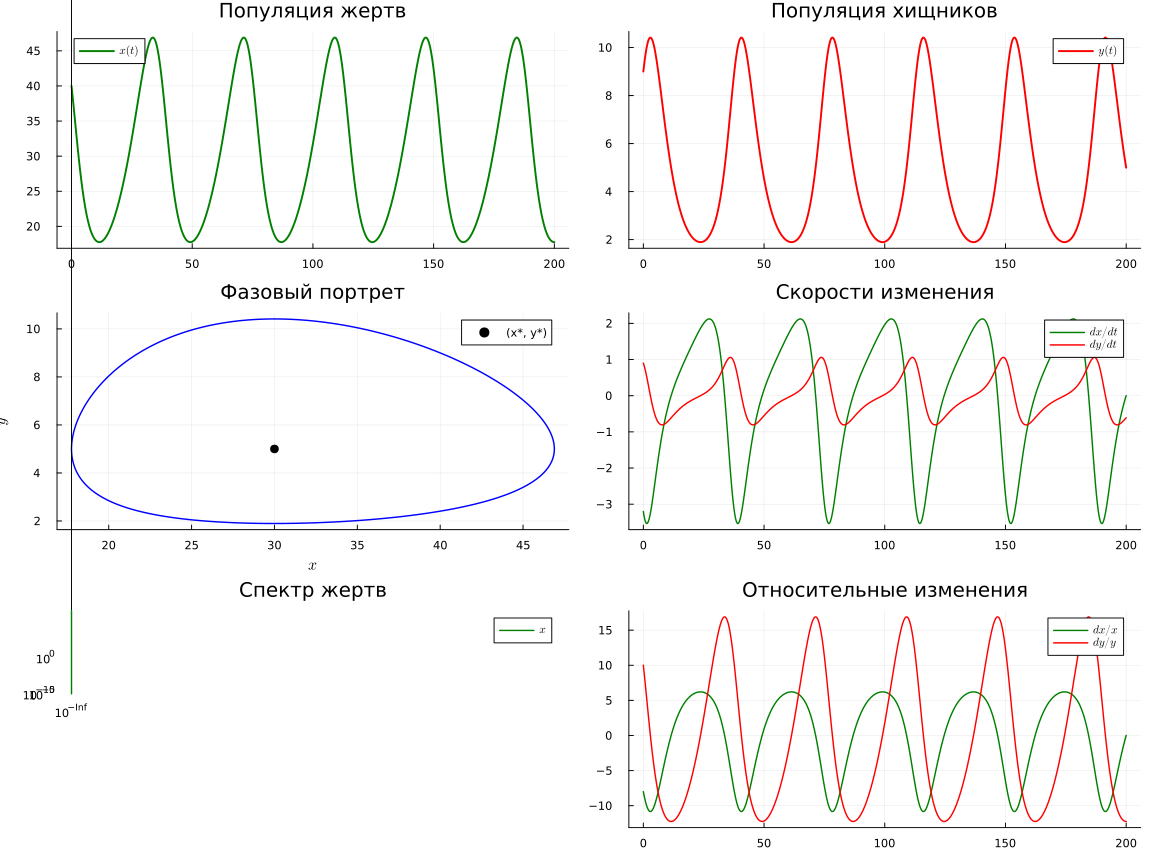
\includegraphics{simmod-lab02-report (Нелиа Нджову)_files/figure-pdf/cell-60-output-2.png}

============================================================ 9. АНАЛИЗ
БАЗОВОГО ЭКСПЕРИМЕНТА
============================================================

\begin{Shaded}
\begin{Highlighting}[]
\FunctionTok{println}\NormalTok{(}\StringTok{"}\SpecialCharTok{\textbackslash{}n}\StringTok{"} \OperatorTok{*} \StringTok{"="}\OperatorTok{\^{}}\FloatTok{60}\NormalTok{)}
\FunctionTok{println}\NormalTok{(}\StringTok{"АНАЛИЗ БАЗОВОГО ЭКСПЕРИМЕНТА"}\NormalTok{)}
\FunctionTok{println}\NormalTok{(}\StringTok{"="}\OperatorTok{\^{}}\FloatTok{60}\NormalTok{)}

\FunctionTok{println}\NormalTok{(}\StringTok{"}\SpecialCharTok{\textbackslash{}n}\StringTok{Основные статистики:"}\NormalTok{)}
\FunctionTok{println}\NormalTok{(}\StringTok{"  Жертвы: min = }\SpecialCharTok{$}\NormalTok{(}\FunctionTok{round}\NormalTok{(}\FunctionTok{minimum}\NormalTok{(df\_lv.prey), digits}\OperatorTok{=}\FloatTok{2}\NormalTok{))}\StringTok{, "} \OperatorTok{*}
        \StringTok{"max = }\SpecialCharTok{$}\NormalTok{(}\FunctionTok{round}\NormalTok{(}\FunctionTok{maximum}\NormalTok{(df\_lv.prey), digits}\OperatorTok{=}\FloatTok{2}\NormalTok{))}\StringTok{, "} \OperatorTok{*}
        \StringTok{"mean = }\SpecialCharTok{$}\NormalTok{(}\FunctionTok{round}\NormalTok{(}\FunctionTok{mean}\NormalTok{(df\_lv.prey), digits}\OperatorTok{=}\FloatTok{2}\NormalTok{))}\StringTok{"}\NormalTok{)}
\FunctionTok{println}\NormalTok{(}\StringTok{"  Хищники: min = }\SpecialCharTok{$}\NormalTok{(}\FunctionTok{round}\NormalTok{(}\FunctionTok{minimum}\NormalTok{(df\_lv.predator), digits}\OperatorTok{=}\FloatTok{2}\NormalTok{))}\StringTok{, "} \OperatorTok{*}
        \StringTok{"max = }\SpecialCharTok{$}\NormalTok{(}\FunctionTok{round}\NormalTok{(}\FunctionTok{maximum}\NormalTok{(df\_lv.predator), digits}\OperatorTok{=}\FloatTok{2}\NormalTok{))}\StringTok{, "} \OperatorTok{*}
        \StringTok{"mean = }\SpecialCharTok{$}\NormalTok{(}\FunctionTok{round}\NormalTok{(}\FunctionTok{mean}\NormalTok{(df\_lv.predator), digits}\OperatorTok{=}\FloatTok{2}\NormalTok{))}\StringTok{"}\NormalTok{)}
\end{Highlighting}
\end{Shaded}

\begin{verbatim}

============================================================
АНАЛИЗ БАЗОВОГО ЭКСПЕРИМЕНТА
============================================================

Основные статистики:
  Жертвы: min = 17.75, max = 46.89, mean = 29.71
  Хищники: min = 1.9, max = 10.41, mean = 5.2
\end{verbatim}

\section{9.1 Анализ
колебаний}\label{ux430ux43dux430ux43bux438ux437-ux43aux43eux43bux435ux431ux430ux43dux438ux439}

Функция для поиска первого пика в сигнале

\begin{Shaded}
\begin{Highlighting}[]
\KeywordTok{function} \FunctionTok{find\_first\_peak}\NormalTok{(signal, time)}
    \ControlFlowTok{for}\NormalTok{ i }\KeywordTok{in} \FloatTok{2}\OperatorTok{:}\FunctionTok{length}\NormalTok{(signal)}\OperatorTok{{-}}\FloatTok{1}
        \ControlFlowTok{if}\NormalTok{ signal[i] }\OperatorTok{\textgreater{}}\NormalTok{ signal[i}\OperatorTok{{-}}\FloatTok{1}\NormalTok{] }\OperatorTok{\&\&}\NormalTok{ signal[i] }\OperatorTok{\textgreater{}}\NormalTok{ signal[i}\OperatorTok{+}\FloatTok{1}\NormalTok{]}
            \ControlFlowTok{return}\NormalTok{ time[i], signal[i]}
        \ControlFlowTok{end}
    \ControlFlowTok{end}
    \ControlFlowTok{return} \ConstantTok{NaN}\NormalTok{, }\ConstantTok{NaN}
\KeywordTok{end}

\NormalTok{peak\_time\_prey, peak\_value\_prey }\OperatorTok{=} \FunctionTok{find\_first\_peak}\NormalTok{(df\_lv.prey, df\_lv.t)}
\NormalTok{peak\_time\_predator, peak\_value\_predator }\OperatorTok{=} \FunctionTok{find\_first\_peak}\NormalTok{(df\_lv.predator, df\_lv.t)}

\ControlFlowTok{if}\NormalTok{ !}\FunctionTok{isnan}\NormalTok{(peak\_time\_prey) }\OperatorTok{\&\&}\NormalTok{ !}\FunctionTok{isnan}\NormalTok{(peak\_time\_predator)}
\NormalTok{    phase\_shift }\OperatorTok{=}\NormalTok{ peak\_time\_predator }\OperatorTok{{-}}\NormalTok{ peak\_time\_prey}
    \FunctionTok{println}\NormalTok{(}\StringTok{"}\SpecialCharTok{\textbackslash{}n}\StringTok{Анализ колебаний:"}\NormalTok{)}
    \FunctionTok{println}\NormalTok{(}\StringTok{"  Первый пик жертв: время = }\SpecialCharTok{$}\NormalTok{(}\FunctionTok{round}\NormalTok{(peak\_time\_prey, digits}\OperatorTok{=}\FloatTok{2}\NormalTok{))}\StringTok{, "} \OperatorTok{*}
            \StringTok{"значение = }\SpecialCharTok{$}\NormalTok{(}\FunctionTok{round}\NormalTok{(peak\_value\_prey, digits}\OperatorTok{=}\FloatTok{2}\NormalTok{))}\StringTok{"}\NormalTok{)}
    \FunctionTok{println}\NormalTok{(}\StringTok{"  Первый пик хищников: время = }\SpecialCharTok{$}\NormalTok{(}\FunctionTok{round}\NormalTok{(peak\_time\_predator, digits}\OperatorTok{=}\FloatTok{2}\NormalTok{))}\StringTok{, "} \OperatorTok{*}
            \StringTok{"значение = }\SpecialCharTok{$}\NormalTok{(}\FunctionTok{round}\NormalTok{(peak\_value\_predator, digits}\OperatorTok{=}\FloatTok{2}\NormalTok{))}\StringTok{"}\NormalTok{)}
    \FunctionTok{println}\NormalTok{(}\StringTok{"  Сдвиг фаз (хищники отстают): }\SpecialCharTok{$}\NormalTok{(}\FunctionTok{round}\NormalTok{(phase\_shift, digits}\OperatorTok{=}\FloatTok{2}\NormalTok{))}\StringTok{ ед. времени"}\NormalTok{)}
\ControlFlowTok{end}
\end{Highlighting}
\end{Shaded}

\begin{verbatim}

Анализ колебаний:
  Первый пик жертв: время = 33.7, значение = 46.89
  Первый пик хищников: время = 2.9, значение = 10.41
  Сдвиг фаз (хищники отстают): -30.8 ед. времени
\end{verbatim}

============================================================ 10.
ПАРАМЕТРИЧЕСКОЕ СКАНИРОВАНИЕ
============================================================

\section{10.1 Зачем нужно параметрическое
сканирование?}\label{ux437ux430ux447ux435ux43c-ux43dux443ux436ux43dux43e-ux43fux430ux440ux430ux43cux435ux442ux440ux438ux447ux435ux441ux43aux43eux435-ux441ux43aux430ux43dux438ux440ux43eux432ux430ux43dux438ux435-1}

До сих пор мы рассматривали только один набор параметров. Но как
изменится динамика системы, если: - \textbf{α} (скорость размножения
жертв) будет другой? - \textbf{β} (скорость поедания) изменится? -
\textbf{δ} (эффективность конверсии) будет иной? - \textbf{γ}
(смертность хищников) поменяется?

Чтобы ответить на эти вопросы, проведём \textbf{параметрическое
сканирование} - запустим модель с разными комбинациями параметров и
сравним результаты.

\begin{Shaded}
\begin{Highlighting}[]
\FunctionTok{println}\NormalTok{(}\StringTok{"}\SpecialCharTok{\textbackslash{}n}\StringTok{"} \OperatorTok{*} \StringTok{"="}\OperatorTok{\^{}}\FloatTok{60}\NormalTok{)}
\FunctionTok{println}\NormalTok{(}\StringTok{"ПАРАМЕТРИЧЕСКОЕ СКАНИРОВАНИЕ"}\NormalTok{)}
\FunctionTok{println}\NormalTok{(}\StringTok{"="}\OperatorTok{\^{}}\FloatTok{60}\NormalTok{)}
\end{Highlighting}
\end{Shaded}

\begin{verbatim}

============================================================
ПАРАМЕТРИЧЕСКОЕ СКАНИРОВАНИЕ
============================================================
\end{verbatim}

\section{10.2 Сетка
параметров}\label{ux441ux435ux442ux43aux430-ux43fux430ux440ux430ux43cux435ux442ux440ux43eux432-1}

Создадим словарь с наборами значений для каждого параметра. Мы будем
варьировать 4 параметра: - \textbf{α}: скорость размножения жертв -
\textbf{β}: скорость поедания жертв - \textbf{δ}: коэффициент конверсии
- \textbf{γ}: смертность хищников

\begin{Shaded}
\begin{Highlighting}[]
\NormalTok{param\_grid }\OperatorTok{=} \FunctionTok{Dict}\NormalTok{(}
    \OperatorTok{:}\NormalTok{α }\OperatorTok{=\textgreater{}}\NormalTok{ [}\FloatTok{0.05}\NormalTok{, }\FloatTok{0.1}\NormalTok{, }\FloatTok{0.15}\NormalTok{, }\FloatTok{0.2}\NormalTok{],        }\CommentTok{\# скорость размножения жертв}
    \OperatorTok{:}\NormalTok{β }\OperatorTok{=\textgreater{}}\NormalTok{ [}\FloatTok{0.01}\NormalTok{, }\FloatTok{0.02}\NormalTok{, }\FloatTok{0.03}\NormalTok{, }\FloatTok{0.04}\NormalTok{],       }\CommentTok{\# скорость поедания жертв}
    \OperatorTok{:}\NormalTok{δ }\OperatorTok{=\textgreater{}}\NormalTok{ [}\FloatTok{0.005}\NormalTok{, }\FloatTok{0.01}\NormalTok{, }\FloatTok{0.015}\NormalTok{, }\FloatTok{0.02}\NormalTok{],     }\CommentTok{\# коэффициент конверсии}
    \OperatorTok{:}\NormalTok{γ }\OperatorTok{=\textgreater{}}\NormalTok{ [}\FloatTok{0.2}\NormalTok{, }\FloatTok{0.3}\NormalTok{, }\FloatTok{0.4}\NormalTok{, }\FloatTok{0.5}\NormalTok{],           }\CommentTok{\# смертность хищников}
    \OperatorTok{:}\NormalTok{u0 }\OperatorTok{=\textgreater{}}\NormalTok{ [[}\FloatTok{40.0}\NormalTok{, }\FloatTok{9.0}\NormalTok{]],                  }\CommentTok{\# начальные условия (фиксированы)}
    \OperatorTok{:}\NormalTok{tspan }\OperatorTok{=\textgreater{}}\NormalTok{ [(}\FloatTok{0.0}\NormalTok{, }\FloatTok{200.0}\NormalTok{)]               }\CommentTok{\# время моделирования (фиксировано)}
\NormalTok{)}
\end{Highlighting}
\end{Shaded}

\begin{verbatim}
Dict{Symbol, Vector} with 6 entries:
  :α     => [0.05, 0.1, 0.15, 0.2]
  :γ     => [0.2, 0.3, 0.4, 0.5]
  :u0    => [[40.0, 9.0]]
  :δ     => [0.005, 0.01, 0.015, 0.02]
  :β     => [0.01, 0.02, 0.03, 0.04]
  :tspan => [(0.0, 200.0)]
\end{verbatim}

Создаём все возможные комбинации параметров вручную Всего комбинаций: 4
× 4 × 4 × 4 = 256 экспериментов

\begin{Shaded}
\begin{Highlighting}[]
\FunctionTok{println}\NormalTok{(}\StringTok{"}\SpecialCharTok{\textbackslash{}n}\StringTok{Создание комбинаций параметров..."}\NormalTok{)}

\NormalTok{all\_params }\OperatorTok{=}\NormalTok{ []}
\ControlFlowTok{for}\NormalTok{ α }\KeywordTok{in}\NormalTok{ param\_grid[}\OperatorTok{:}\NormalTok{α]}
    \ControlFlowTok{for}\NormalTok{ β }\KeywordTok{in}\NormalTok{ param\_grid[}\OperatorTok{:}\NormalTok{β]}
        \ControlFlowTok{for}\NormalTok{ δ }\KeywordTok{in}\NormalTok{ param\_grid[}\OperatorTok{:}\NormalTok{δ]}
            \ControlFlowTok{for}\NormalTok{ γ }\KeywordTok{in}\NormalTok{ param\_grid[}\OperatorTok{:}\NormalTok{γ]}
                \FunctionTok{push!}\NormalTok{(all\_params, }\FunctionTok{Dict}\NormalTok{(}
                    \OperatorTok{:}\NormalTok{α }\OperatorTok{=\textgreater{}}\NormalTok{ α,}
                    \OperatorTok{:}\NormalTok{β }\OperatorTok{=\textgreater{}}\NormalTok{ β,}
                    \OperatorTok{:}\NormalTok{δ }\OperatorTok{=\textgreater{}}\NormalTok{ δ,}
                    \OperatorTok{:}\NormalTok{γ }\OperatorTok{=\textgreater{}}\NormalTok{ γ,}
                    \OperatorTok{:}\NormalTok{u0 }\OperatorTok{=\textgreater{}}\NormalTok{ param\_grid[}\OperatorTok{:}\NormalTok{u0][}\FloatTok{1}\NormalTok{],}
                    \OperatorTok{:}\NormalTok{tspan }\OperatorTok{=\textgreater{}}\NormalTok{ param\_grid[}\OperatorTok{:}\NormalTok{tspan][}\FloatTok{1}\NormalTok{]}
\NormalTok{                ))}
            \ControlFlowTok{end}
        \ControlFlowTok{end}
    \ControlFlowTok{end}
\ControlFlowTok{end}

\FunctionTok{println}\NormalTok{(}\StringTok{"Всего комбинаций параметров: "}\NormalTok{, }\FunctionTok{length}\NormalTok{(all\_params))  }\CommentTok{\# 4×4×4×4 = 256}
\FunctionTok{println}\NormalTok{(}\StringTok{"}\SpecialCharTok{\textbackslash{}n}\StringTok{Исследуемые значения:"}\NormalTok{)}
\FunctionTok{println}\NormalTok{(}\StringTok{"  α: "}\NormalTok{, param\_grid[}\OperatorTok{:}\NormalTok{α])}
\FunctionTok{println}\NormalTok{(}\StringTok{"  β: "}\NormalTok{, param\_grid[}\OperatorTok{:}\NormalTok{β])}
\FunctionTok{println}\NormalTok{(}\StringTok{"  δ: "}\NormalTok{, param\_grid[}\OperatorTok{:}\NormalTok{δ])}
\FunctionTok{println}\NormalTok{(}\StringTok{"  γ: "}\NormalTok{, param\_grid[}\OperatorTok{:}\NormalTok{γ])}
\end{Highlighting}
\end{Shaded}

\begin{verbatim}

Создание комбинаций параметров...
Всего комбинаций параметров: 256

Исследуемые значения:
  α: [0.05, 0.1, 0.15, 0.2]
  β: [0.01, 0.02, 0.03, 0.04]
  δ: [0.005, 0.01, 0.015, 0.02]
  γ: [0.2, 0.3, 0.4, 0.5]
\end{verbatim}

\section{10.3 Функция для запуска одного
эксперимента}\label{ux444ux443ux43dux43aux446ux438ux44f-ux434ux43bux44f-ux437ux430ux43fux443ux441ux43aux430-ux43eux434ux43dux43eux433ux43e-ux44dux43aux441ux43fux435ux440ux438ux43cux435ux43dux442ux430-1}

Эта функция принимает набор параметров и возвращает результаты. Она
будет вызываться для каждой комбинации параметров.

\begin{Shaded}
\begin{Highlighting}[]
\KeywordTok{function} \FunctionTok{run\_lv\_experiment}\NormalTok{(params}\OperatorTok{::}\DataTypeTok{Dict}\NormalTok{)}
\NormalTok{    α }\OperatorTok{=}\NormalTok{ params[}\OperatorTok{:}\NormalTok{α]}\CommentTok{\# Извлекаем параметры из словаря}
\NormalTok{    β }\OperatorTok{=}\NormalTok{ params[}\OperatorTok{:}\NormalTok{β]}
\NormalTok{    δ }\OperatorTok{=}\NormalTok{ params[}\OperatorTok{:}\NormalTok{δ]}
\NormalTok{    γ }\OperatorTok{=}\NormalTok{ params[}\OperatorTok{:}\NormalTok{γ]}
\NormalTok{    u0 }\OperatorTok{=}\NormalTok{ params[}\OperatorTok{:}\NormalTok{u0]}
\NormalTok{    tspan }\OperatorTok{=}\NormalTok{ params[}\OperatorTok{:}\NormalTok{tspan]}

\NormalTok{    p }\OperatorTok{=}\NormalTok{ [α, β, δ, γ]}
\NormalTok{    prob }\OperatorTok{=} \FunctionTok{ODEProblem}\NormalTok{(lotka\_volterra!, u0, tspan, p) }\CommentTok{\# Создаём и решаем задачу}
\NormalTok{    sol }\OperatorTok{=} \FunctionTok{solve}\NormalTok{(prob, }\FunctionTok{Tsit5}\NormalTok{(), saveat}\OperatorTok{=}\FloatTok{1.0}\NormalTok{)  }\CommentTok{\# сохраняем реже для экономии памяти}
\NormalTok{    df\_temp }\OperatorTok{=} \FunctionTok{DataFrame}\NormalTok{(t}\OperatorTok{=}\NormalTok{sol.t) }\CommentTok{\# Анализируем результаты}
\NormalTok{    df\_temp.prey }\OperatorTok{=}\NormalTok{ [u[}\FloatTok{1}\NormalTok{] for u }\KeywordTok{in}\NormalTok{ sol.u]}
\NormalTok{    df\_temp.predator }\OperatorTok{=}\NormalTok{ [u[}\FloatTok{2}\NormalTok{] for u }\KeywordTok{in}\NormalTok{ sol.u]}
\NormalTok{    x\_star\_val }\OperatorTok{=}\NormalTok{ γ }\OperatorTok{/}\NormalTok{ δ }\CommentTok{\# Стационарные точки}
\NormalTok{    y\_star\_val }\OperatorTok{=}\NormalTok{ α }\OperatorTok{/}\NormalTok{ β}

\NormalTok{    mean\_prey }\OperatorTok{=} \FunctionTok{mean}\NormalTok{(df\_temp.prey) }\CommentTok{\# Статистика}
\NormalTok{    mean\_predator }\OperatorTok{=} \FunctionTok{mean}\NormalTok{(df\_temp.predator)}
\NormalTok{    min\_prey }\OperatorTok{=} \FunctionTok{minimum}\NormalTok{(df\_temp.prey)}
\NormalTok{    max\_prey }\OperatorTok{=} \FunctionTok{maximum}\NormalTok{(df\_temp.prey)}
\NormalTok{    min\_predator }\OperatorTok{=} \FunctionTok{minimum}\NormalTok{(df\_temp.predator)}
\NormalTok{    max\_predator }\OperatorTok{=} \FunctionTok{maximum}\NormalTok{(df\_temp.predator)}

\NormalTok{    prey\_amplitude }\OperatorTok{=}\NormalTok{ (max\_prey }\OperatorTok{{-}}\NormalTok{ min\_prey) }\OperatorTok{/} \FloatTok{2} \CommentTok{\# Амплитуда колебаний}
\NormalTok{    predator\_amplitude }\OperatorTok{=}\NormalTok{ (max\_predator }\OperatorTok{{-}}\NormalTok{ min\_predator) }\OperatorTok{/} \FloatTok{2}

    \ControlFlowTok{return} \FunctionTok{Dict}\NormalTok{(}
        \StringTok{"solution"} \OperatorTok{=\textgreater{}}\NormalTok{ sol,}
        \StringTok{"mean\_prey"} \OperatorTok{=\textgreater{}}\NormalTok{ mean\_prey,}
        \StringTok{"mean\_predator"} \OperatorTok{=\textgreater{}}\NormalTok{ mean\_predator,}
        \StringTok{"min\_prey"} \OperatorTok{=\textgreater{}}\NormalTok{ min\_prey,}
        \StringTok{"max\_prey"} \OperatorTok{=\textgreater{}}\NormalTok{ max\_prey,}
        \StringTok{"min\_predator"} \OperatorTok{=\textgreater{}}\NormalTok{ min\_predator,}
        \StringTok{"max\_predator"} \OperatorTok{=\textgreater{}}\NormalTok{ max\_predator,}
        \StringTok{"prey\_amplitude"} \OperatorTok{=\textgreater{}}\NormalTok{ prey\_amplitude,}
        \StringTok{"predator\_amplitude"} \OperatorTok{=\textgreater{}}\NormalTok{ predator\_amplitude,}
        \StringTok{"x\_star"} \OperatorTok{=\textgreater{}}\NormalTok{ x\_star\_val,}
        \StringTok{"y\_star"} \OperatorTok{=\textgreater{}}\NormalTok{ y\_star\_val}
\NormalTok{    )}
\KeywordTok{end}
\end{Highlighting}
\end{Shaded}

\begin{verbatim}
run_lv_experiment (generic function with 1 method)
\end{verbatim}

\section{10.4 Запуск всех
экспериментов}\label{ux437ux430ux43fux443ux441ux43a-ux432ux441ux435ux445-ux44dux43aux441ux43fux435ux440ux438ux43cux435ux43dux442ux43eux432}

Используем функцию \texttt{produce\_or\_load} для кэширования
результатов. Это позволяет не пересчитывать эксперименты при повторных
запусках.

\begin{Shaded}
\begin{Highlighting}[]
\NormalTok{all\_results }\OperatorTok{=}\NormalTok{ []}

\ControlFlowTok{for}\NormalTok{ (i, params) }\KeywordTok{in} \FunctionTok{enumerate}\NormalTok{(all\_params)}
    \FunctionTok{println}\NormalTok{(}\StringTok{"}\SpecialCharTok{\textbackslash{}n}\StringTok{Прогресс: }\SpecialCharTok{$}\NormalTok{i}\StringTok{/}\SpecialCharTok{$}\NormalTok{(}\FunctionTok{length}\NormalTok{(all\_params))}\StringTok{"}\NormalTok{)}
    \FunctionTok{println}\NormalTok{(}\StringTok{"  α = }\SpecialCharTok{$}\NormalTok{(params[}\OperatorTok{:}\NormalTok{α])}\StringTok{, β = }\SpecialCharTok{$}\NormalTok{(params[}\OperatorTok{:}\NormalTok{β])}\StringTok{, δ = }\SpecialCharTok{$}\NormalTok{(params[}\OperatorTok{:}\NormalTok{δ])}\StringTok{, γ = }\SpecialCharTok{$}\NormalTok{(params[}\OperatorTok{:}\NormalTok{γ])}\StringTok{"}\NormalTok{)}

\NormalTok{    data, path }\OperatorTok{=} \FunctionTok{produce\_or\_load}\NormalTok{( }\CommentTok{\# Запускаем эксперимент (или загружаем из кэша)}
        \FunctionTok{datadir}\NormalTok{(script\_name, }\StringTok{"parametric\_scan"}\NormalTok{),}
\NormalTok{        params,}
\NormalTok{        run\_lv\_experiment,}
\NormalTok{        prefix }\OperatorTok{=} \StringTok{"lv\_scan"}\NormalTok{,}
\NormalTok{        tag }\OperatorTok{=} \ConstantTok{false}\NormalTok{,}
\NormalTok{        verbose }\OperatorTok{=} \ConstantTok{false}
\NormalTok{    )}

\NormalTok{    result\_summary }\OperatorTok{=} \FunctionTok{merge}\NormalTok{(params, }\FunctionTok{Dict}\NormalTok{( }\CommentTok{\# Сохраняем сводку результатов}
        \OperatorTok{:}\NormalTok{mean\_prey }\OperatorTok{=\textgreater{}}\NormalTok{ data[}\StringTok{"mean\_prey"}\NormalTok{],}
        \OperatorTok{:}\NormalTok{mean\_predator }\OperatorTok{=\textgreater{}}\NormalTok{ data[}\StringTok{"mean\_predator"}\NormalTok{],}
        \OperatorTok{:}\NormalTok{prey\_amplitude }\OperatorTok{=\textgreater{}}\NormalTok{ data[}\StringTok{"prey\_amplitude"}\NormalTok{],}
        \OperatorTok{:}\NormalTok{predator\_amplitude }\OperatorTok{=\textgreater{}}\NormalTok{ data[}\StringTok{"predator\_amplitude"}\NormalTok{],}
        \OperatorTok{:}\NormalTok{x\_star }\OperatorTok{=\textgreater{}}\NormalTok{ data[}\StringTok{"x\_star"}\NormalTok{],}
        \OperatorTok{:}\NormalTok{y\_star }\OperatorTok{=\textgreater{}}\NormalTok{ data[}\StringTok{"y\_star"}\NormalTok{]}
\NormalTok{    ))}

    \FunctionTok{push!}\NormalTok{(all\_results, result\_summary)}
\ControlFlowTok{end}
\end{Highlighting}
\end{Shaded}

\begin{verbatim}

Прогресс: 1/256
  α = 0.05, β = 0.01, δ = 0.005, γ = 0.2

Прогресс: 2/256
  α = 0.05, β = 0.01, δ = 0.005, γ = 0.3

Прогресс: 3/256
  α = 0.05, β = 0.01, δ = 0.005, γ = 0.4

Прогресс: 4/256
  α = 0.05, β = 0.01, δ = 0.005, γ = 0.5

Прогресс: 5/256
  α = 0.05, β = 0.01, δ = 0.01, γ = 0.2

Прогресс: 6/256
  α = 0.05, β = 0.01, δ = 0.01, γ = 0.3

Прогресс: 7/256
  α = 0.05, β = 0.01, δ = 0.01, γ = 0.4

Прогресс: 8/256
  α = 0.05, β = 0.01, δ = 0.01, γ = 0.5

Прогресс: 9/256
  α = 0.05, β = 0.01, δ = 0.015, γ = 0.2

Прогресс: 10/256
  α = 0.05, β = 0.01, δ = 0.015, γ = 0.3

Прогресс: 11/256
  α = 0.05, β = 0.01, δ = 0.015, γ = 0.4

Прогресс: 12/256
  α = 0.05, β = 0.01, δ = 0.015, γ = 0.5

Прогресс: 13/256
  α = 0.05, β = 0.01, δ = 0.02, γ = 0.2

Прогресс: 14/256
  α = 0.05, β = 0.01, δ = 0.02, γ = 0.3

Прогресс: 15/256
  α = 0.05, β = 0.01, δ = 0.02, γ = 0.4

Прогресс: 16/256
  α = 0.05, β = 0.01, δ = 0.02, γ = 0.5

Прогресс: 17/256
  α = 0.05, β = 0.02, δ = 0.005, γ = 0.2

Прогресс: 18/256
  α = 0.05, β = 0.02, δ = 0.005, γ = 0.3

Прогресс: 19/256
  α = 0.05, β = 0.02, δ = 0.005, γ = 0.4

Прогресс: 20/256
  α = 0.05, β = 0.02, δ = 0.005, γ = 0.5

Прогресс: 21/256
  α = 0.05, β = 0.02, δ = 0.01, γ = 0.2

Прогресс: 22/256
  α = 0.05, β = 0.02, δ = 0.01, γ = 0.3

Прогресс: 23/256
  α = 0.05, β = 0.02, δ = 0.01, γ = 0.4

Прогресс: 24/256
  α = 0.05, β = 0.02, δ = 0.01, γ = 0.5

Прогресс: 25/256
  α = 0.05, β = 0.02, δ = 0.015, γ = 0.2

Прогресс: 26/256
  α = 0.05, β = 0.02, δ = 0.015, γ = 0.3

Прогресс: 27/256
  α = 0.05, β = 0.02, δ = 0.015, γ = 0.4

Прогресс: 28/256
  α = 0.05, β = 0.02, δ = 0.015, γ = 0.5

Прогресс: 29/256
  α = 0.05, β = 0.02, δ = 0.02, γ = 0.2

Прогресс: 30/256
  α = 0.05, β = 0.02, δ = 0.02, γ = 0.3

Прогресс: 31/256
  α = 0.05, β = 0.02, δ = 0.02, γ = 0.4

Прогресс: 32/256
  α = 0.05, β = 0.02, δ = 0.02, γ = 0.5

Прогресс: 33/256
  α = 0.05, β = 0.03, δ = 0.005, γ = 0.2

Прогресс: 34/256
  α = 0.05, β = 0.03, δ = 0.005, γ = 0.3

Прогресс: 35/256
  α = 0.05, β = 0.03, δ = 0.005, γ = 0.4

Прогресс: 36/256
  α = 0.05, β = 0.03, δ = 0.005, γ = 0.5

Прогресс: 37/256
  α = 0.05, β = 0.03, δ = 0.01, γ = 0.2

Прогресс: 38/256
  α = 0.05, β = 0.03, δ = 0.01, γ = 0.3

Прогресс: 39/256
  α = 0.05, β = 0.03, δ = 0.01, γ = 0.4

Прогресс: 40/256
  α = 0.05, β = 0.03, δ = 0.01, γ = 0.5

Прогресс: 41/256
  α = 0.05, β = 0.03, δ = 0.015, γ = 0.2

Прогресс: 42/256
  α = 0.05, β = 0.03, δ = 0.015, γ = 0.3

Прогресс: 43/256
  α = 0.05, β = 0.03, δ = 0.015, γ = 0.4

Прогресс: 44/256
  α = 0.05, β = 0.03, δ = 0.015, γ = 0.5

Прогресс: 45/256
  α = 0.05, β = 0.03, δ = 0.02, γ = 0.2

Прогресс: 46/256
  α = 0.05, β = 0.03, δ = 0.02, γ = 0.3

Прогресс: 47/256
  α = 0.05, β = 0.03, δ = 0.02, γ = 0.4

Прогресс: 48/256
  α = 0.05, β = 0.03, δ = 0.02, γ = 0.5

Прогресс: 49/256
  α = 0.05, β = 0.04, δ = 0.005, γ = 0.2

Прогресс: 50/256
  α = 0.05, β = 0.04, δ = 0.005, γ = 0.3

Прогресс: 51/256
  α = 0.05, β = 0.04, δ = 0.005, γ = 0.4

Прогресс: 52/256
  α = 0.05, β = 0.04, δ = 0.005, γ = 0.5

Прогресс: 53/256
  α = 0.05, β = 0.04, δ = 0.01, γ = 0.2

Прогресс: 54/256
  α = 0.05, β = 0.04, δ = 0.01, γ = 0.3

Прогресс: 55/256
  α = 0.05, β = 0.04, δ = 0.01, γ = 0.4

Прогресс: 56/256
  α = 0.05, β = 0.04, δ = 0.01, γ = 0.5

Прогресс: 57/256
  α = 0.05, β = 0.04, δ = 0.015, γ = 0.2

Прогресс: 58/256
  α = 0.05, β = 0.04, δ = 0.015, γ = 0.3

Прогресс: 59/256
  α = 0.05, β = 0.04, δ = 0.015, γ = 0.4

Прогресс: 60/256
  α = 0.05, β = 0.04, δ = 0.015, γ = 0.5

Прогресс: 61/256
  α = 0.05, β = 0.04, δ = 0.02, γ = 0.2

Прогресс: 62/256
  α = 0.05, β = 0.04, δ = 0.02, γ = 0.3

Прогресс: 63/256
  α = 0.05, β = 0.04, δ = 0.02, γ = 0.4

Прогресс: 64/256
  α = 0.05, β = 0.04, δ = 0.02, γ = 0.5

Прогресс: 65/256
  α = 0.1, β = 0.01, δ = 0.005, γ = 0.2

Прогресс: 66/256
  α = 0.1, β = 0.01, δ = 0.005, γ = 0.3

Прогресс: 67/256
  α = 0.1, β = 0.01, δ = 0.005, γ = 0.4

Прогресс: 68/256
  α = 0.1, β = 0.01, δ = 0.005, γ = 0.5

Прогресс: 69/256
  α = 0.1, β = 0.01, δ = 0.01, γ = 0.2

Прогресс: 70/256
  α = 0.1, β = 0.01, δ = 0.01, γ = 0.3

Прогресс: 71/256
  α = 0.1, β = 0.01, δ = 0.01, γ = 0.4

Прогресс: 72/256
  α = 0.1, β = 0.01, δ = 0.01, γ = 0.5

Прогресс: 73/256
  α = 0.1, β = 0.01, δ = 0.015, γ = 0.2

Прогресс: 74/256
  α = 0.1, β = 0.01, δ = 0.015, γ = 0.3

Прогресс: 75/256
  α = 0.1, β = 0.01, δ = 0.015, γ = 0.4

Прогресс: 76/256
  α = 0.1, β = 0.01, δ = 0.015, γ = 0.5

Прогресс: 77/256
  α = 0.1, β = 0.01, δ = 0.02, γ = 0.2

Прогресс: 78/256
  α = 0.1, β = 0.01, δ = 0.02, γ = 0.3

Прогресс: 79/256
  α = 0.1, β = 0.01, δ = 0.02, γ = 0.4

Прогресс: 80/256
  α = 0.1, β = 0.01, δ = 0.02, γ = 0.5

Прогресс: 81/256
  α = 0.1, β = 0.02, δ = 0.005, γ = 0.2

Прогресс: 82/256
  α = 0.1, β = 0.02, δ = 0.005, γ = 0.3

Прогресс: 83/256
  α = 0.1, β = 0.02, δ = 0.005, γ = 0.4

Прогресс: 84/256
  α = 0.1, β = 0.02, δ = 0.005, γ = 0.5

Прогресс: 85/256
  α = 0.1, β = 0.02, δ = 0.01, γ = 0.2

Прогресс: 86/256
  α = 0.1, β = 0.02, δ = 0.01, γ = 0.3

Прогресс: 87/256
  α = 0.1, β = 0.02, δ = 0.01, γ = 0.4

Прогресс: 88/256
  α = 0.1, β = 0.02, δ = 0.01, γ = 0.5

Прогресс: 89/256
  α = 0.1, β = 0.02, δ = 0.015, γ = 0.2

Прогресс: 90/256
  α = 0.1, β = 0.02, δ = 0.015, γ = 0.3

Прогресс: 91/256
  α = 0.1, β = 0.02, δ = 0.015, γ = 0.4

Прогресс: 92/256
  α = 0.1, β = 0.02, δ = 0.015, γ = 0.5

Прогресс: 93/256
  α = 0.1, β = 0.02, δ = 0.02, γ = 0.2

Прогресс: 94/256
  α = 0.1, β = 0.02, δ = 0.02, γ = 0.3

Прогресс: 95/256
  α = 0.1, β = 0.02, δ = 0.02, γ = 0.4

Прогресс: 96/256
  α = 0.1, β = 0.02, δ = 0.02, γ = 0.5

Прогресс: 97/256
  α = 0.1, β = 0.03, δ = 0.005, γ = 0.2

Прогресс: 98/256
  α = 0.1, β = 0.03, δ = 0.005, γ = 0.3

Прогресс: 99/256
  α = 0.1, β = 0.03, δ = 0.005, γ = 0.4

Прогресс: 100/256
  α = 0.1, β = 0.03, δ = 0.005, γ = 0.5

Прогресс: 101/256
  α = 0.1, β = 0.03, δ = 0.01, γ = 0.2

Прогресс: 102/256
  α = 0.1, β = 0.03, δ = 0.01, γ = 0.3

Прогресс: 103/256
  α = 0.1, β = 0.03, δ = 0.01, γ = 0.4

Прогресс: 104/256
  α = 0.1, β = 0.03, δ = 0.01, γ = 0.5

Прогресс: 105/256
  α = 0.1, β = 0.03, δ = 0.015, γ = 0.2

Прогресс: 106/256
  α = 0.1, β = 0.03, δ = 0.015, γ = 0.3

Прогресс: 107/256
  α = 0.1, β = 0.03, δ = 0.015, γ = 0.4

Прогресс: 108/256
  α = 0.1, β = 0.03, δ = 0.015, γ = 0.5

Прогресс: 109/256
  α = 0.1, β = 0.03, δ = 0.02, γ = 0.2

Прогресс: 110/256
  α = 0.1, β = 0.03, δ = 0.02, γ = 0.3

Прогресс: 111/256
  α = 0.1, β = 0.03, δ = 0.02, γ = 0.4

Прогресс: 112/256
  α = 0.1, β = 0.03, δ = 0.02, γ = 0.5

Прогресс: 113/256
  α = 0.1, β = 0.04, δ = 0.005, γ = 0.2

Прогресс: 114/256
  α = 0.1, β = 0.04, δ = 0.005, γ = 0.3

Прогресс: 115/256
  α = 0.1, β = 0.04, δ = 0.005, γ = 0.4

Прогресс: 116/256
  α = 0.1, β = 0.04, δ = 0.005, γ = 0.5

Прогресс: 117/256
  α = 0.1, β = 0.04, δ = 0.01, γ = 0.2

Прогресс: 118/256
  α = 0.1, β = 0.04, δ = 0.01, γ = 0.3

Прогресс: 119/256
  α = 0.1, β = 0.04, δ = 0.01, γ = 0.4

Прогресс: 120/256
  α = 0.1, β = 0.04, δ = 0.01, γ = 0.5

Прогресс: 121/256
  α = 0.1, β = 0.04, δ = 0.015, γ = 0.2

Прогресс: 122/256
  α = 0.1, β = 0.04, δ = 0.015, γ = 0.3

Прогресс: 123/256
  α = 0.1, β = 0.04, δ = 0.015, γ = 0.4

Прогресс: 124/256
  α = 0.1, β = 0.04, δ = 0.015, γ = 0.5

Прогресс: 125/256
  α = 0.1, β = 0.04, δ = 0.02, γ = 0.2

Прогресс: 126/256
  α = 0.1, β = 0.04, δ = 0.02, γ = 0.3

Прогресс: 127/256
  α = 0.1, β = 0.04, δ = 0.02, γ = 0.4

Прогресс: 128/256
  α = 0.1, β = 0.04, δ = 0.02, γ = 0.5

Прогресс: 129/256
  α = 0.15, β = 0.01, δ = 0.005, γ = 0.2

Прогресс: 130/256
  α = 0.15, β = 0.01, δ = 0.005, γ = 0.3

Прогресс: 131/256
  α = 0.15, β = 0.01, δ = 0.005, γ = 0.4

Прогресс: 132/256
  α = 0.15, β = 0.01, δ = 0.005, γ = 0.5

Прогресс: 133/256
  α = 0.15, β = 0.01, δ = 0.01, γ = 0.2

Прогресс: 134/256
  α = 0.15, β = 0.01, δ = 0.01, γ = 0.3

Прогресс: 135/256
  α = 0.15, β = 0.01, δ = 0.01, γ = 0.4

Прогресс: 136/256
  α = 0.15, β = 0.01, δ = 0.01, γ = 0.5

Прогресс: 137/256
  α = 0.15, β = 0.01, δ = 0.015, γ = 0.2

Прогресс: 138/256
  α = 0.15, β = 0.01, δ = 0.015, γ = 0.3

Прогресс: 139/256
  α = 0.15, β = 0.01, δ = 0.015, γ = 0.4

Прогресс: 140/256
  α = 0.15, β = 0.01, δ = 0.015, γ = 0.5

Прогресс: 141/256
  α = 0.15, β = 0.01, δ = 0.02, γ = 0.2

Прогресс: 142/256
  α = 0.15, β = 0.01, δ = 0.02, γ = 0.3

Прогресс: 143/256
  α = 0.15, β = 0.01, δ = 0.02, γ = 0.4

Прогресс: 144/256
  α = 0.15, β = 0.01, δ = 0.02, γ = 0.5

Прогресс: 145/256
  α = 0.15, β = 0.02, δ = 0.005, γ = 0.2

Прогресс: 146/256
  α = 0.15, β = 0.02, δ = 0.005, γ = 0.3

Прогресс: 147/256
  α = 0.15, β = 0.02, δ = 0.005, γ = 0.4

Прогресс: 148/256
  α = 0.15, β = 0.02, δ = 0.005, γ = 0.5

Прогресс: 149/256
  α = 0.15, β = 0.02, δ = 0.01, γ = 0.2

Прогресс: 150/256
  α = 0.15, β = 0.02, δ = 0.01, γ = 0.3

Прогресс: 151/256
  α = 0.15, β = 0.02, δ = 0.01, γ = 0.4

Прогресс: 152/256
  α = 0.15, β = 0.02, δ = 0.01, γ = 0.5

Прогресс: 153/256
  α = 0.15, β = 0.02, δ = 0.015, γ = 0.2

Прогресс: 154/256
  α = 0.15, β = 0.02, δ = 0.015, γ = 0.3

Прогресс: 155/256
  α = 0.15, β = 0.02, δ = 0.015, γ = 0.4

Прогресс: 156/256
  α = 0.15, β = 0.02, δ = 0.015, γ = 0.5

Прогресс: 157/256
  α = 0.15, β = 0.02, δ = 0.02, γ = 0.2

Прогресс: 158/256
  α = 0.15, β = 0.02, δ = 0.02, γ = 0.3

Прогресс: 159/256
  α = 0.15, β = 0.02, δ = 0.02, γ = 0.4

Прогресс: 160/256
  α = 0.15, β = 0.02, δ = 0.02, γ = 0.5

Прогресс: 161/256
  α = 0.15, β = 0.03, δ = 0.005, γ = 0.2

Прогресс: 162/256
  α = 0.15, β = 0.03, δ = 0.005, γ = 0.3

Прогресс: 163/256
  α = 0.15, β = 0.03, δ = 0.005, γ = 0.4

Прогресс: 164/256
  α = 0.15, β = 0.03, δ = 0.005, γ = 0.5

Прогресс: 165/256
  α = 0.15, β = 0.03, δ = 0.01, γ = 0.2

Прогресс: 166/256
  α = 0.15, β = 0.03, δ = 0.01, γ = 0.3

Прогресс: 167/256
  α = 0.15, β = 0.03, δ = 0.01, γ = 0.4

Прогресс: 168/256
  α = 0.15, β = 0.03, δ = 0.01, γ = 0.5

Прогресс: 169/256
  α = 0.15, β = 0.03, δ = 0.015, γ = 0.2

Прогресс: 170/256
  α = 0.15, β = 0.03, δ = 0.015, γ = 0.3

Прогресс: 171/256
  α = 0.15, β = 0.03, δ = 0.015, γ = 0.4

Прогресс: 172/256
  α = 0.15, β = 0.03, δ = 0.015, γ = 0.5

Прогресс: 173/256
  α = 0.15, β = 0.03, δ = 0.02, γ = 0.2

Прогресс: 174/256
  α = 0.15, β = 0.03, δ = 0.02, γ = 0.3

Прогресс: 175/256
  α = 0.15, β = 0.03, δ = 0.02, γ = 0.4

Прогресс: 176/256
  α = 0.15, β = 0.03, δ = 0.02, γ = 0.5

Прогресс: 177/256
  α = 0.15, β = 0.04, δ = 0.005, γ = 0.2

Прогресс: 178/256
  α = 0.15, β = 0.04, δ = 0.005, γ = 0.3

Прогресс: 179/256
  α = 0.15, β = 0.04, δ = 0.005, γ = 0.4

Прогресс: 180/256
  α = 0.15, β = 0.04, δ = 0.005, γ = 0.5

Прогресс: 181/256
  α = 0.15, β = 0.04, δ = 0.01, γ = 0.2

Прогресс: 182/256
  α = 0.15, β = 0.04, δ = 0.01, γ = 0.3

Прогресс: 183/256
  α = 0.15, β = 0.04, δ = 0.01, γ = 0.4

Прогресс: 184/256
  α = 0.15, β = 0.04, δ = 0.01, γ = 0.5

Прогресс: 185/256
  α = 0.15, β = 0.04, δ = 0.015, γ = 0.2

Прогресс: 186/256
  α = 0.15, β = 0.04, δ = 0.015, γ = 0.3

Прогресс: 187/256
  α = 0.15, β = 0.04, δ = 0.015, γ = 0.4

Прогресс: 188/256
  α = 0.15, β = 0.04, δ = 0.015, γ = 0.5

Прогресс: 189/256
  α = 0.15, β = 0.04, δ = 0.02, γ = 0.2

Прогресс: 190/256
  α = 0.15, β = 0.04, δ = 0.02, γ = 0.3

Прогресс: 191/256
  α = 0.15, β = 0.04, δ = 0.02, γ = 0.4

Прогресс: 192/256
  α = 0.15, β = 0.04, δ = 0.02, γ = 0.5

Прогресс: 193/256
  α = 0.2, β = 0.01, δ = 0.005, γ = 0.2

Прогресс: 194/256
  α = 0.2, β = 0.01, δ = 0.005, γ = 0.3

Прогресс: 195/256
  α = 0.2, β = 0.01, δ = 0.005, γ = 0.4

Прогресс: 196/256
  α = 0.2, β = 0.01, δ = 0.005, γ = 0.5

Прогресс: 197/256
  α = 0.2, β = 0.01, δ = 0.01, γ = 0.2

Прогресс: 198/256
  α = 0.2, β = 0.01, δ = 0.01, γ = 0.3

Прогресс: 199/256
  α = 0.2, β = 0.01, δ = 0.01, γ = 0.4

Прогресс: 200/256
  α = 0.2, β = 0.01, δ = 0.01, γ = 0.5

Прогресс: 201/256
  α = 0.2, β = 0.01, δ = 0.015, γ = 0.2

Прогресс: 202/256
  α = 0.2, β = 0.01, δ = 0.015, γ = 0.3

Прогресс: 203/256
  α = 0.2, β = 0.01, δ = 0.015, γ = 0.4

Прогресс: 204/256
  α = 0.2, β = 0.01, δ = 0.015, γ = 0.5

Прогресс: 205/256
  α = 0.2, β = 0.01, δ = 0.02, γ = 0.2

Прогресс: 206/256
  α = 0.2, β = 0.01, δ = 0.02, γ = 0.3

Прогресс: 207/256
  α = 0.2, β = 0.01, δ = 0.02, γ = 0.4

Прогресс: 208/256
  α = 0.2, β = 0.01, δ = 0.02, γ = 0.5

Прогресс: 209/256
  α = 0.2, β = 0.02, δ = 0.005, γ = 0.2

Прогресс: 210/256
  α = 0.2, β = 0.02, δ = 0.005, γ = 0.3

Прогресс: 211/256
  α = 0.2, β = 0.02, δ = 0.005, γ = 0.4

Прогресс: 212/256
  α = 0.2, β = 0.02, δ = 0.005, γ = 0.5

Прогресс: 213/256
  α = 0.2, β = 0.02, δ = 0.01, γ = 0.2

Прогресс: 214/256
  α = 0.2, β = 0.02, δ = 0.01, γ = 0.3

Прогресс: 215/256
  α = 0.2, β = 0.02, δ = 0.01, γ = 0.4

Прогресс: 216/256
  α = 0.2, β = 0.02, δ = 0.01, γ = 0.5

Прогресс: 217/256
  α = 0.2, β = 0.02, δ = 0.015, γ = 0.2

Прогресс: 218/256
  α = 0.2, β = 0.02, δ = 0.015, γ = 0.3

Прогресс: 219/256
  α = 0.2, β = 0.02, δ = 0.015, γ = 0.4

Прогресс: 220/256
  α = 0.2, β = 0.02, δ = 0.015, γ = 0.5

Прогресс: 221/256
  α = 0.2, β = 0.02, δ = 0.02, γ = 0.2

Прогресс: 222/256
  α = 0.2, β = 0.02, δ = 0.02, γ = 0.3

Прогресс: 223/256
  α = 0.2, β = 0.02, δ = 0.02, γ = 0.4

Прогресс: 224/256
  α = 0.2, β = 0.02, δ = 0.02, γ = 0.5

Прогресс: 225/256
  α = 0.2, β = 0.03, δ = 0.005, γ = 0.2

Прогресс: 226/256
  α = 0.2, β = 0.03, δ = 0.005, γ = 0.3

Прогресс: 227/256
  α = 0.2, β = 0.03, δ = 0.005, γ = 0.4

Прогресс: 228/256
  α = 0.2, β = 0.03, δ = 0.005, γ = 0.5

Прогресс: 229/256
  α = 0.2, β = 0.03, δ = 0.01, γ = 0.2

Прогресс: 230/256
  α = 0.2, β = 0.03, δ = 0.01, γ = 0.3

Прогресс: 231/256
  α = 0.2, β = 0.03, δ = 0.01, γ = 0.4

Прогресс: 232/256
  α = 0.2, β = 0.03, δ = 0.01, γ = 0.5

Прогресс: 233/256
  α = 0.2, β = 0.03, δ = 0.015, γ = 0.2

Прогресс: 234/256
  α = 0.2, β = 0.03, δ = 0.015, γ = 0.3

Прогресс: 235/256
  α = 0.2, β = 0.03, δ = 0.015, γ = 0.4

Прогресс: 236/256
  α = 0.2, β = 0.03, δ = 0.015, γ = 0.5

Прогресс: 237/256
  α = 0.2, β = 0.03, δ = 0.02, γ = 0.2

Прогресс: 238/256
  α = 0.2, β = 0.03, δ = 0.02, γ = 0.3

Прогресс: 239/256
  α = 0.2, β = 0.03, δ = 0.02, γ = 0.4

Прогресс: 240/256
  α = 0.2, β = 0.03, δ = 0.02, γ = 0.5

Прогресс: 241/256
  α = 0.2, β = 0.04, δ = 0.005, γ = 0.2

Прогресс: 242/256
  α = 0.2, β = 0.04, δ = 0.005, γ = 0.3

Прогресс: 243/256
  α = 0.2, β = 0.04, δ = 0.005, γ = 0.4

Прогресс: 244/256
  α = 0.2, β = 0.04, δ = 0.005, γ = 0.5

Прогресс: 245/256
  α = 0.2, β = 0.04, δ = 0.01, γ = 0.2

Прогресс: 246/256
  α = 0.2, β = 0.04, δ = 0.01, γ = 0.3

Прогресс: 247/256
  α = 0.2, β = 0.04, δ = 0.01, γ = 0.4

Прогресс: 248/256
  α = 0.2, β = 0.04, δ = 0.01, γ = 0.5

Прогресс: 249/256
  α = 0.2, β = 0.04, δ = 0.015, γ = 0.2

Прогресс: 250/256
  α = 0.2, β = 0.04, δ = 0.015, γ = 0.3

Прогресс: 251/256
  α = 0.2, β = 0.04, δ = 0.015, γ = 0.4

Прогресс: 252/256
  α = 0.2, β = 0.04, δ = 0.015, γ = 0.5

Прогресс: 253/256
  α = 0.2, β = 0.04, δ = 0.02, γ = 0.2

Прогресс: 254/256
  α = 0.2, β = 0.04, δ = 0.02, γ = 0.3

Прогресс: 255/256
  α = 0.2, β = 0.04, δ = 0.02, γ = 0.4

Прогресс: 256/256
  α = 0.2, β = 0.04, δ = 0.02, γ = 0.5
\end{verbatim}

\section{10.5 Сводная таблица
результатов}\label{ux441ux432ux43eux434ux43dux430ux44f-ux442ux430ux431ux43bux438ux446ux430-ux440ux435ux437ux443ux43bux44cux442ux430ux442ux43eux432-1}

\begin{Shaded}
\begin{Highlighting}[]
\NormalTok{results\_df }\OperatorTok{=} \FunctionTok{DataFrame}\NormalTok{(all\_results)}
\FunctionTok{println}\NormalTok{(}\StringTok{"}\SpecialCharTok{\textbackslash{}n}\StringTok{"} \OperatorTok{*} \StringTok{"="}\OperatorTok{\^{}}\FloatTok{60}\NormalTok{)}
\FunctionTok{println}\NormalTok{(}\StringTok{"СВОДНАЯ ТАБЛИЦА РЕЗУЛЬТАТОВ"}\NormalTok{)}
\FunctionTok{println}\NormalTok{(}\StringTok{"="}\OperatorTok{\^{}}\FloatTok{60}\NormalTok{)}
\FunctionTok{println}\NormalTok{(}\FunctionTok{first}\NormalTok{(results\_df, }\FloatTok{10}\NormalTok{))  }\CommentTok{\# показываем первые 10 строк}
\end{Highlighting}
\end{Shaded}

\begin{verbatim}

============================================================
СВОДНАЯ ТАБЛИЦА РЕЗУЛЬТАТОВ
============================================================
10×12 DataFrame
 Row │ α        u0           δ        β        mean_prey  tspan         prey_amplitude  γ        mean_predator  x_star    y_star   predator_amplitude 
     │ Float64  Array…       Float64  Float64  Float64    Tuple…        Float64         Float64  Float64        Float64   Float64  Float64            
─────┼────────────────────────────────────────────────────────────────────────────────────────────────────────────────────────────────────────────────
   1 │    0.05  [40.0, 9.0]    0.005     0.01    39.7947  (0.0, 200.0)         13.0597      0.2        5.14151   40.0         5.0             3.29597
   2 │    0.05  [40.0, 9.0]    0.005     0.01    59.0119  (0.0, 200.0)         28.0659      0.3        4.60024   60.0         5.0             5.9021
   3 │    0.05  [40.0, 9.0]    0.005     0.01    80.7191  (0.0, 200.0)         53.5718      0.4        4.60874   80.0         5.0            10.2568
   4 │    0.05  [40.0, 9.0]    0.005     0.01   100.421   (0.0, 200.0)         83.8135      0.5        4.2463   100.0         5.0            15.4675
   5 │    0.05  [40.0, 9.0]    0.01      0.01    18.6958  (0.0, 200.0)         17.3045      0.2        5.21788   20.0         5.0             9.17241
   6 │    0.05  [40.0, 9.0]    0.01      0.01    29.2117  (0.0, 200.0)         12.1603      0.3        5.06618   30.0         5.0             5.08093
   7 │    0.05  [40.0, 9.0]    0.01      0.01    39.392   (0.0, 200.0)          9.2436      0.4        5.06534   40.0         5.0             3.30281
   8 │    0.05  [40.0, 9.0]    0.01      0.01    50.0495  (0.0, 200.0)         14.9469      0.5        4.83414   50.0         5.0             4.82047
   9 │    0.05  [40.0, 9.0]    0.015     0.01    13.0688  (0.0, 200.0)         19.401       0.2        6.43321   13.3333      5.0            16.8145
  10 │    0.05  [40.0, 9.0]    0.015     0.01    19.9553  (0.0, 200.0)         16.8798      0.3        5.8233    20.0         5.0            11.2713
\end{verbatim}

============================================================ 11.
ВИЗУАЛИЗАЦИЯ ПАРАМЕТРИЧЕСКОГО СКАНИРОВАНИЯ
============================================================

\section{11.1 Зависимость средних значений от
параметров}\label{ux437ux430ux432ux438ux441ux438ux43cux43eux441ux442ux44c-ux441ux440ux435ux434ux43dux438ux445-ux437ux43dux430ux447ux435ux43dux438ux439-ux43eux442-ux43fux430ux440ux430ux43cux435ux442ux440ux43eux432}

Исследуем, как параметры влияют на средние численности популяций.

График: зависимость средних значений от α

\begin{Shaded}
\begin{Highlighting}[]
\NormalTok{p\_alpha }\OperatorTok{=} \FunctionTok{scatter}\NormalTok{(results\_df.α, [results\_df.mean\_prey results\_df.mean\_predator],}
\NormalTok{    label}\OperatorTok{=}\NormalTok{[L}\StringTok{"}\SpecialCharTok{\textbackslash{}b}\StringTok{ar\{x\}"}\NormalTok{ L}\StringTok{"}\SpecialCharTok{\textbackslash{}b}\StringTok{ar\{y\}"}\NormalTok{],}
\NormalTok{    xlabel}\OperatorTok{=}\NormalTok{L}\StringTok{"}\SpecialCharTok{\textbackslash{}a}\StringTok{lpha (скорость размножения жертв)"}\NormalTok{,}
\NormalTok{    ylabel}\OperatorTok{=}\StringTok{"Средняя численность"}\NormalTok{,}
\NormalTok{    title}\OperatorTok{=}\StringTok{"Зависимость средних значений от α"}\NormalTok{,}
\NormalTok{    color}\OperatorTok{=}\NormalTok{[}\OperatorTok{:}\NormalTok{green }\OperatorTok{:}\NormalTok{red],}
\NormalTok{    markersize}\OperatorTok{=}\FloatTok{4}\NormalTok{,}
\NormalTok{    alpha}\OperatorTok{=}\FloatTok{0.7}\NormalTok{,}
\NormalTok{    grid}\OperatorTok{=}\ConstantTok{true}\NormalTok{)}

\FunctionTok{savefig}\NormalTok{(p\_alpha, }\FunctionTok{plotsdir}\NormalTok{(script\_name, }\StringTok{"param\_scan\_alpha.png"}\NormalTok{))}
\end{Highlighting}
\end{Shaded}

\begin{verbatim}
"/home/nelianjovu/work/study/2026-1/2026-1==study--simulationmod/2026-1--study--simulationmod/labs/lab02/project/plots/param_scan_alpha.png"
\end{verbatim}

График: зависимость средних значений от β

\begin{Shaded}
\begin{Highlighting}[]
\NormalTok{p\_beta }\OperatorTok{=} \FunctionTok{scatter}\NormalTok{(results\_df.β, [results\_df.mean\_prey results\_df.mean\_predator],}
\NormalTok{    label}\OperatorTok{=}\NormalTok{[L}\StringTok{"}\SpecialCharTok{\textbackslash{}b}\StringTok{ar\{x\}"}\NormalTok{ L}\StringTok{"}\SpecialCharTok{\textbackslash{}b}\StringTok{ar\{y\}"}\NormalTok{],}
\NormalTok{    xlabel}\OperatorTok{=}\NormalTok{L}\StringTok{"}\SpecialCharTok{\textbackslash{}b}\StringTok{eta (скорость поедания)"}\NormalTok{,}
\NormalTok{    ylabel}\OperatorTok{=}\StringTok{"Средняя численность"}\NormalTok{,}
\NormalTok{    title}\OperatorTok{=}\StringTok{"Зависимость средних значений от β"}\NormalTok{,}
\NormalTok{    color}\OperatorTok{=}\NormalTok{[}\OperatorTok{:}\NormalTok{green }\OperatorTok{:}\NormalTok{red],}
\NormalTok{    markersize}\OperatorTok{=}\FloatTok{4}\NormalTok{,}
\NormalTok{    alpha}\OperatorTok{=}\FloatTok{0.7}\NormalTok{,}
\NormalTok{    grid}\OperatorTok{=}\ConstantTok{true}\NormalTok{)}

\FunctionTok{savefig}\NormalTok{(p\_beta, }\FunctionTok{plotsdir}\NormalTok{(script\_name, }\StringTok{"param\_scan\_beta.png"}\NormalTok{))}
\end{Highlighting}
\end{Shaded}

\begin{verbatim}
"/home/nelianjovu/work/study/2026-1/2026-1==study--simulationmod/2026-1--study--simulationmod/labs/lab02/project/plots/param_scan_beta.png"
\end{verbatim}

\section{11.2 Зависимость амплитуды колебаний от
параметров}\label{ux437ux430ux432ux438ux441ux438ux43cux43eux441ux442ux44c-ux430ux43cux43fux43bux438ux442ux443ux434ux44b-ux43aux43eux43bux435ux431ux430ux43dux438ux439-ux43eux442-ux43fux430ux440ux430ux43cux435ux442ux440ux43eux432}

\begin{Shaded}
\begin{Highlighting}[]
\NormalTok{p\_amplitude }\OperatorTok{=} \FunctionTok{scatter}\NormalTok{(results\_df.α, [results\_df.prey\_amplitude results\_df.predator\_amplitude],}
\NormalTok{    label}\OperatorTok{=}\NormalTok{[L}\StringTok{"A\_x"}\NormalTok{ L}\StringTok{"A\_y"}\NormalTok{],}
\NormalTok{    xlabel}\OperatorTok{=}\NormalTok{L}\StringTok{"}\SpecialCharTok{\textbackslash{}a}\StringTok{lpha"}\NormalTok{,}
\NormalTok{    ylabel}\OperatorTok{=}\StringTok{"Амплитуда колебаний"}\NormalTok{,}
\NormalTok{    title}\OperatorTok{=}\StringTok{"Зависимость амплитуды от α"}\NormalTok{,}
\NormalTok{    color}\OperatorTok{=}\NormalTok{[}\OperatorTok{:}\NormalTok{green }\OperatorTok{:}\NormalTok{red],}
\NormalTok{    markersize}\OperatorTok{=}\FloatTok{4}\NormalTok{,}
\NormalTok{    alpha}\OperatorTok{=}\FloatTok{0.7}\NormalTok{,}
\NormalTok{    grid}\OperatorTok{=}\ConstantTok{true}\NormalTok{)}

\FunctionTok{savefig}\NormalTok{(p\_amplitude, }\FunctionTok{plotsdir}\NormalTok{(script\_name, }\StringTok{"param\_scan\_amplitude.png"}\NormalTok{))}
\end{Highlighting}
\end{Shaded}

\begin{verbatim}
"/home/nelianjovu/work/study/2026-1/2026-1==study--simulationmod/2026-1--study--simulationmod/labs/lab02/project/plots/param_scan_amplitude.png"
\end{verbatim}

\section{11.3 Сравнение с теорией: стационарные
точки}\label{ux441ux440ux430ux432ux43dux435ux43dux438ux435-ux441-ux442ux435ux43eux440ux438ux435ux439-ux441ux442ux430ux446ux438ux43eux43dux430ux440ux43dux44bux435-ux442ux43eux447ux43aux438}

Теоретические стационарные точки:

\begin{Shaded}
\begin{Highlighting}[]
\NormalTok{x\^{}* = \textbackslash{}frac\{\textbackslash{}gamma\}\{\textbackslash{}delta\}, \textbackslash{}quad y\^{}* = \textbackslash{}frac\{\textbackslash{}alpha\}\{\textbackslash{}beta\}}
\end{Highlighting}
\end{Shaded}

\begin{Shaded}
\begin{Highlighting}[]
\NormalTok{p\_theory\_x }\OperatorTok{=} \FunctionTok{scatter}\NormalTok{(results\_df.γ }\OperatorTok{./}\NormalTok{ results\_df.δ, results\_df.mean\_prey,}
\NormalTok{    xlabel}\OperatorTok{=}\NormalTok{L}\StringTok{"\textbackslash{}gamma/\textbackslash{}delta (теоретическое x\^{}*)"}\NormalTok{,}
\NormalTok{    ylabel}\OperatorTok{=}\NormalTok{L}\StringTok{"Средняя численность жертв }\SpecialCharTok{\textbackslash{}b}\StringTok{ar\{x\}"}\NormalTok{,}
\NormalTok{    title}\OperatorTok{=}\StringTok{"Сравнение с теорией: жертвы"}\NormalTok{,}
\NormalTok{    color}\OperatorTok{=:}\NormalTok{green,}
\NormalTok{    markersize}\OperatorTok{=}\FloatTok{4}\NormalTok{,}
\NormalTok{    alpha}\OperatorTok{=}\FloatTok{0.7}\NormalTok{,}
\NormalTok{    grid}\OperatorTok{=}\ConstantTok{true}\NormalTok{)}
\end{Highlighting}
\end{Shaded}


\includegraphics{simmod-lab02-report (Нелиа Нджову)_files/figure-pdf/cell-72-output-1.png}

Линия y = x для сравнения

\begin{Shaded}
\begin{Highlighting}[]
\NormalTok{min\_val }\OperatorTok{=} \FunctionTok{min}\NormalTok{(}\FunctionTok{minimum}\NormalTok{(results\_df.γ }\OperatorTok{./}\NormalTok{ results\_df.δ), }\FunctionTok{minimum}\NormalTok{(results\_df.mean\_prey))}
\NormalTok{max\_val }\OperatorTok{=} \FunctionTok{max}\NormalTok{(}\FunctionTok{maximum}\NormalTok{(results\_df.γ }\OperatorTok{./}\NormalTok{ results\_df.δ), }\FunctionTok{maximum}\NormalTok{(results\_df.mean\_prey))}
\FunctionTok{plot!}\NormalTok{(p\_theory\_x, [min\_val, max\_val], [min\_val, max\_val],}
\NormalTok{    color}\OperatorTok{=:}\NormalTok{red, linestyle}\OperatorTok{=:}\NormalTok{dash, label}\OperatorTok{=}\StringTok{"Теория: x* = γ/δ"}\NormalTok{)}

\FunctionTok{savefig}\NormalTok{(p\_theory\_x, }\FunctionTok{plotsdir}\NormalTok{(script\_name, }\StringTok{"param\_scan\_theory\_x.png"}\NormalTok{))}

\NormalTok{p\_theory\_y }\OperatorTok{=} \FunctionTok{scatter}\NormalTok{(results\_df.α }\OperatorTok{./}\NormalTok{ results\_df.β, results\_df.mean\_predator,}
\NormalTok{    xlabel}\OperatorTok{=}\NormalTok{L}\StringTok{"}\SpecialCharTok{\textbackslash{}a}\StringTok{lpha/}\SpecialCharTok{\textbackslash{}b}\StringTok{eta (теоретическое y\^{}*)"}\NormalTok{,}
\NormalTok{    ylabel}\OperatorTok{=}\NormalTok{L}\StringTok{"Средняя численность хищников }\SpecialCharTok{\textbackslash{}b}\StringTok{ar\{y\}"}\NormalTok{,}
\NormalTok{    title}\OperatorTok{=}\StringTok{"Сравнение с теорией: хищники"}\NormalTok{,}
\NormalTok{    color}\OperatorTok{=:}\NormalTok{red,}
\NormalTok{    markersize}\OperatorTok{=}\FloatTok{4}\NormalTok{,}
\NormalTok{    alpha}\OperatorTok{=}\FloatTok{0.7}\NormalTok{,}
\NormalTok{    grid}\OperatorTok{=}\ConstantTok{true}\NormalTok{)}

\FunctionTok{plot!}\NormalTok{(p\_theory\_y, [min\_val, max\_val], [min\_val, max\_val],}
\NormalTok{    color}\OperatorTok{=:}\NormalTok{green, linestyle}\OperatorTok{=:}\NormalTok{dash, label}\OperatorTok{=}\StringTok{"Теория: y* = α/β"}\NormalTok{)}

\FunctionTok{savefig}\NormalTok{(p\_theory\_y, }\FunctionTok{plotsdir}\NormalTok{(script\_name, }\StringTok{"param\_scan\_theory\_y.png"}\NormalTok{))}
\end{Highlighting}
\end{Shaded}

\begin{verbatim}
"/home/nelianjovu/work/study/2026-1/2026-1==study--simulationmod/2026-1--study--simulationmod/labs/lab02/project/plots/param_scan_theory_y.png"
\end{verbatim}

\section{11.4 Тепловая карта: влияние α и β на
амплитуду}\label{ux442ux435ux43fux43bux43eux432ux430ux44f-ux43aux430ux440ux442ux430-ux432ux43bux438ux44fux43dux438ux435-ux3b1-ux438-ux3b2-ux43dux430-ux430ux43cux43fux43bux438ux442ux443ux434ux443}

Создадим матрицу для тепловой карты

\begin{Shaded}
\begin{Highlighting}[]
\NormalTok{α\_vals }\OperatorTok{=} \FunctionTok{sort}\NormalTok{(}\FunctionTok{unique}\NormalTok{(results\_df.α))}
\NormalTok{β\_vals }\OperatorTok{=} \FunctionTok{sort}\NormalTok{(}\FunctionTok{unique}\NormalTok{(results\_df.β))}
\NormalTok{amplitude\_matrix }\OperatorTok{=} \FunctionTok{zeros}\NormalTok{(}\FunctionTok{length}\NormalTok{(α\_vals), }\FunctionTok{length}\NormalTok{(β\_vals))}

\ControlFlowTok{for}\NormalTok{ i }\KeywordTok{in} \FloatTok{1}\OperatorTok{:}\FunctionTok{length}\NormalTok{(α\_vals)}
    \ControlFlowTok{for}\NormalTok{ j }\KeywordTok{in} \FloatTok{1}\OperatorTok{:}\FunctionTok{length}\NormalTok{(β\_vals)}
\NormalTok{        row }\OperatorTok{=} \FunctionTok{findfirst}\NormalTok{((results\_df.α }\OperatorTok{.==}\NormalTok{ α\_vals[i]) }\OperatorTok{.\&}
\NormalTok{                        (results\_df.β }\OperatorTok{.==}\NormalTok{ β\_vals[j]))}
        \ControlFlowTok{if}\NormalTok{ !}\FunctionTok{isnothing}\NormalTok{(row)}
\NormalTok{            amplitude\_matrix[i, j] }\OperatorTok{=}\NormalTok{ results\_df.prey\_amplitude[row]}
        \ControlFlowTok{end}
    \ControlFlowTok{end}
\ControlFlowTok{end}

\NormalTok{p\_heatmap }\OperatorTok{=} \FunctionTok{heatmap}\NormalTok{(β\_vals, α\_vals, amplitude\_matrix,}
\NormalTok{    xlabel}\OperatorTok{=}\NormalTok{L}\StringTok{"}\SpecialCharTok{\textbackslash{}b}\StringTok{eta"}\NormalTok{,}
\NormalTok{    ylabel}\OperatorTok{=}\NormalTok{L}\StringTok{"}\SpecialCharTok{\textbackslash{}a}\StringTok{lpha"}\NormalTok{,}
\NormalTok{    title}\OperatorTok{=}\StringTok{"Тепловая карта: амплитуда жертв"}\NormalTok{,}
\NormalTok{    color}\OperatorTok{=:}\NormalTok{viridis,}
\NormalTok{    colorbar\_title}\OperatorTok{=}\StringTok{"Амплитуда"}\NormalTok{)}

\FunctionTok{savefig}\NormalTok{(p\_heatmap, }\FunctionTok{plotsdir}\NormalTok{(script\_name, }\StringTok{"param\_scan\_heatmap.png"}\NormalTok{))}
\end{Highlighting}
\end{Shaded}

\begin{verbatim}
"/home/nelianjovu/work/study/2026-1/2026-1==study--simulationmod/2026-1--study--simulationmod/labs/lab02/project/plots/param_scan_heatmap.png"
\end{verbatim}

============================================================ 12. АНАЛИЗ
РЕЗУЛЬТАТОВ ПАРАМЕТРИЧЕСКОГО СКАНИРОВАНИЯ
============================================================

\begin{Shaded}
\begin{Highlighting}[]
\FunctionTok{println}\NormalTok{(}\StringTok{"}\SpecialCharTok{\textbackslash{}n}\StringTok{"} \OperatorTok{*} \StringTok{"="}\OperatorTok{\^{}}\FloatTok{60}\NormalTok{)}
\FunctionTok{println}\NormalTok{(}\StringTok{"АНАЛИЗ РЕЗУЛЬТАТОВ ПАРАМЕТРИЧЕСКОГО СКАНИРОВАНИЯ"}\NormalTok{)}
\FunctionTok{println}\NormalTok{(}\StringTok{"="}\OperatorTok{\^{}}\FloatTok{60}\NormalTok{)}

\FunctionTok{println}\NormalTok{(}\StringTok{"}\SpecialCharTok{\textbackslash{}n}\StringTok{Статистика по всем экспериментам:"}\NormalTok{)}
\FunctionTok{println}\NormalTok{(}\StringTok{"  Средняя численность жертв: от }\SpecialCharTok{$}\NormalTok{(}\FunctionTok{round}\NormalTok{(}\FunctionTok{minimum}\NormalTok{(results\_df.mean\_prey), digits}\OperatorTok{=}\FloatTok{2}\NormalTok{))}\StringTok{ "} \OperatorTok{*}
        \StringTok{"до }\SpecialCharTok{$}\NormalTok{(}\FunctionTok{round}\NormalTok{(}\FunctionTok{maximum}\NormalTok{(results\_df.mean\_prey), digits}\OperatorTok{=}\FloatTok{2}\NormalTok{))}\StringTok{"}\NormalTok{)}
\FunctionTok{println}\NormalTok{(}\StringTok{"  Средняя численность хищников: от }\SpecialCharTok{$}\NormalTok{(}\FunctionTok{round}\NormalTok{(}\FunctionTok{minimum}\NormalTok{(results\_df.mean\_predator), digits}\OperatorTok{=}\FloatTok{2}\NormalTok{))}\StringTok{ "} \OperatorTok{*}
        \StringTok{"до }\SpecialCharTok{$}\NormalTok{(}\FunctionTok{round}\NormalTok{(}\FunctionTok{maximum}\NormalTok{(results\_df.mean\_predator), digits}\OperatorTok{=}\FloatTok{2}\NormalTok{))}\StringTok{"}\NormalTok{)}
\FunctionTok{println}\NormalTok{(}\StringTok{"  Амплитуда жертв: от }\SpecialCharTok{$}\NormalTok{(}\FunctionTok{round}\NormalTok{(}\FunctionTok{minimum}\NormalTok{(results\_df.prey\_amplitude), digits}\OperatorTok{=}\FloatTok{2}\NormalTok{))}\StringTok{ "} \OperatorTok{*}
        \StringTok{"до }\SpecialCharTok{$}\NormalTok{(}\FunctionTok{round}\NormalTok{(}\FunctionTok{maximum}\NormalTok{(results\_df.prey\_amplitude), digits}\OperatorTok{=}\FloatTok{2}\NormalTok{))}\StringTok{"}\NormalTok{)}
\FunctionTok{println}\NormalTok{(}\StringTok{"  Амплитуда хищников: от }\SpecialCharTok{$}\NormalTok{(}\FunctionTok{round}\NormalTok{(}\FunctionTok{minimum}\NormalTok{(results\_df.predator\_amplitude), digits}\OperatorTok{=}\FloatTok{2}\NormalTok{))}\StringTok{ "} \OperatorTok{*}
        \StringTok{"до }\SpecialCharTok{$}\NormalTok{(}\FunctionTok{round}\NormalTok{(}\FunctionTok{maximum}\NormalTok{(results\_df.predator\_amplitude), digits}\OperatorTok{=}\FloatTok{2}\NormalTok{))}\StringTok{"}\NormalTok{)}
\end{Highlighting}
\end{Shaded}

\begin{verbatim}

============================================================
АНАЛИЗ РЕЗУЛЬТАТОВ ПАРАМЕТРИЧЕСКОГО СКАНИРОВАНИЯ
============================================================

Статистика по всем экспериментам:
  Средняя численность жертв: от 7.28 до 101.49
  Средняя численность хищников: от 1.06 до 21.44
  Амплитуда жертв: от 2.18 до 126.61
  Амплитуда хищников: от 1.06 до 42.64
\end{verbatim}

Находим эксперименты с максимальной и минимальной амплитудой

\begin{Shaded}
\begin{Highlighting}[]
\NormalTok{max\_amp\_idx }\OperatorTok{=} \FunctionTok{argmax}\NormalTok{(results\_df.prey\_amplitude)}
\NormalTok{min\_amp\_idx }\OperatorTok{=} \FunctionTok{argmin}\NormalTok{(results\_df.prey\_amplitude)}

\FunctionTok{println}\NormalTok{(}\StringTok{"}\SpecialCharTok{\textbackslash{}n}\StringTok{🔴 Эксперимент с МАКСИМАЛЬНОЙ амплитудой жертв:"}\NormalTok{)}
\FunctionTok{println}\NormalTok{(}\StringTok{"  α = }\SpecialCharTok{$}\NormalTok{(results\_df.α[max\_amp\_idx])}\StringTok{, β = }\SpecialCharTok{$}\NormalTok{(results\_df.β[max\_amp\_idx])}\StringTok{, "} \OperatorTok{*}
        \StringTok{"δ = }\SpecialCharTok{$}\NormalTok{(results\_df.δ[max\_amp\_idx])}\StringTok{, γ = }\SpecialCharTok{$}\NormalTok{(results\_df.γ[max\_amp\_idx])}\StringTok{"}\NormalTok{)}
\FunctionTok{println}\NormalTok{(}\StringTok{"  Амплитуда жертв: }\SpecialCharTok{$}\NormalTok{(}\FunctionTok{round}\NormalTok{(results\_df.prey\_amplitude[max\_amp\_idx], digits}\OperatorTok{=}\FloatTok{2}\NormalTok{))}\StringTok{"}\NormalTok{)}

\FunctionTok{println}\NormalTok{(}\StringTok{"}\SpecialCharTok{\textbackslash{}n}\StringTok{🟢 Эксперимент с МИНИМАЛЬНОЙ амплитудой жертв:"}\NormalTok{)}
\FunctionTok{println}\NormalTok{(}\StringTok{"  α = }\SpecialCharTok{$}\NormalTok{(results\_df.α[min\_amp\_idx])}\StringTok{, β = }\SpecialCharTok{$}\NormalTok{(results\_df.β[min\_amp\_idx])}\StringTok{, "} \OperatorTok{*}
        \StringTok{"δ = }\SpecialCharTok{$}\NormalTok{(results\_df.δ[min\_amp\_idx])}\StringTok{, γ = }\SpecialCharTok{$}\NormalTok{(results\_df.γ[min\_amp\_idx])}\StringTok{"}\NormalTok{)}
\FunctionTok{println}\NormalTok{(}\StringTok{"  Амплитуда жертв: }\SpecialCharTok{$}\NormalTok{(}\FunctionTok{round}\NormalTok{(results\_df.prey\_amplitude[min\_amp\_idx], digits}\OperatorTok{=}\FloatTok{2}\NormalTok{))}\StringTok{"}\NormalTok{)}
\end{Highlighting}
\end{Shaded}

\begin{verbatim}

🔴 Эксперимент с МАКСИМАЛЬНОЙ амплитудой жертв:
  α = 0.05, β = 0.04, δ = 0.005, γ = 0.5
  Амплитуда жертв: 126.61

🟢 Эксперимент с МИНИМАЛЬНОЙ амплитудой жертв:
  α = 0.1, β = 0.01, δ = 0.01, γ = 0.4
  Амплитуда жертв: 2.18
\end{verbatim}

============================================================ 13.
СОХРАНЕНИЕ РЕЗУЛЬТАТОВ
============================================================

\begin{Shaded}
\begin{Highlighting}[]
\FunctionTok{println}\NormalTok{(}\StringTok{"}\SpecialCharTok{\textbackslash{}n}\StringTok{"} \OperatorTok{*} \StringTok{"="}\OperatorTok{\^{}}\FloatTok{60}\NormalTok{)}
\FunctionTok{println}\NormalTok{(}\StringTok{"СОХРАНЕНИЕ РЕЗУЛЬТАТОВ"}\NormalTok{)}
\FunctionTok{println}\NormalTok{(}\StringTok{"="}\OperatorTok{\^{}}\FloatTok{60}\NormalTok{)}
\end{Highlighting}
\end{Shaded}

\begin{verbatim}

============================================================
СОХРАНЕНИЕ РЕЗУЛЬТАТОВ
============================================================
\end{verbatim}

Сохранение графиков базового эксперимента

\begin{Shaded}
\begin{Highlighting}[]
\FunctionTok{savefig}\NormalTok{(plt1, }\FunctionTok{plotsdir}\NormalTok{(script\_name, }\StringTok{"lv\_dynamics.png"}\NormalTok{))}
\FunctionTok{savefig}\NormalTok{(plt2, }\FunctionTok{plotsdir}\NormalTok{(script\_name, }\StringTok{"lv\_phase\_portrait.png"}\NormalTok{))}
\FunctionTok{savefig}\NormalTok{(plt3, }\FunctionTok{plotsdir}\NormalTok{(script\_name, }\StringTok{"lv\_derivatives.png"}\NormalTok{))}
\FunctionTok{savefig}\NormalTok{(plt4, }\FunctionTok{plotsdir}\NormalTok{(script\_name, }\StringTok{"lv\_relative\_changes.png"}\NormalTok{))}
\FunctionTok{savefig}\NormalTok{(plt5, }\FunctionTok{plotsdir}\NormalTok{(script\_name, }\StringTok{"lv\_spectrum.png"}\NormalTok{))}
\FunctionTok{savefig}\NormalTok{(plt6, }\FunctionTok{plotsdir}\NormalTok{(script\_name, }\StringTok{"lv\_panel.png"}\NormalTok{))}

\FunctionTok{println}\NormalTok{(}\StringTok{"  📊 Графики базового эксперимента сохранены в: plots/}\SpecialCharTok{$}\NormalTok{(script\_name)}\StringTok{/"}\NormalTok{)}
\end{Highlighting}
\end{Shaded}

\begin{verbatim}
  📊 Графики базового эксперимента сохранены в: plots//
\end{verbatim}

\begin{verbatim}
┌ Warning: No strict ticks found
└ @ PlotUtils ~/.julia/packages/PlotUtils/HX80C/src/ticks.jl:194
┌ Warning: No strict ticks found
└ @ PlotUtils ~/.julia/packages/PlotUtils/HX80C/src/ticks.jl:194
┌ Warning: Invalid negative or zero value 0.0 found at series index 1 for log10 based xscale
└ @ Plots ~/.julia/packages/Plots/GIume/src/utils.jl:105
┌ Warning: Invalid negative or zero value 0.0 found at series index 1 for log10 based xscale
└ @ Plots ~/.julia/packages/Plots/GIume/src/utils.jl:105
┌ Warning: No strict ticks found
└ @ PlotUtils ~/.julia/packages/PlotUtils/HX80C/src/ticks.jl:194
┌ Warning: No strict ticks found
└ @ PlotUtils ~/.julia/packages/PlotUtils/HX80C/src/ticks.jl:194
┌ Warning: Invalid negative or zero value 0.0 found at series index 1 for log10 based xscale
└ @ Plots ~/.julia/packages/Plots/GIume/src/utils.jl:105
\end{verbatim}

Сохранение данных базового эксперимента

\begin{Shaded}
\begin{Highlighting}[]
\PreprocessorTok{@save} \FunctionTok{datadir}\NormalTok{(script\_name, }\StringTok{"lv\_results.jld2"}\NormalTok{) df\_lv p\_lv x\_star y\_star}
\FunctionTok{println}\NormalTok{(}\StringTok{"  📁 Данные базового эксперимента сохранены в: data/}\SpecialCharTok{$}\NormalTok{(script\_name)}\StringTok{/lv\_results.jld2"}\NormalTok{)}
\end{Highlighting}
\end{Shaded}

\begin{verbatim}
  📁 Данные базового эксперимента сохранены в: data//lv_results.jld2
\end{verbatim}

Сохранение результатов параметрического сканирования

\begin{Shaded}
\begin{Highlighting}[]
\NormalTok{CSV.}\FunctionTok{write}\NormalTok{(}\FunctionTok{datadir}\NormalTok{(script\_name, }\StringTok{"parameter\_scan\_results.csv"}\NormalTok{), results\_df)}
\FunctionTok{println}\NormalTok{(}\StringTok{"  📋 Таблица результатов сканирования: data/}\SpecialCharTok{$}\NormalTok{(script\_name)}\StringTok{/parameter\_scan\_results.csv"}\NormalTok{)}
\end{Highlighting}
\end{Shaded}

\begin{verbatim}
  📋 Таблица результатов сканирования: data//parameter_scan_results.csv
\end{verbatim}

Сохранение всех данных параметрического сканирования

\begin{Shaded}
\begin{Highlighting}[]
\NormalTok{data\_to\_save }\OperatorTok{=} \FunctionTok{Dict}\NormalTok{(}
    \StringTok{"all\_params"} \OperatorTok{=\textgreater{}}\NormalTok{ all\_params,}
    \StringTok{"all\_results"} \OperatorTok{=\textgreater{}}\NormalTok{ all\_results,}
    \StringTok{"results\_df"} \OperatorTok{=\textgreater{}}\NormalTok{ results\_df,}
    \StringTok{"param\_grid"} \OperatorTok{=\textgreater{}}\NormalTok{ param\_grid}
\NormalTok{)}
\FunctionTok{save}\NormalTok{(}\FunctionTok{datadir}\NormalTok{(script\_name, }\StringTok{"lv\_parameter\_scan\_complete.jld2"}\NormalTok{), data\_to\_save)}
\FunctionTok{println}\NormalTok{(}\StringTok{"  📁 Полные данные сканирования: data/}\SpecialCharTok{$}\NormalTok{(script\_name)}\StringTok{/lv\_parameter\_scan\_complete.jld2"}\NormalTok{)}
\end{Highlighting}
\end{Shaded}

\begin{verbatim}
  📁 Полные данные сканирования: data//lv_parameter_scan_complete.jld2
\end{verbatim}

============================================================ 14.
ЗАВЕРШЕНИЕ РАБОТЫ
============================================================

\begin{Shaded}
\begin{Highlighting}[]
\FunctionTok{println}\NormalTok{(}\StringTok{"}\SpecialCharTok{\textbackslash{}n}\StringTok{"} \OperatorTok{*} \StringTok{"="}\OperatorTok{\^{}}\FloatTok{60}\NormalTok{)}
\FunctionTok{println}\NormalTok{(}\StringTok{"✅ МОДЕЛИРОВАНИЕ ЗАВЕРШЕНО УСПЕШНО!"}\NormalTok{)}
\FunctionTok{println}\NormalTok{(}\StringTok{"="}\OperatorTok{\^{}}\FloatTok{60}\NormalTok{)}
\FunctionTok{println}\NormalTok{(}\StringTok{"}\SpecialCharTok{\textbackslash{}n}\StringTok{Всего выполнено экспериментов: }\SpecialCharTok{$}\NormalTok{(}\FunctionTok{length}\NormalTok{(all\_params))}\StringTok{"}\NormalTok{)}
\FunctionTok{println}\NormalTok{(}\StringTok{"  {-} Базовый эксперимент: 1"}\NormalTok{)}
\FunctionTok{println}\NormalTok{(}\StringTok{"  {-} Параметрическое сканирование: }\SpecialCharTok{$}\NormalTok{(}\FunctionTok{length}\NormalTok{(all\_params))}\StringTok{"}\NormalTok{)}
\FunctionTok{println}\NormalTok{(}\StringTok{"}\SpecialCharTok{\textbackslash{}n}\StringTok{Результаты сохранены в:"}\NormalTok{)}
\FunctionTok{println}\NormalTok{(}\StringTok{"  📊 plots/}\SpecialCharTok{$}\NormalTok{(script\_name)}\StringTok{/ {-} все графики"}\NormalTok{)}
\FunctionTok{println}\NormalTok{(}\StringTok{"  📁 data/}\SpecialCharTok{$}\NormalTok{(script\_name)}\StringTok{/ {-} все данные"}\NormalTok{)}
\end{Highlighting}
\end{Shaded}

\begin{verbatim}

============================================================
✅ МОДЕЛИРОВАНИЕ ЗАВЕРШЕНО УСПЕШНО!
============================================================

Всего выполнено экспериментов: 256
  - Базовый эксперимент: 1
  - Параметрическое сканирование: 256

Результаты сохранены в:
  📊 plots// - все графики
  📁 data// - все данные
\end{verbatim}

\chapter{Выводы}\label{ux432ux44bux432ux43eux434ux44b}

Выполнив эту лабораторную работу, я получила практическое знание о
моделях SIR и Лотки-Вольтерры с использованием языка Джулии.


\printbibliography


\end{document}
